\documentclass[11pt]{article}

% ---- geometry / fonts ----
\usepackage[a4paper,margin=1in]{geometry}
\usepackage[T1]{fontenc}
\usepackage{lmodern}
\usepackage{microtype}

% ---- math ----
\usepackage{amsmath}
\usepackage{amssymb}
\usepackage{bm}

% ---- tables / figures ----
\usepackage{graphicx}
\graphicspath{{figures/}}
\usepackage{booktabs}
\usepackage{array}
\usepackage{multirow}
\usepackage{caption}
\usepackage{subcaption}
\usepackage{float}

% ---- units / numbers ----
\usepackage{siunitx}
\sisetup{group-separator={,},group-minimum-digits=4,detect-weight=true,detect-family=true}
\DeclareSIUnit{\byte}{B}
\DeclareSIUnit{\bit}{bit}

% ---- color / misc ----
\usepackage{xcolor}
\usepackage{enumitem}
\usepackage{url}

% ---- refs (hyperref before cleveref) ----
\usepackage[colorlinks=true,linkcolor=black,citecolor=black,urlcolor=blue]{hyperref}
\usepackage[capitalise,noabbrev]{cleveref}

% graceful fallback if a section emits an unknown \cite key during drafting
\providecommand{\todo}[1]{\textcolor{red}{[TODO: #1]}}

\title{\textbf{The PolieBotics Truth Beam:\\[2pt] A Tamper-Evident Optical Recording Substrate and Its Learned Verifier}}
\author{Cathal Ryan Hynes\\[2pt]
  \normalsize PolieBotics\\[1pt]
  \normalsize \texttt{xathal@protonmail.com}}
\date{June 2026}

\begin{document}
\maketitle

\begin{abstract}
\noindent\small
We present the technical companion to PolieBotics patent WO~2025/046153~A2 (PCT/EP2024/080780), describing a tamper-evident video-recording system built on a closed emit/detect/transform loop. At each chain step $t$, a 32-byte chain state $S_t$ is BLAKE3-XOF-expanded into a deterministic fractional Brownian motion (fBm) emission tile $E_t$, projected onto the scene, and captured as an \SI{8}{bit} BayerRG8 raw frame $C_t$; the raw capture bytes are hashed and folded back into $S_{t+1}$, so any substituted capture deterministically alters all subsequent emissions. The protocol is \SI{8}{bit} end-to-end and commits at \SI{2.5}{\hertz}, one physical exposure per chain step. We train a custom \num{39.77}~million-parameter $\epsilon$-prediction U-Net verifier with ControlNet-style emission conditioning that scores each $(C_t, E_t)$ pair by its diffusion residual $\lVert \hat{\epsilon}-\epsilon\rVert^2$ without ever denoising. On held-out blocks of two same-rig sessions (D2, V10) the verifier separates correct from substrate-altered emissions at AUROC~$=1.000$, while an architecture- and data-matched shuffled control sits at chance (AUROC~$\approx 0.5006$). A learned ControlNet forger (F-A v1) is detected at AUROC~$=1.000$ across all four evaluated checkpoints. All generalization is strictly same-rig cross-session; cross-rig and strong-adaptive-attacker robustness remain future work.
\end{abstract}

\tableofcontents
\bigskip

% ---- sections (written by the assembly workflow) ----
\section{Introduction}\label{sec:intro}

\subsection{Motivation: tamper-evident recording}

The provenance of a video recording is increasingly difficult to establish. As generative models lower the cost of synthesizing or editing imagery, a recording's pixels alone no longer testify to the physical event they purport to depict. Conventional post-hoc forensics ask whether an image \emph{looks} synthetic; this is an adversarial arms race in which the detector is perpetually one model generation behind the forger. The PolieBotics Truth Beam takes a different stance: rather than searching captured frames for the fingerprints of manipulation, it actively structures the act of recording so that authenticity is a \emph{physical} property of the capture, cryptographically bound to the scene at the moment of exposure. This document is the technical companion to patent WO~2025/046153~A2, ``Methods and Apparatus for Projector Camera Systems''~\cite{patent2025}, and reports the measured behavior of a working two-session implementation.

The threat model is concrete. An adversary wishes to have a recording accepted as authentic. They may pursue one of two avenues: \emph{(a)} forge a capture $C$ under a known real target emission $E_{\text{target}}$, or \emph{(b)} tamper with a real recording after the fact. A genuine recording exhibits a learnable physical coupling between the captured frame $C_t$ and the emission $E_t$ that illuminated the scene; a verifier should accept only captures that exhibit this chain-coupling and that are consistent with the statistics of a real raw capture.

\subsection{The emit / detect / transform loop}

The system is a projector--camera feedback loop operated as a deterministic, hash-chained protocol. At chain step $t$:

\begin{enumerate}
  \item \textbf{Emit.} A 32-byte chain state $S_t$ is expanded by a domain-separated, per-channel BLAKE3-XOF~\cite{blake3} into raw \SI{8}{bit} bytes (\num{43110} bytes per channel), which are decomposed into four fBm octaves and rendered by a bit-exact integer pipeline into a $1080 \times 1920$ RGB emission tile $E_t$. This tile is projected onto the scene.
  \item \textbf{Detect.} A Sony IMX540 sensor (12-bit ADC, configured to deliver \SI{8}{bit} BayerRG8) captures the illuminated scene as a raw frame $C_t$ of exactly \num{24472000} bytes (shape $4600 \times 5320$, RGGB CFA, no header).
  \item \textbf{Transform.} The raw capture bytes are hashed (\texttt{bayer\_hash} = BLAKE3$(C_t)$) and folded, together with a 28-byte capture-meta struct and the drand quicknet beacon~\cite{drandbeacon} (round number plus 32-byte randomness), into the next chain state $S_{t+1}$, closing the loop.
\end{enumerate}

Because $C_t$ enters $S_{t+1}$, substituting a forged capture for the real one yields a different \texttt{bayer\_hash}, hence a different $S_{t+1}$, hence a different emission $E_{t+1}$ --- a divergence detectable by any verifier holding a sample of the chain. The protocol is \SI{8}{bit} end-to-end (XOF bytes, emission PNGs, and BayerRG8 capture all unsigned 8-bit), and the chain commits at \SI{2.5}{\hertz}: each chain step corresponds to exactly one physical exposure. (The aravis \texttt{capture\_frame\_id} advancing in strides of four is a GenICam hardware-tick artifact and not a frame-production rate.)

Two same-rig sessions of a single human performer anchor every measurement in this report. Session D2 (\num{5992} chain rows) was recorded under the v9 chain (domain tag \texttt{TB:ROW:v9}); session V10 (\num{3743} chain rows) under the v10 chain (\texttt{TB:ROW:v10}), which additionally folds a 32-byte \texttt{ai\_payload\_root} committing AI-agent response frames. The two protocol versions let us probe same-rig cross-protocol behavior in addition to cross-session behavior.

\subsection{Verification by diffusion residual}

The closed loop makes tampering \emph{detectable in principle}; the verifier makes it detectable \emph{in practice} from a single captured frame, without re-deriving the chain. We train a custom \num{39.77}~million-parameter $\epsilon$-prediction U-Net (explicitly not a DiT or Stable Diffusion model) on real same-rig $(C_t, E_t)$ pairs. The emission $E_t$ is \emph{not} concatenated to the camera input; instead it passes through a strided hint encoder and is added into the U-Net down-path features at each scale via zero-initialized ControlNet-style adapters~\cite{zhang2023controlnet}, following a cosine noise schedule~\cite{nicholdhariwal2021} over a standard DDPM forward process~\cite{ho2020ddpm}. Crucially, the verifier never denoises: it reports the noise-prediction residual $\lVert \hat{\epsilon}-\epsilon\rVert^2$, averaged over five fixed evaluation timesteps and four noise samples per pair, as an anomaly score. A correct $(C_t, E_t)$ pair yields a low residual; a substrate-altered or mispaired emission yields a high one.

On held-out blocks of both D2 and V10, this score separates correct-$E$ from wrong/offset-$E$ at AUROC = 1.000, with a mean residual gap $\Delta_{\text{wrong}} \approx +4 \times 10^{-3}$. An architecture- and data-matched \emph{shuffled} control --- identical model and data, differing only in the real-vs-shuffled pairing --- sits at chance (AUROC $\approx$ 0.5006, $\Delta_{\text{wrong}} \approx 10^{-7}$), ruling out both generic emission statistics and an architecture artifact as the source of separation.

\subsection{Scope and honest limitations}

We state our scope guards plainly, because they bound every quantitative claim that follows. \emph{First}, all generalization demonstrated here is \textbf{same-rig cross-session} (and same-rig cross-protocol, across the v9 and v10 chains). A cross-session ablation verifier trained on D2 alone reaches AUROC = 1.000 on held-out V10 and vice versa, but this does \textbf{not} establish cross-rig, cross-camera, cross-projector, or cross-subject generalization, none of which we test. \emph{Second}, the learned attacker evaluated here is F-A v1, a \num{42.3}~million-parameter ControlNet-style editor; it is caught by the verifier at AUROC = 1.000 across all four evaluated checkpoints. The stronger adaptive attacker F-A v2 is \textbf{design-only and not trained} --- we make no robustness claim against a strong or adaptive forger. \emph{Third}, the verifier's sensitivity to emission perturbations is graded and octave-dependent: gross substitutions are perfectly separable, but fine XOF bit-flips (small-$k$ Type~1 and localized Type~3) fall near chance, consistent with such flips lying below the optical-relevance threshold of the rendered emission. We report these as measured, not as detection guarantees.

\subsection{Contributions}

This report makes the following contributions, each established by measurement on the two same-rig sessions described above:

\begin{itemize}
  \item \textbf{A closed, hash-chained emit/detect/transform recording protocol.} We specify the deterministic BLAKE3-XOF $\to$ fBm $\to$ projection $\to$ BayerRG8-capture $\to$ hash-feedback loop, including its bit-exact integer emission renderer, its \SI{8}{bit} end-to-end data path, and the v9/v10 chain transitions that fold capture bytes, capture meta, the drand beacon, and (in v10) an AI-agent payload commitment into the next chain state.

  \item \textbf{A non-denoising diffusion-residual verifier.} We describe a \num{39.77}\,M-parameter $\epsilon$-prediction U-Net with ControlNet-style emission conditioning that scores a single $(C_t, E_t)$ pair by its diffusion residual $\lVert \hat{\epsilon}-\epsilon\rVert^2$ and achieves AUROC = 1.000 separating correct from substrate-altered emissions on held-out blocks of both sessions.

  \item \textbf{Controls that isolate the chain-coupling signal.} An architecture- and data-matched shuffled control at chance (AUROC $\approx$ 0.5006, $\Delta_{\text{wrong}} \approx 10^{-7}$) and a synthetic-positive control together rule out generic emission statistics and architecture artifacts, attributing the separation to genuine $C$--$E$ coupling.

  \item \textbf{Same-rig cross-session and cross-protocol generalization.} We show held-out-session AUROC = 1.000 in both directions (D2$\to$V10 and V10$\to$D2) across the v9 and v10 chain protocols, while documenting that harder fake-pair discrimination degrades out-of-distribution, indicating part of the coupling signal is session-specific.

  \item \textbf{A concrete-attacker red-team.} We train a learned ControlNet forger (F-A v1), show it learns some target-emission coupling yet is caught at AUROC = 1.000 across all four evaluated checkpoints, and localize the discriminative signal --- via proper Mask R-CNN~\cite{he2017maskrcnn} segmentation --- to off-body scene regions, framed carefully as likelihood-overspread distribution distance~\cite{nalisnick2019}.

  \item \textbf{A characterized perturbation-sensitivity profile and a supervised baseline.} We map the verifier's graded, octave-dependent response to XOF perturbations and contrast it with a supervised CNN baseline (Phase H) that is emission-aware for coarse contrasts but blind to fine XOF bit-flips, stating the data-augmentation limitation responsible.

  \item \textbf{An honest scope and limitations statement.} We delimit all results to same-rig same-operator data, to the F-A v1 attacker, and to calibrated displays, and identify cross-rig generalization and strong-adaptive-attacker robustness as the principal open problems.
\end{itemize}

\section{System Overview and Threat Model}
\label{sec:system_threat}

This section establishes the operating principles of the Truth Beam recording system, states precisely the threat model under which its verifier is evaluated, enumerates the trust assumptions, and defines what ``verification'' means in this work. The aim is to fix the scope of every claim that follows, so that the quantitative results in later sections are read against a clearly bounded adversary and a clearly bounded notion of authenticity.

\subsection{System overview: a chain-coupled projector--camera loop}
\label{sec:system_threat:overview}

The Truth Beam is a tamper-evident video-recording system built around a closed projector--camera feedback loop. At each chain step $t$ a \SI{32}{\byte} chain state $S_t$ is deterministically expanded, per channel and with domain separation, by a BLAKE3 extendable-output function (BLAKE3-XOF)~\cite{blake3} into a structured-light emission tile $E_t$. The tile is a $1080\times1920$ RGB, \SI{8}{bit}-per-channel fractional-Brownian-motion (fBm) field: each per-channel \SI{32}{\byte} seed is XOF-expanded to \num{43110} bytes and decomposed into four octaves on grids $(17,30),(34,60),(68,120),(135,240)$, then composited by bit-exact integer bilinear upsampling and integer accumulation to a final \texttt{uint8} tile. $E_t$ is projected onto the scene by a $1920\times1080$ projector (with an exemplary refresh on the order of \SI{16}{\milli\second} per the patent~\cite{patent2025}), and the illuminated scene is photographed by a camera built around a Sony IMX540 sensor (The Imaging Source) configured to deliver \SI{8}{bit} BayerRG8. Each raw capture $C_t$ is exactly \num{24472000} bytes at shape $(4600,5320)$ with an RGGB color-filter array, demosaiced through OpenCV's \texttt{COLOR\_BayerBG2RGB\_EA} flag. The entire loop is \SI{8}{bit} end-to-end: XOF bytes, emission PNGs, and BayerRG8 capture all live in $[0,255]$; the IMX540's native \SI{12}{bit} ADC notwithstanding, no part of the loop operates above \SI{8}{bit}.

The feedback that gives the system its tamper-evidence is the fold-back step. The raw Bayer bytes of $C_t$ are hashed ($\texttt{bayer\_blake3} = \mathrm{BLAKE3}(C_t)$, \SI{32}{\byte} output), and this hash---together with a \SI{28}{\byte} capture-meta struct and a drand~\cite{drandbeacon} quicknet beacon (an \SI{8}{\byte} big-endian round number and \SI{32}{\byte} round randomness)---is folded into the next state $S_{t+1}$ through a domain-separated BLAKE3 transition. The emission committed at row $t$ is in turn derived from that same row's state $S_t$, i.e.\ $E_t = \mathrm{gen}(\mathrm{XOF}(S_t))$ ($\texttt{target\_chain\_row} = \texttt{capture\_row} = t$; see \Cref{subsec:pc_offset}). The loop therefore closes: substituting any capture $C'_t \neq C_t$ yields a different \texttt{bayer\_hash}, hence a different next state $S_{t+1}$, hence a different downstream emission $E_{t+1}$, and the divergence is detectable by any party holding a sample of the chain. (A shifted $+1$ alignment is used by some verification-side probes, discussed in \Cref{subsec:pc_offset}; the empirically optimal verifier offset is unmeasured, but the recording convention itself --- $E_t$ from $S_t$ --- is unambiguous.)

The system was exercised in two same-rig recording sessions of a single human performer, which supply all data used in this report. Session D2 (\texttt{cittadel\_first\_human}, \num{5992} chain rows) was recorded under the v9 chain ($\texttt{ROW\_DOMAIN\_TAG} = \texttt{b"TB:ROW:v9"}$); session V10 (\texttt{cittadel\_v10\_mainnet\_improv}, \num{3743} rows) under the v10 chain ($\texttt{b"TB:ROW:v10"}$), which additionally folds a \SI{32}{\byte} \texttt{ai\_payload\_root} committing AI-agent response frames. The protocol versions are structurally distinct in their per-row transition, so v9 logs cannot be re-walked under v10; this is the substrate for the same-rig cross-protocol observations reported later (\Cref{sec:results_main_generalization}).

\Cref{fig:overview} shows the per-frame decision the system poses: given a raw capture $C$ and the emission $E$ that the chain prescribes for it, is $C$ consistent with the recorded chain-coupled illumination?

\begin{figure}[t]
\centering
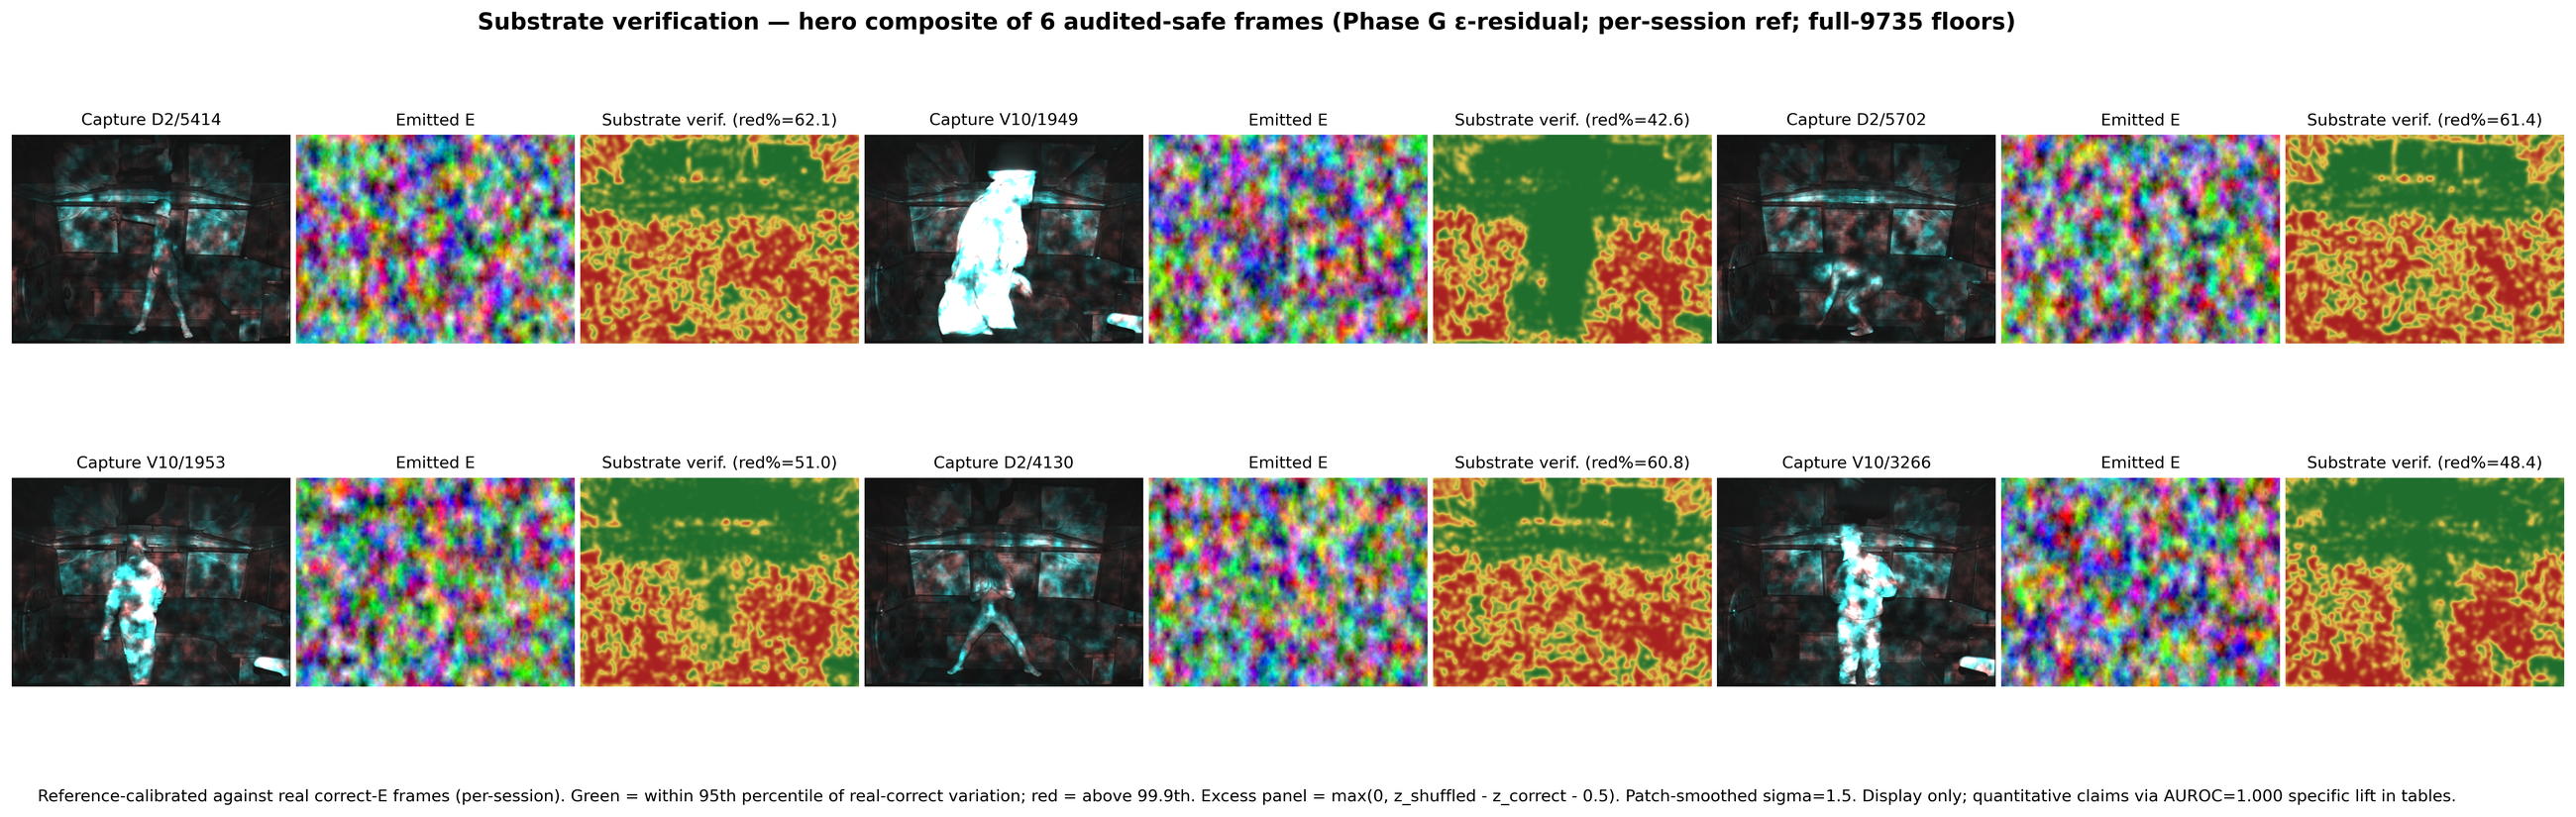
\includegraphics[width=\linewidth]{figures/fig_overview.png}
\caption{System overview and per-frame decision. Six audited-safe high-signal captures (three D2 yoga, three V10), each shown as a triple: the raw camera capture $C$, the emitted chain-coupled pattern $E$ that was projected, and the substrate-verification residual map. The verification map answers one question per frame---is this capture consistent with the recorded chain-coupled emission? Green indicates consistency; red indicates an anomalous (un-coupled) region. Calibrated against real-correct $E$ frames per session; green where the robust $z$ lies below threshold, red above; the excess panel is $z_{\mathrm{two}}$ minus the per-pixel p99.9 floor at margin~0.5; $\sigma=0.0$ (paper detail). Frames are drawn from the \num{9733} body-safe pool ($\text{body\_red} < 0.5\%$); no manual body suppression is applied.}
\label{fig:overview}
\end{figure}

\subsection{What a verifier observes}
\label{sec:system_threat:observable}

The property that makes verification possible is that a genuine recording carries a learnable \emph{physical coupling} between $C_t$ and $E_t$. The projector emits a chain-derived fBm field; the camera records the scene under that field as a raw BayerRG8 frame; and the optical channel imposes a characteristic relationship between the two. This coupling is what the verifier learns to recognize. A useful empirical anchor for what survives the optical channel is an early single-session (D2) characterization: emission RGB structure can be recovered from raw capture at validation PSNR $\approx \SI{26.20}{\decibel}$, whereas direct per-cell XOF byte prediction sits at chance (validation bit accuracy $=0.500$). In other words, the channel acts as an optical low-pass: the coupling that survives to the camera is emission-RGB-style structure, not byte-level XOF detail. This distinction matters for the threat model below, because it bounds which substitutions are optically detectable.

\subsection{Threat model}
\label{sec:system_threat:threat}

The adversary's goal is singular: to have a recording \emph{accepted as authentic} when it is not. Concretely, the adversary wants a verifier to certify a capture as a genuine, chain-coupled photograph of the real scene under the prescribed emission. Two attack avenues realize this goal.

\paragraph{Forge-under-known-$E_{\mathrm{target}}$.} The adversary knows the target emission $E_{\mathrm{target}}$ (it is chain-derived and, in our evaluation, treated as known to the attacker) and synthesizes a fake capture $C_{\mathrm{fake}}$ intended to pass as a genuine capture of the scene under $E_{\mathrm{target}}$. To succeed, $C_{\mathrm{fake}}$ must simultaneously (i)~reproduce the physical coupling that a real capture exhibits with respect to $E_{\mathrm{target}}$ and (ii)~be a realistic raw BayerRG8 capture in its own right. The concrete instantiation of this attacker used throughout this work is the learned editor F-A v1: a \num{42.3}-million-parameter ControlNet-style~\cite{zhang2023controlnet} editor that produces $C_{\mathrm{fake}}$ conditioned on $E_{\mathrm{target}}$ together with source-capture and source-emission hints.

\paragraph{Tamper.} The adversary modifies a genuine recording---substituting, editing, or re-ordering captured frames---while attempting to keep the chain self-consistent. Because the captured bytes are hashed into the next state, any such substitution propagates: a changed $C_t$ implies a changed $S_{t+1}$ and hence a changed expected $E_{t+1}$, so a tampered segment can be exposed by re-walking the chain against a held reference. This is the protocol-level (cryptographic) line of defense and is distinct from the learned verifier; the two are complementary.

\paragraph{Within-attack contrasts used for evaluation.} Beyond a wholesale fake, we evaluate finer substitutions that probe \emph{which} part of the coupling a verifier relies on: pairing a real capture with a temporally mis-aligned or shuffled emission (wrong-$E$), substituting emissions across octaves or channels, and applying fine XOF-level bit-flips to the emission. These are diagnostic perturbations of the emission side of the $(C,E)$ pair rather than full forgeries, and they let us characterize the verifier's sensitivity profile (\Cref{sec:redteam_item1}).

\subsection{Trust assumptions}
\label{sec:system_threat:trust}

The verifier's guarantees are conditioned on the following assumptions.

\begin{itemize}
  \item \textbf{Holder of a chain sample.} Tamper-evidence requires that the verifier (or auditor) holds a trustworthy sample of the chain---at minimum the recorded chain states and capture hashes---against which to check consistency. The closed-loop argument is meaningless to a party that holds neither the chain nor a reference.
  \item \textbf{Honest recording-time hashing and beacon handling.} The protocol assumes the recorder folds the true captured bytes, capture-meta, and a locally verified drand signature into the transition. The chain transition itself does not re-verify the drand signature; a sentinel (round number $0$, value all-zeros) is folded verbatim when the beacon is unavailable, and the verifier notes \texttt{drand\_availability} as \textsc{partial} or \textsc{missing} without gating the pass/fail decision on it.
  \item \textbf{Genuine captures carry learnable coupling.} The learned verifier assumes that real $(C_t, E_t)$ pairs from the operating rig exhibit a consistent physical coupling that fakes and mispairings violate; this is an empirical property of the optical channel established on the two sessions studied here.
  \item \textbf{Known target emission.} The forging adversary is assumed to know $E_{\mathrm{target}}$. This is the strong, conservative assumption: it grants the attacker the very signal the verifier checks against, so success under it is a meaningful test of coupling fidelity rather than of emission secrecy.
\end{itemize}

\subsection{What ``verification'' means here}
\label{sec:system_threat:verification}

Verification in this work is a per-frame consistency test, not an identity, semantic, or content-authenticity judgment. The verifier scores a single $(C_t, E_t)$ pair and asks whether $C_t$ is consistent with the chain-coupled emission $E_t$; it does not attempt to recover the XOF bytes, nor to assert anything about the scene's meaning. The learned instantiation (Phase~G, detailed in \Cref{sec:verifier_method}) is a diffusion-residual scorer: a capture is deemed typical when the noise-prediction residual $\lVert \hat{\epsilon}-\epsilon\rVert^2$ is small for the recorded emission and anomalous when it is large, with the emission entering as a conditioning hint rather than as a denoising target.

Two scope guards bound every claim in this report and are stated here once, to be carried throughout.

\begin{itemize}
  \item \textbf{Same-rig scope.} All results are obtained on a single physical rig across two recording sessions (D2 and V10) of one performer. Generalization claims are \emph{same-rig cross-session} (and, where v9 and v10 are both involved, \emph{same-rig cross-protocol}) only. Nothing here establishes cross-rig, cross-camera, cross-projector, or cross-subject generalization.
  \item \textbf{Attacker scope.} The evaluated forging adversary is F-A v1. A stronger adaptive attacker, F-A v2, exists only as a design specification: it is \emph{not trained} and its trainer code does not exist. Accordingly, this work makes \emph{no} claim of robustness against a strong or adaptive attacker; such robustness is explicitly future work (\Cref{sec:results_redteam}).
\end{itemize}

With the system, the adversary, the trust assumptions, and the meaning of verification fixed, the remainder of the report develops the verifier architecture, its quantitative separability against F-A v1, the localization of the discriminative signal, and the sensitivity of the verifier to graded emission perturbations.

\section{The Truth Beam Protocol \& Cryptographic Chain}
\label{sec:protocol_chain}

The Truth Beam protocol is a tamper-evident video-recording chain. It records a scene not as a passive sequence of frames but as a coupled sequence of \emph{emit--capture--commit} steps, in which each captured frame is cryptographically bound to a deterministic, unpredictable illumination pattern derived from the recording's own history. The construction follows the projector--camera apparatus of the companion patent~\cite{patent2025}, and uses BLAKE3 in its extendable-output (XOF) mode~\cite{blake3} as the deterministic byte source that links the cryptographic and optical layers. This section gives the full method: how a chain state is expanded into a per-channel emission tile, how that tile is rendered and projected, and how the resulting raw capture is folded back into the chain to close a feedback loop that makes any substituted capture detectable. We then describe the two protocol versions exercised in this work (v9 and v10), the binding of an external randomness beacon, the strictly 8-bit data path, and the frame-to-chain offset convention.

\subsection{Overview and notation}
\label{subsec:pc_overview}

We write the chain state at step $t$ as a \SI{32}{byte} value $S_t$, the deterministic emission tile derived at step $t$ as $E_t$, and the raw camera capture at step $t$ as $C_t$. At each step the apparatus (i) derives the emission $E_t$ from the chain state, (ii) projects $E_t$ onto the scene and captures the raw frame $C_t$, and (iii) advances the chain to $S_{t+1}$ by hashing $C_t$ (together with capture metadata and an external beacon) into the next state. Because $C_t$ enters $S_{t+1}$, and $S_{t+1}$ in turn governs the next emission $E_{t+1}$, any attempt to substitute a forged capture for $C_t$ produces a different state and hence a different downstream emission, which a verifier holding a reference sample of the chain can detect. The remainder of the section makes each of these steps precise.

\Cref{fig:overview} shows the per-frame structure that the protocol produces: for each step the raw capture $C$, the projected chain-coupled pattern $E$, and a verification residual answering whether $C$ is consistent with the $E$ that was recorded for that step. The verifier that produces those residuals is described in \Cref{sec:verifier_method}; here we are concerned only with the protocol that generates the $(C_t, E_t, S_t)$ triples.

\subsection{Per-channel BLAKE3-XOF seed derivation}
\label{subsec:pc_seed}

The chain state is the entropy source for the emission, but it is not used directly. Instead the protocol derives three independent per-channel seeds by domain-separated hashing of a chain state $S_{\mathrm{next}}$ (the per-row alignment of this state to a capture is fixed in \Cref{subsec:pc_offset}):
\begin{equation}
\mathrm{seed}_{c} \;=\; \mathrm{BLAKE3}\!\left(\texttt{TB:SEED:}c\texttt{:v8} \,\|\, S_{\mathrm{next}}\right),
\qquad c \in \{R, G, B\},
\label{eq:pc_seed}
\end{equation}
where each $\mathrm{seed}_c$ is \SI{32}{byte} and the domain tags are the literal byte strings \texttt{b"TB:SEED:R:v8"}, \texttt{b"TB:SEED:G:v8"}, and \texttt{b"TB:SEED:B:v8"}. The domain tags carry the version suffix \texttt{v8} even in sessions recorded under the later v9 and v10 chains: the seed and XOF derivation are unchanged across protocol versions, and only the per-row chain-advance transition (\Cref{subsec:pc_chain}) differs between versions. The seed-tag version should therefore not be conflated with the session's chain version.

\subsection{Per-channel 43{,}110-byte expansion into fBm octaves}
\label{subsec:pc_octaves}

Each \SI{32}{byte} seed is expanded by BLAKE3-XOF into exactly \num{43110} bytes per channel. These bytes are partitioned into four fractional-Brownian-motion (fBm) octaves, each a small coarse grid whose byte count equals its pixel count:
\begin{equation}
\underbrace{17\times 30}_{510}
\;+\;\underbrace{34\times 60}_{2040}
\;+\;\underbrace{68\times 120}_{8160}
\;+\;\underbrace{135\times 240}_{32400}
\;=\;\num{43110}\ \text{bytes/channel}.
\label{eq:pc_octaves}
\end{equation}
The implementation derives this total as \texttt{TOTAL\_XOF\_BYTES\_PER\_CHANNEL} $= \sum_{\text{octaves}} h\cdot w$ (\texttt{tile\_params.py}), which evaluates to \num{43110}. The four octaves form a coarse-to-fine pyramid, octave~0 being the lowest-frequency $17\times30$ grid and octave~3 the highest-frequency $135\times240$ grid. The raw XOF output is stored verbatim as unsigned bytes in $[0,255]$; the centering required by the renderer is applied internally rather than persisted, so caches and logs hold the \texttt{raw\_unsigned\_byte} representation and the spec-centered grids are never written to disk.

\subsection{Bit-exact emission-tile rendering}
\label{subsec:pc_render}

The four octave grids are composited into a single full-resolution emission tile of size $\text{TILE\_H}\times\text{TILE\_W} = 1080\times1920$ per channel. The renderer is fully integer and bit-exact, so that the tile a verifier reconstructs from a chain state is byte-identical to the one that was projected. For each octave, the stored bytes are reshaped to $(3, g_h, g_w)$ and centered to signed 16-bit values via $\texttt{byte} - 128$, then upsampled to $(3, 1080, 1920)$ by integer bilinear interpolation with 16-bit fixed-point fractional weights (scale $S = 65536$). The upsampled octaves are accumulated with progressively reduced weight: octave~0 initializes the accumulator at full scale, and each subsequent octave $i$ is added after an arithmetic right shift, $\text{frame} \mathrel{+}= (\text{upsampled} \gg i)$. The final tile is recovered by
\begin{equation}
E \;=\; \mathrm{clamp}\!\left(\left(\text{frame} \gg 16\right) + 128,\; 0,\; 255\right)\ \text{as uint8},
\label{eq:pc_render}
\end{equation}
producing an 8-bit RGB image. The shift-by-$i$ accumulation gives the coarse octaves dominant amplitude and the fine octaves diminishing contribution, which is the fBm spectral profile. The rendered tiles are stored at \texttt{\{session\}/derived/Emissions/tile\_\{t:06d\}.png} as $1080\times1920$ RGB 8-bit PNGs; both sessions are complete, with \num{5992} tiles for D2 and \num{3743} for V10. The renderer used for the verification probes is a documented bit-exact reimplementation of the canonical CUDA/CPU tile generator.

\subsection{Chain-state evolution and tamper-evidence}
\label{subsec:pc_chain}

After $E_t$ is projected and the raw frame $C_t$ is captured, the chain advances by hashing the captured bytes, the capture metadata, and an external beacon into the next state. The capture is bound through its raw hash $\mathit{bayer\_hash}_t = \mathrm{BLAKE3}(C_t)$, a \SI{32}{byte} digest taken over the raw BayerRG8 bytes (the chain log records this as \texttt{bayer\_blake3\_hex}). The capture metadata is a \SI{28}{byte} big-endian struct (format \texttt{>IQQI4s}) comprising the step index $t$ (uint32), the device timestamp and wall-clock time (two uint64 values), the exposure in microseconds (uint32), and a four-byte FourCC pixel-format tag (e.g.\ \texttt{b'RG08'} for BayerRG8).

Under the v9 chain (session D2) the transition is
\begin{equation}
\begin{aligned}
S_{t+1} \;=\; \mathrm{BLAKE3}\big(\,&\texttt{TB:ROW:v9}\,\|\,S_t\\
&\|\,\ell(\mathit{bayer\_hash})\,\|\,\mathit{bayer\_hash}\\
&\|\,\ell(\mathit{meta})\,\|\,\mathit{meta}\\
&\|\,\ell(\mathit{round})\,\|\,\mathit{round}\\
&\|\,\ell(\mathit{rand})\,\|\,\mathit{rand}\,\big),
\end{aligned}
\label{eq:pc_v9}
\end{equation}
where $\ell(\cdot)$ denotes a four-byte big-endian length prefix, $\mathit{meta}$ is the \SI{28}{byte} capture struct, and $(\mathit{round}, \mathit{rand})$ are the drand beacon fields of \Cref{subsec:pc_drand}. Note that under v9 the prior state $S_t$ is concatenated without a length prefix; this differs from v10 below. Because $\mathit{bayer\_hash}_t = \mathrm{BLAKE3}(C_t)$ is folded into $S_{t+1}$, substituting any forged capture $C_t' \neq C_t$ yields a different $\mathit{bayer\_hash}$, hence a different $S_{t+1}$, hence a different seed and a different downstream emission $E_{t+1}$. The feedback loop is therefore closed: tampering with any link propagates an inconsistency into the emission of every subsequent step, detectable by a verifier that holds a reference sample of the chain. We emphasize that the chain transition does not itself re-verify the beacon signature; the recording writer must locally verify drand before passing it in, and the verifier treats missing-beacon sentinels as an availability note rather than a PASS/FAIL gate.

\subsection{Protocol versions: v9 and v10}
\label{subsec:pc_versions}

The two sessions in this work were recorded under different chain versions, and the verifier of \Cref{sec:verifier_method} operates across both, giving a same-rig cross-protocol generalization result (the scope of that claim is discussed in \Cref{sec:results_main_generalization}). Relative to its predecessor, v9 is an attribution-oriented revision whose substantive change is the folding of the drand beacon into the per-row transition; the domain tag bump to \texttt{TB:ROW:v9} reflects that extension.

The v10 chain (session V10) extends v9 with an additional \SI{32}{byte} field, the \emph{ai\_payload\_root}, which commits to AI-agent response frames recorded alongside the capture, and it length-prefixes the prior state $S_t$ in the hash input:
\begin{equation}
\begin{aligned}
S_{t+1} \;=\; \mathrm{BLAKE3}\big(\,&\texttt{TB:ROW:v10}\,\|\,\ell(S_t)\,\|\,S_t\\
&\|\,\ell(\mathit{bayer\_hash})\,\|\,\mathit{bayer\_hash}\\
&\|\,\ell(\mathit{meta})\,\|\,\mathit{meta}\\
&\|\,\ell(\mathit{round})\,\|\,\mathit{round}\\
&\|\,\ell(\mathit{rand})\,\|\,\mathit{rand}\\
&\|\,\ell(\mathit{ai\_root})\,\|\,\mathit{ai\_root}\,\big).
\end{aligned}
\label{eq:pc_v10}
\end{equation}
The distinct domain tag is not cosmetic: it means a v9 chain log cannot be re-walked under v10 (or vice versa), so the two protocols are structurally non-interchangeable.

The ai\_payload\_root is itself a domain-separated commitment. For an empty payload list it takes the sentinel value \texttt{AI\_PAYLOAD\_EMPTY\_ROOT} (32 zero bytes); otherwise it is
\begin{equation}
\mathit{ai\_root} \;=\; \mathrm{BLAKE3}\!\left(\texttt{TB:AI\_PAYLOAD\_ROOT:v10}\,\|\,\ell(32)\,\|\,\mathit{count}\,\|\,{\textstyle\bigl\|}_{k}\,\bigl(\ell(32)\,\|\,p_k\bigr)\right),
\label{eq:pc_airoot}
\end{equation}
where $\mathit{count}$ is a four-byte big-endian count and each $p_k$ is a \SI{32}{byte} BLAKE3 digest of one agent's response text. Payload order is significant. In the V10 session, \num{17} of the \num{3743} rows carry payloads --- six rows with a single payload and eleven with three --- while the remaining \num{3726} rows fold in the empty-root sentinel.

\subsection{drand beacon binding}
\label{subsec:pc_drand}

To bind each step to an external, publicly-verifiable source of unpredictability, the transition folds in the drand quicknet randomness beacon~\cite{drandbeacon}. Two fields are committed: the round number $\mathit{round}$, an 8-byte big-endian \texttt{u64}, and the round value $\mathit{rand}$, the \SI{32}{byte} round randomness (the SHA-256 of the round's BLS signature). The chain log additionally records the observed beacon staleness in milliseconds. As noted above, the writer is responsible for verifying the beacon signature locally before binding it; the transition incorporates the supplied bytes verbatim. When the beacon is unavailable, sentinel values (round number $0$, value all zeros) are folded in and the verifier records a \texttt{PARTIAL}/\texttt{MISSING} availability note without gating the verdict.

\subsection{8-bit end-to-end data path}
\label{subsec:pc_8bit}

The protocol is 8-bit from end to end. BLAKE3-XOF emits raw \texttt{uint8} bytes; the renderer composites and writes 8-bit RGB PNGs; and the camera --- a Sony IMX540 with a native 12-bit ADC --- is configured to deliver 8-bit BayerRG8, so the captured frames have a sensor maximum of $255$. No stage of the emit--capture--commit loop runs above \SI{8}{bit}. (Any earlier ``12-bit packed Bayer'' description was a misnomer arising from the sensor's native ADC depth, not the configured output.) The hardware data path is detailed further in \Cref{sec:hardware}; here the relevant point is that the cryptographic, rendering, and optical layers all operate on the same 8-bit alphabet.

\subsection{Frame-to-chain offset convention}
\label{subsec:pc_offset}

The recording loop fixes the alignment between a capture and the emission committed alongside it, and the implementation is unambiguous. The v9 blocking-mode chain writer --- the only supported capture path, used to record both D2 and V10 --- enforces the invariant that chain-log row $t$ commits the emission that was \emph{live on the projector during} capture $C_t$, namely $E_t = \mathrm{gen}(\mathrm{XOF}(S_t))$. The emission for capture row $t$ is therefore seeded from that same row's chain state $S_t$: $\textit{target\_chain\_row} = \textit{capture\_row} = t$ (offset $0$), and Equations~\eqref{eq:pc_seed}--\eqref{eq:pc_render} are to be read with $S_{\mathrm{next}} = S_t$ for the emission committed at row $t$. Accordingly, in each released chain-log row the \texttt{S\_t\_hex} field, the raw-capture hash \texttt{bayer\_blake3\_hex}, and the \texttt{emission\_live\_*} fields all refer to the same step $t$. We note for completeness that certain auxiliary chain-byte probes and training pipelines elsewhere in this work adopt a shifted alignment ($\textit{target\_chain\_row} = \textit{capture\_row} + 1$, i.e.\ seeding from $S_{t+1}$); that is a verification-side diagnostic choice and \emph{not} the recording convention. The empirically optimal frame-to-chain offset for the optical verifier has not been separately measured on the held-out blocks and remains an open diagnostic, but the recording itself is unambiguous and commits $E_t = \mathrm{gen}(\mathrm{XOF}(S_t))$ per the loop invariant above.

\subsection{Chain-log schema}
\label{subsec:pc_schema}

Each session is accompanied by a single \texttt{chain\_log.csv} recording one row per chain step, preceded by a comment line carrying the session ISO-UTC timestamp and a header row. The D2 (v9) log has 13 columns; the V10 (v10) log has the same 13 columns plus two ai-payload columns, for 15 total. \Cref{tab:pc_chainlog} lists the schema. The D2 log contains \num{5992} records and the V10 log \num{3743}, matching the per-session frame and emission-tile counts.

\begin{table}[t]
\centering
\caption{Chain-log schema. The first 13 columns are common to v9 (D2) and v10 (V10); the final two columns (marked v10) are present only in the v10 log. One comment line (\texttt{\# session\_iso\_utc=...}) and one header row precede the records.}
\label{tab:pc_chainlog}
\small
\begin{tabular}{@{}llp{0.46\linewidth}@{}}
\toprule
Column & Type / size & Description \\
\midrule
\texttt{t} & int & Chain row index; also the capture-file index \\
\texttt{S\_t\_hex} & 32 B (hex) & Chain state $S_t$ \\
\texttt{bayer\_blake3\_hex} & 32 B (hex) & $\mathrm{BLAKE3}(C_t)$ over raw Bayer bytes \\
\texttt{capture\_frame\_id} & int & Aravis/GenICam frame id (metadata only) \\
\texttt{aravis\_device\_timestamp\_ns} & uint64 & Device timestamp (ns) \\
\texttt{capture\_wall\_ns} & uint64 & Host wall-clock at capture (ns) \\
\texttt{emission\_live\_pixel\_blake3\_hex} & 32 B (hex) & Hash of live-queued emission pixels \\
\texttt{emission\_live\_queued\_wall\_ns} & uint64 & Wall-clock when emission was queued (ns) \\
\texttt{meta\_hex} & 28 B (hex) & Capture-meta struct \texttt{>IQQI4s} \\
\texttt{emission\_png\_path} & string & Path to $E_t$ tile PNG \\
\texttt{drand\_round\_number} & uint64 & drand quicknet round number \\
\texttt{drand\_round\_value\_hex} & 32 B (hex) & drand round randomness $\mathit{rand}$ \\
\texttt{drand\_staleness\_ms} & int & Observed beacon staleness (ms) \\
\midrule
\texttt{ai\_payload\_count} & int & (v10) Number of agent payloads at this row \\
\texttt{ai\_payload\_root\_hex} & 32 B (hex) & (v10) ai\_payload\_root commitment \\
\bottomrule
\end{tabular}
\end{table}

Two indexing details matter for downstream use. First, the capture-file index equals the chain row index $t$, \emph{not} the Aravis \texttt{capture\_frame\_id}; row~0 carries \texttt{capture\_frame\_id} $= 4$, and the id advances in strides of four as a GenICam hardware-tick artifact. The chain commits at approximately \SI{2.5}{\hertz}, one physical exposure per chain step; the stride-of-four id should not be read as a \SI{10}{\hertz} frame rate. Second, the \texttt{bayer\_blake3\_hex} field is the digest of the raw capture and is the value folded into $S_{t+1}$, distinct from \texttt{emission\_live\_pixel\_blake3\_hex}, which records the emission pixels and is not part of the chain transition. Together with the bit-exact renderer of \Cref{subsec:pc_render}, this schema makes the entire $(S_t, E_t, C_t)$ trajectory reconstructible and auditable from the logged state alone.

\section{Capture and Emission Pipeline}
\label{sec:hardware}

This section documents the physical capture and emission pipeline that produces every $(E_t, C_t)$ pair consumed downstream by the verifier, together with the on-disk representation, sampling rate, normalization, and dataset inventory. A guiding principle throughout is that the entire Truth Beam loop is \SI{8}{bit} end-to-end: the BLAKE3-XOF byte stream, the rendered emission tiles, and the camera capture all live in $[0,255]$, and no stage of the loop operates at higher bit depth. The protocol-level chain semantics that bind $E_t$ and $C_t$ are treated in \Cref{sec:protocol_chain}; here we describe the optics, sensor configuration, and data handling that those semantics ride on.

\subsection{Sensor and bit depth}
\label{sec:hardware:sensor}

The capture camera is built around a Sony IMX540 image sensor. The sensor possesses a \SI{12}{bit} analog-to-digital converter natively, but the camera is deliberately configured to deliver \SI{8}{bit} BayerRG8 frames rather than its full ADC depth. As a consequence the sensor maximum value seen by every downstream stage is $255$, and the protocol is \SI{8}{bit} from emission synthesis through capture. We emphasize this configuration explicitly because an earlier internal description characterized the format as a ``12-bit packed Bayer'' final specification; that phrasing was a misnomer. The \SI{12}{bit} figure refers only to the sensor's native ADC capability, not to the bit depth at which any TB artifact is rendered, projected, captured, hashed, or stored. The BLAKE3-XOF stage \cite{blake3} expands to raw \texttt{uint8} bytes, the renderer writes \SI{8}{bit} RGB PNGs, and the camera returns BayerRG8: there is no point in the loop above \SI{8}{bit}.

\subsection{Raw frame format and color filter array}
\label{sec:hardware:raw}

Each raw capture frame $C_t$ is written to disk as a headerless block of exactly \num{24472000} bytes of \texttt{uint8} data, with no embedded metadata or padding. The frame is row-major with shape $(H, W) = (4600, 5320)$, and the byte count is exact: $4600 \times 5320 = \num{24472000}$. The color filter array is RGGB, i.e.\ within each $2\times2$ Bayer quad the top-left pixel is red, the top-right and bottom-left are the two green channels ($G_1$, $G_2$), and the bottom-right is blue. This pattern was verified against on-disk nearest-neighbor previews by byte-equality on a representative row.

A subtlety worth recording for any reimplementation is the demosaicing flag. Although the camera SDK reports the CFA as BayerRG8, the correct OpenCV demosaic constant for this physical layout is \texttt{cv2.COLOR\_BayerBG2RGB\_EA}, \emph{not} \texttt{cv2.COLOR\_BayerRG2RGB}. The naming discrepancy reflects a red/blue convention difference between the camera vendor's labeling and OpenCV's internal naming; applying the literal \texttt{BayerRG2RGB} flag would wrongly swap the red and blue channels. Validation against the nearest-neighbor previews under the \texttt{BayerBG2RGB\_EA} flag yielded per-channel Pearson correlations of $1.0$ (R), $0.996$ (G), and $0.991$ (B), confirming the flag choice.

\subsection{Emission tiles and projection}
\label{sec:hardware:emission}

The emission target $E_t$ projected at chain step $t$ is rendered at $1080 \times 1920$ ($H \times W$); equivalently, the PIL image size is $W{=}1920$, $H{=}1080$. Each tile is an \SI{8}{bit}-per-channel RGB PNG stored as \texttt{uint8} in $[0,255]$ at the path \texttt{\{session\}/derived/Emissions/tile\_\{t:06d\}.png}; the dataset loader divides by $255$ to obtain a \texttt{float32} image in $[0,1]$ before any further normalization. These tiles are the images that were actually projected during recording, generated deterministically from the chain state via the bit-exact octave renderer detailed in \Cref{sec:protocol_chain}. The projector emits at $1920 \times 1080$. The patent \cite{patent2025} gives, as exemplary values, a projector refresh of approximately \SI{16}{\milli\second} and a configuration of $1920\times1080$ projected against $5360\times4600$ detected; these are exemplary figures from the patent rather than measured quantities in this dataset, and we note that the patent's exemplary detected width ($5360$) differs from the actual on-disk raw frame width ($5320$) and should not be conflated with it. The $1080\times1920$ ($H\times W$) schema notation and the $1920\times1080$ projector-emit notation describe the same $2.07$\,MP frame in transposed axis order.

\subsection{Commit rate and the \texttt{capture\_frame\_id} stride artifact}
\label{sec:hardware:rate}

The chain commits at approximately \SI{2.5}{\hertz}, and the correct physical reading of this rate is \emph{one physical exposure per chain step}: each chain advance corresponds to a single captured frame projected under a single emission tile. This point requires care because the GenICam metadata field \texttt{capture\_frame\_id} advances in strides of four (for example, chain row $0$ carries \texttt{capture\_frame\_id}${=}4$). That stride is a GenICam hardware-tick artifact of the acquisition layer; it is \emph{not} evidence of a \SI{10}{\hertz} acquisition with a one-in-four commit policy, and the camera should not be described as running at \SI{10}{\hertz}. The authoritative frame index is the chain row index $t$: on-disk capture files are named \texttt{frame\_\{t:06d\}.raw} where $t$ is the chain row, and \texttt{capture\_frame\_id} is retained as metadata only. We adopt the convention throughout that ``frame $t$'' means chain row $t$, with one physical exposure per row.

\subsection{Normalization and black-level handling}
\label{sec:hardware:norm}

Training-time normalization is applied at dataset-load time as a per-channel robust standardization: each channel is centered on its median and scaled by $\mathrm{IQR}/1.349$, where the interquartile range divided by $1.349$ is the robust analogue of the standard deviation under a Gaussian assumption. Crucially, both statistics are computed on training rows only, so that held-out evaluation frames do not leak into the normalization parameters. This method was adopted under an audit mandate, replacing an earlier naive division by $255$.

No black-level (dark-pedestal) subtraction is applied. The capture manifest records \texttt{black\_level}${=}0$ with \texttt{black\_level\_source}${=}$``\texttt{no\_measurement\_found}''. This value of zero should not be read as a measured dark level: it records the \emph{absence} of any measured dark-frame or pedestal value anywhere in the calibration, hardware-setup, or scripts trees. Black-level subtraction is therefore explicitly forbidden until a measured value is confirmed, precisely so that an unverified pedestal estimate cannot silently bias the residual statistics on which verification depends.

\subsection{Dataset inventory}
\label{sec:hardware:dataset}

The dataset comprises two recording sessions captured on the same rig with a single human performer: D2 (\texttt{cittadel\_first\_human}) with \num{5992} chain rows, and V10 (\texttt{cittadel\_v10\_mainnet\_improv}) with \num{3743} chain rows. Both sessions are complete in the sense that every chain row $t$ has a corresponding emission tile \texttt{tile\_\{t:06d\}.png} and raw capture \texttt{frame\_\{t:06d\}.raw}, giving \num{9735} frames in total across the two sessions. The two sessions differ in their chain protocol version (D2 under the v9 chain, V10 under the v10 chain), a difference treated in \Cref{sec:protocol_chain}; for the present purposes they are two physically homogeneous same-rig captures. The performer is the same individual in both sessions but is dressed differently in each (different costume and mask --- yoga attire in D2, an improv costume in V10), so the sessions are not visually identical at the subject level. \Cref{tab:hw_inventory} summarizes the per-session counts and the per-frame storage footprint.

\begin{table}[t]
\centering
\caption{Per-session capture inventory. Raw frame size is exact ($4600\times5320\times\SI{1}{byte}$); raw totals are decimal gigabytes ($10^9$\,B). Both sessions are complete: one raw capture and one emission tile per chain row.}
\label{tab:hw_inventory}
\begin{tabular}{lrrr}
\toprule
Session & Chain rows / frames & Raw Bayer total & Emission tiles \\
\midrule
D2 (\texttt{cittadel\_first\_human})        & \num{5992} & \SI{146.64}{\giga\byte} & \num{5992} \\
V10 (\texttt{cittadel\_v10\_mainnet\_improv}) & \num{3743} & \SI{91.60}{\giga\byte}  & \num{3743} \\
\midrule
Total & \num{9735} & \SI{238.23}{\giga\byte} & \num{9735} \\
\bottomrule
\end{tabular}
\end{table}

Each raw frame is \num{24472000} bytes, so the per-session raw Bayer footprints are $\num{5992}\times\num{24472000} = \SI{146.64}{\giga\byte}$ for D2 and $\num{3743}\times\num{24472000} = \SI{91.60}{\giga\byte}$ for V10, totaling \SI{238.23}{\giga\byte} of raw capture. The emission tile set occupies \SI{23.82}{\giga\byte} across the \num{9735} PNGs, and the per-session chain logs are negligible (a few megabytes each). All raw frames are treated as read-only and are never modified in place.

\paragraph{Scope and privacy.} Both sessions feature an identifiable human performer, so any public release of raw frames, emission tiles, derived previews, or RGB thumbnails is a privacy and consent matter, and the standing display rules forbid any manual suppression of body or person regions in promoted artifacts. We also flag the scope of the dataset explicitly: this is a same-rig, single-operator, two-session corpus. It is suitable for same-rig cross-session and cross-protocol analysis, but it does not on its own support any cross-rig, cross-camera, cross-projector, or cross-subject claim. Two open calibration items are surfaced here for completeness and carried into any release manifest: the measured black level is unknown (recorded as $0$ with source ``\texttt{no\_measurement\_found}'', no subtraction applied), and the projector-pipeline lock status is unconfirmed while the camera photometry is locked.

The end-to-end pipeline---each raw $C_t$ paired with the emission $E_t$ projected at the same chain step and the resulting per-pixel verification residual---is illustrated for representative captures in \Cref{fig:overview} of \Cref{sec:system_threat}; the quantitative separability claims that such illustrations visualize are reported in \Cref{sec:results_main}.

\section{Verification Methodology}
\label{sec:verifier_method}

The verifier of record for the Truth Beam substrate is \emph{Phase~G}: a custom epsilon-prediction U-Net trained as a conditional density model over genuine $(C_t, E_t)$ capture--emission pairs and used as an anomaly scorer rather than a generator. We emphasise at the outset that Phase~G never denoises an image and never synthesises a capture. It is a diffusion model only in the sense that it learns to predict the noise that was added to a known-genuine capture under a forward process conditioned on the emission that was projected at that step; the magnitude of its noise-prediction residual $\lVert \hat{\epsilon}-\epsilon \rVert^2$ then serves as the verification score. This section details the network, its conditioning pathway, the training objective and corpus, the residual-energy scoring rule, and the architecture- and data-matched shuffled control that establishes the result is driven by genuine chain-coupling and not by generic emission statistics or an architectural artifact. The scope of every claim is the same-rig, two-session corpus (D2 and V10); we make no cross-rig, cross-camera, cross-projector, or cross-subject claim anywhere in this section.

\subsection{Network architecture}

The backbone is a custom epsilon-prediction U-Net, denoted \texttt{DiffusionDiagnosticUNet}, with \num{39770000} trained parameters (39.77M) at the canonical checkpoint (step \num{25000}). It is deliberately \emph{not} a diffusion transformer (DiT) and \emph{not} a Stable Diffusion model; it is a compact, purpose-built U-Net tailored to the packed colour-filter-array (CFA) representation of the raw capture. The network operates on a four-channel packed CFA input ($\text{in\_ch}=4$) and predicts a four-channel noise field $\hat{\epsilon}$ of matching shape ($\text{out}=4$).

The encoder/decoder has four down-sampling and four up-sampling scales built from residual blocks. The base channel width is $\text{base\_ch}=96$, and the channel multipliers $(1,2,4,4)$ give per-stage channel counts of $(96,192,384,384)$; the two deepest stages share a width of 384 channels. Self-attention is applied at the deepest scale only ($\text{attn\_at}=(\mathrm{False},\mathrm{False},\mathrm{False},\mathrm{True})$), which restricts the (quadratic) attention cost to the most coarsely sampled feature map while leaving the shallower, higher-resolution stages purely convolutional --- a standard cost--capacity trade-off for image-scale U-Nets.

Phase~G is evaluated full-frame at an operating resolution of $768\times1024$. The packed-CFA capture is cropped (region $y\in[0,1704]$, $x\in[155,2433]$ from the $(4,2300,2660)$ packed tensor) and resampled with area interpolation; the emission is resized from its native $(3,1080,1920)$ tile to the same grid. No tiling, patching, or temporal context is used: each $(C_t,E_t)$ pair is scored independently, frame by frame. We note the modest aspect-ratio adjustment this entails (cropped aspect $\approx 0.748$ resampled to $0.75$, a distortion of $\approx 0.3\%$); the shuffled control below shares this exact preprocessing, so any such artifact is differenced out of the headline comparison.

\subsection{ControlNet-style emission conditioning}

A central design decision is \emph{how} the emission $E_t$ enters the network. We do not concatenate $E_t$ to the camera input $C_t$. Instead, $E_t$ is conditioned in via a ControlNet-style hint pathway~\cite{zhang2023controlnet}. A dedicated \emph{HintEncoder} --- a four-stage strided $3\times3$ convolutional stack (stride 2 at each stage, $/16$ total down-sampling) with GroupNorm and GELU nonlinearities --- produces a multi-scale embedding of the emission hint. At each U-Net scale the encoded hint is injected by \emph{addition} into the down-path features through a per-scale zero-convolution adapter:
\[
\text{fused}_\ell \;=\; \text{down}_\ell(\text{prev}) \;+\; \text{adapter}_\ell\!\big(\text{HintEncoder}_\ell(E)\big),
\]
with one $1\times1$ zero-initialised convolution per scale (four adapters in total). Because the adapters are zero-initialised, the network's output at the start of training is exactly the unconditional model: the emission hint contributes nothing until training ramps it up, so any learned dependence on $E$ is acquired, not assumed. The hint input carries $\text{hint\_in\_ch}=11$ channels, a layout inherited from the F-A~v1 editor's hint encoder; the exact per-channel composition is an inherited implementation detail rather than a quantity we re-derive here.

To keep the conditional pathway honest, training applies classifier-free-guidance-style conditioning dropout: with probability $\text{cond\_drop\_prob}=0.2$, the emission hint is zeroed for a training example. This both regularises the conditioning and makes available, at evaluation time, a meaningful \emph{unconditional} reference (the same network with $E$ zeroed), against which the value of the genuine emission can be measured.

\subsection{Diffusion objective and forward process}

Conditioning aside, the training objective is standard epsilon-prediction. We adopt the denoising diffusion probabilistic model framework~\cite{ho2020ddpm} with the cosine noise schedule of Nichol \& Dhariwal~\cite{nicholdhariwal2021} (offset $s=0.008$) over $T=1000$ diffusion timesteps. The diffusion timestep $\tau$ is sampled uniformly from $\{1,\dots,1000\}$. To avoid clashing with the chain index $t$ of $C_t, E_t, S_t$, we write $x_0$ for the clean diffusion target (a genuine capture, $x_0 \equiv C_t$) and $x_\tau$ for its noised version. The forward (noising) process is the usual closed-form $q$-sample,
\[
x_\tau \;=\; \sqrt{\bar{\alpha}_\tau}\,x_0 \;+\; \sqrt{1-\bar{\alpha}_\tau}\;\epsilon,
\qquad \epsilon \sim \mathcal{N}(0,\mathbf{I}),
\]
with $\bar{\alpha}_\tau$ the cumulative product of the cosine schedule. The model is trained to predict the injected noise from the noised capture and the emission hint, under the simple mean-squared objective
\[
\mathcal{L} \;=\; \mathbb{E}_{\tau,\epsilon}\,\big\lVert \hat{\epsilon}(x_\tau, E, \tau) - \epsilon \big\rVert^2,
\]
with conditioning dropout applied as above. There is no perceptual term, no adversarial term, and no auxiliary classifier: the network learns only to model the noise residual of a genuine capture given its genuine emission.

\subsection{Training corpus and optimisation}

Phase~G is trained on real, same-rig capture--emission pairs drawn from two recording sessions: D2 (\num{5992} frames, recorded under the v9 chain) and V10 (\num{3743} frames, recorded under the v10 chain). Training therefore spans two chain protocols on the same rig, which underlies the same-rig cross-protocol observation discussed in \Cref{sec:results_main}; it is not a cross-rig statement. Held-out evaluation blocks are excised from training with a guard band: \num{1200} D2 frames and \num{500} V10 frames (\num{1700} total) are held out, a guard band of \num{60} frames brackets each held-out block, and the remaining training rows are stride-decimated (stride 3, $\approx\num{2478}$ training rows). The D2 held-out blocks are $(1298,1698)$, $(2796,3196)$, $(4294,4694)$ and the V10 blocks are $(1110,1360)$, $(2345,2595)$.

Optimisation runs for \num{25000} steps with AdamW~\cite{loshchilov2019adamw} at learning rate $10^{-4}$ on a cosine learning-rate schedule with a \num{500}-step linear warm-up, with batch size 2 per GPU across 8 GPUs (effective batch 16) under bf16 autocast. Training wall time is approximately \SI{17000}{\second} ($\approx 4.7$ hours) on $8\times$ A100. The epsilon-prediction MSE converges to $\approx 5\times10^{-4}$ (step-\num{25000} batch loss \num{0.000626}; per-batch loss is noisy at batch size 2). No validation-loss curve was logged during training, so model selection is on the final checkpoint; we note this as a limitation in the absence of an early-stopping diagnostic.

\subsection{Residual-energy scoring}

At inference Phase~G does not run the reverse diffusion process. The verification score for a candidate pair $(C,E)$ is the energy of the noise-prediction residual,
\[
\text{score}(C,E) \;=\; \big\lVert \hat{\epsilon} - \epsilon \big\rVert^2 ,
\]
evaluated under the model's own forward process. To make the score stable and timestep-aware we fix five evaluation timesteps spanning the schedule, $\mathrm{ALL\_TIMESTEPS}=(50,150,300,500,750)$, and average over $K_{\mathrm{NOISE}}=4$ independent noise draws per $(C,E,\tau)$. Each noise draw is seeded by the global frame index so the score is reproducible across evaluation shards. The total cost per scored pair is therefore $5\times4 = 20$ forward passes, with the per-pair MSE averaged over those passes. Benchmarked on an A100 in bf16, a single forward pass takes \SI{329}{\milli\second} (batch 1, $\tau=300$, mean of 20 reps), so a full $(C,E)$ score is $\approx\SI{6.6}{\second}$ at batch 1, or $\approx\SI{1.75}{\second}$ with the $K=4$ noise samples batched.

The interpretation is direct: a genuine pair, whose capture lies in the high-density region of the conditional model given its true emission, yields a small residual; a mispaired or substrate-altered pair yields a larger residual. Empirically the discriminative signal is strongest at small $\tau$ and decays as $\tau$ rises, consistent with the substrate signature residing in fine, low-noise structure: on the D2 held-out blocks the per-timestep wrong-versus-correct gap falls from $\Delta_{\text{wrong}}\approx\num{0.00594}$ at $\tau=150$ to $\approx\num{0.00339}$ at $\tau=300$ and $\approx\num{0.00165}$ at $\tau=500$, while per-timestep separability remains saturated (AUROC~$=1.000$) at every reported timestep. \Cref{fig:zhist,fig:ecdf} present the distributional form of this score across the corpus, and \Cref{fig:atypicality} shows its spatial footprint.

\begin{figure}[t]\centering
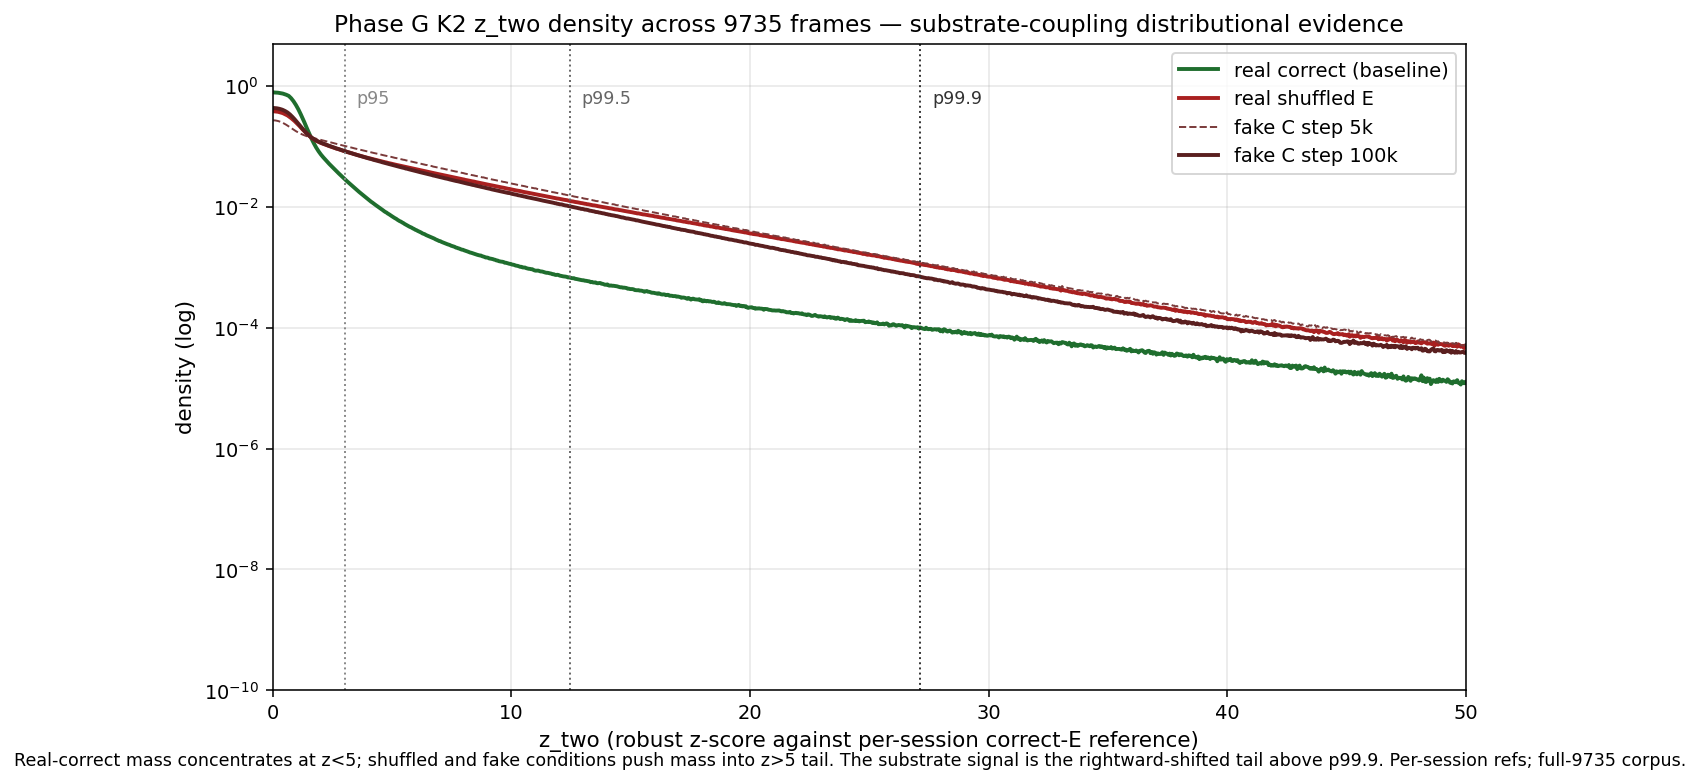
\includegraphics[width=\linewidth]{figures/fig_zhist.png}
\caption{Distributional evidence for chain-coupling. Per-pixel $z_{\text{two}}$ log-density across \num{9735} frames for four conditions: real-correct (baseline), real-shuffled $E$, synthetic $C$ at training step 5k, and step 100k. Real-correct mass concentrates at $z<5$; shuffled and synthetic conditions carry heavy right tails. The discriminative substrate signal is the rightward-shifted tail above the p99.9 percentile. $z_{\text{two}}$ is a robust $z$-score against the per-session correct-$E$ reference; percentile markers (p95, p99.5, p99.9) are drawn from the full-\num{9735} corpus.}
\label{fig:zhist}
\end{figure}

\begin{figure}[t]\centering
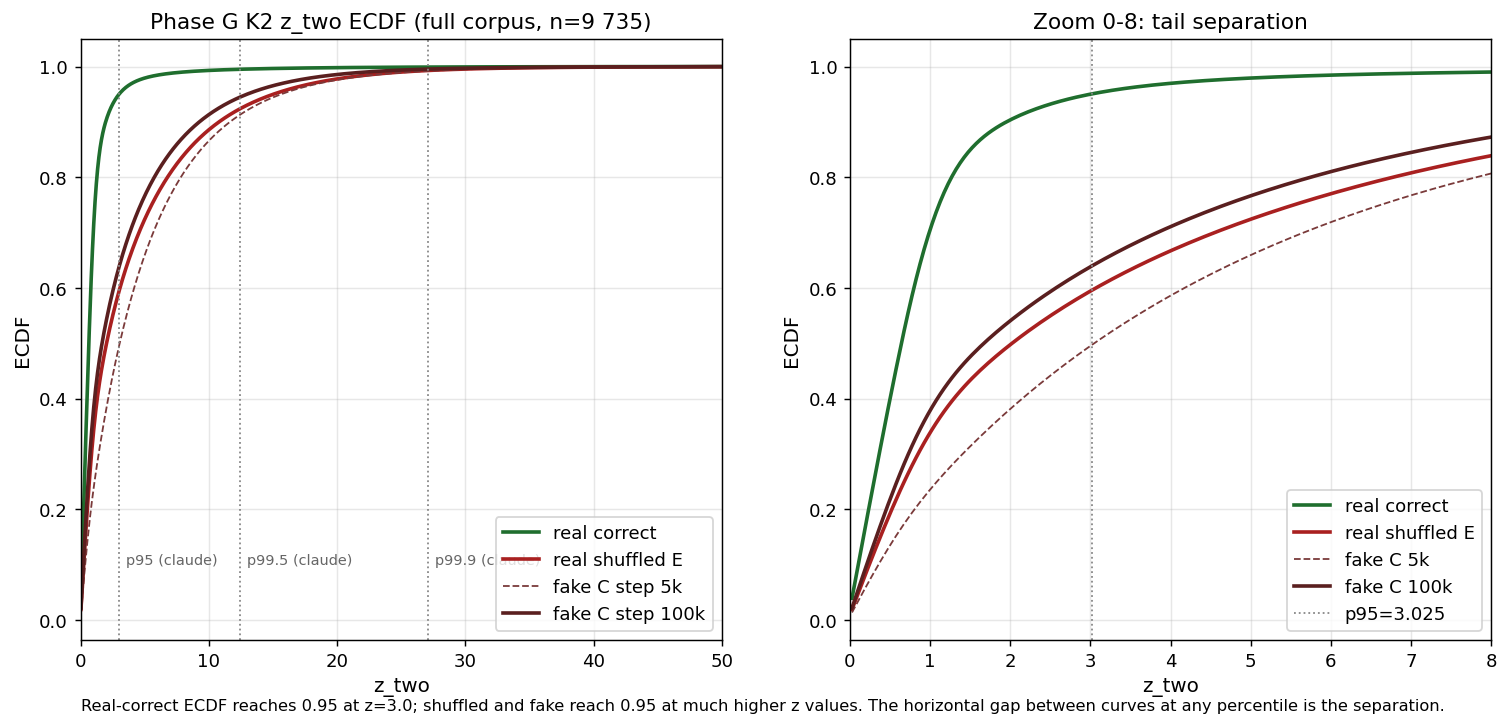
\includegraphics[width=\linewidth]{figures/fig_ecdf.png}
\caption{Empirical CDF of $z_{\text{two}}$ (full corpus, $n=\num{9735}$). Left: full range; right: zoom to $z\in[0,8]$ showing tail separation. The real-correct ECDF reaches $0.95$ at $z=3.0$, while shuffled and synthetic conditions reach $0.95$ only at substantially higher $z$. The horizontal gap between curves at any percentile is the per-pixel separation margin. Per-session reference; percentile markers from the full-\num{9735} corpus.}
\label{fig:ecdf}
\end{figure}

\subsection{The shuffled-E control}

A near-perfect verifier raises an immediate question: is the network truly detecting the physical coupling between a capture and \emph{its own} emission, or is it merely exploiting generic statistics of the emission images, or an artifact of the architecture and training recipe? To answer this we train a second model that is \emph{identical in every respect} --- same \texttt{DiffusionDiagnosticUNet} architecture, same \num{39770000} parameters, same hint pathway and zero-conv adapters, same cosine schedule, same $T=1000$, same corpus, same optimiser, same step budget, same held-out blocks, and the identical $768\times1024$ preprocessing --- with exactly one difference: the genuine pairing between capture and emission is destroyed by \emph{shuffling}. The shuffled model is trained to predict the noise of capture $C_t$ conditioned on a mismatched emission. If the main model's discrimination came from generic emission statistics or from the network/recipe rather than from genuine chain-coupling, the shuffled model would inherit it; if it came from the physical coupling, the shuffled model has nothing to learn and must sit at chance.

The shuffled control sits at chance. Its correct-versus-wrong separability is $\mathrm{AUROC}\approx 0.5006$ (D2 $0.5006377$, V10 $0.500625$), and its mean residual gap between correct and wrong emissions is $\Delta_{\text{wrong}}\approx 10^{-7}$ (D2 $6.98\times10^{-8}$ with 95\% CI $[3.89,\,11.8]\times10^{-8}$; V10 $1.39\times10^{-7}$). By contrast the main model achieves $\mathrm{AUROC}=1.000$ with $\Delta_{\text{wrong}}\approx 4\times10^{-3}$ --- roughly five orders of magnitude larger. The shuffled control's $\Delta_{\text{wrong}}$ confidence interval technically excludes zero, but the effect is so many orders of magnitude smaller than the main model's that it is operationally indistinguishable from chance. This control is the load-bearing falsification test: because it differs from the main model only in the real-versus-shuffled pairing, it isolates the contribution of genuine chain-coupling and rules out generic emission statistics and an architecture/recipe artifact as the source of the separation. It does not by itself exclude every conceivable shortcut --- confounds that survive identical preprocessing, such as session-level idiosyncrasies, are addressed separately by the cross-session ablation of \Cref{sec:results_main_generalization}.

It is important to keep the shuffled control distinct from the offset-based ``wrong-$E$'' used in the headline AUROC. The headline correct-versus-wrong AUROC pairs a genuine capture against \emph{temporally mispaired real emissions} (frame offsets $\{-2,+2,-15,+15,+30\}$ and the lag sweep); the shuffled control instead retrains the entire model under a destroyed pairing. The two are complementary: the offset evaluation shows the main model resolves the correct emission against close temporal neighbours, while the shuffled control shows the capability itself is not an artifact. A separate synthetic-positive control (an isotropic photometric injection, $\mathrm{blur}(E)$ added to $C$) confirms the scoring pipeline can detect an $E$-dependent signal it is meant to detect ($\mathrm{AUROC}=1.000$, $\Delta_{\text{wrong}}\approx 1.1$--$1.2\times10^{-3}$); we caution, per its own design, that an isotropic photometric injection may have different spectral structure from a real chain signal, so it corroborates the pipeline rather than the main result.

\subsection{Unconditional reference and multi-method cross-checks}

The conditioning-dropout design also yields an \emph{unconditional} reference (the trained main model evaluated with $E$ zeroed). Comparing a genuine pair against this reference measures how much the true emission lowers the residual relative to having no emission at all; the resulting correct-versus-unconditional AUROC is $0.977$ (D2) and $0.942$ (V10). This is necessarily a softer contrast than correct-versus-wrong, because the zeroed-$E$ input is itself somewhat out of distribution; we report it as supporting evidence for emission-dependence, not as the headline.

Finally, we cross-check the Phase~G verdict against additional methods on genuine captures (\Cref{fig:multimethod}). Phase~G and a binder-residual method are treated as verifier-tier; autoencoder taps (AE-64f, AE-DGW) are shown for cross-checking only and are explicitly labelled \textsc{diagnostic}, because they exhibit weak coupling-specificity and are not relied upon as verifiers. On genuine frames all four methods agree on a typical (low-residual) verdict, but only the verifier-tier methods carry quantitative weight in this report.

\begin{figure}[t]\centering
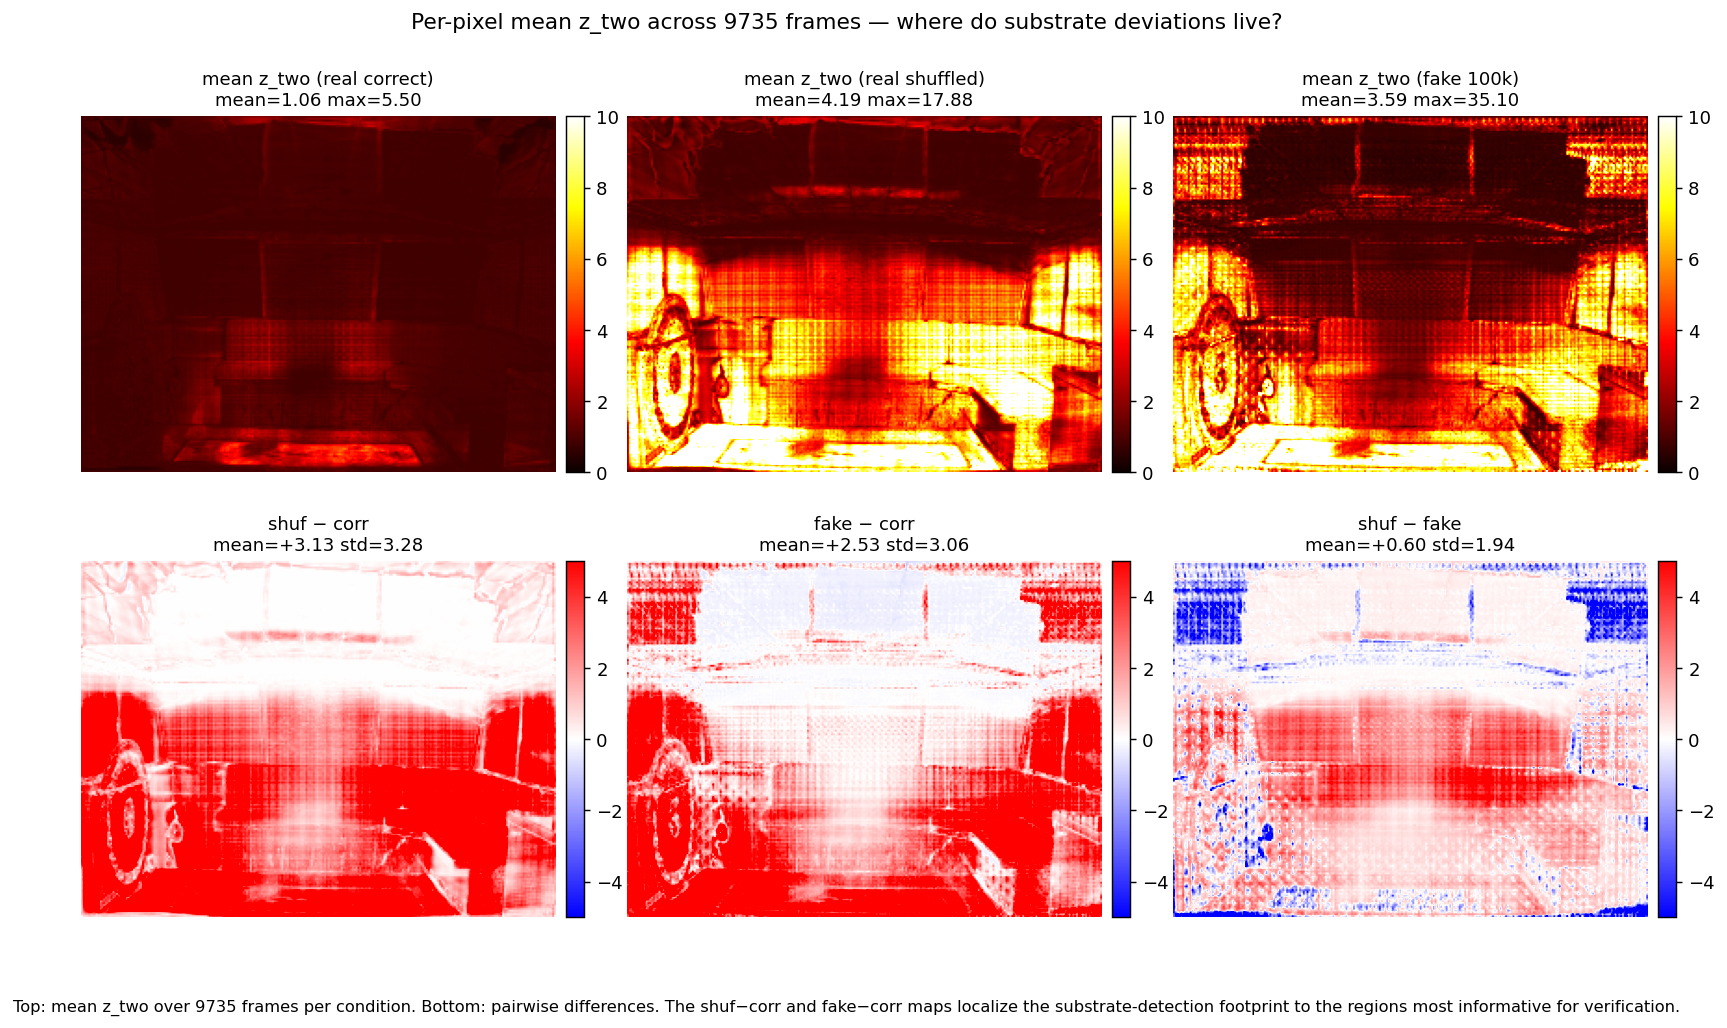
\includegraphics[width=\linewidth]{figures/fig_atypicality.png}
\caption{Spatial footprint of the substrate signature. Top: per-pixel mean $z_{\text{two}}$ across \num{9735} frames for real-correct (mean $1.06$), real-shuffled ($4.19$), and synthetic-100k ($3.59$) conditions. Bottom: pairwise differences (shuffled $-$ correct, synthetic $-$ correct, shuffled $-$ synthetic). The shuffled-minus-correct and synthetic-minus-correct maps localise the substrate-detection footprint to the frame regions most informative for verification, concentrated away from the central subject. Computed over the full \num{9735}-frame corpus with per-session references; no per-frame normalization.}
\label{fig:atypicality}
\end{figure}

\begin{figure}[t]\centering
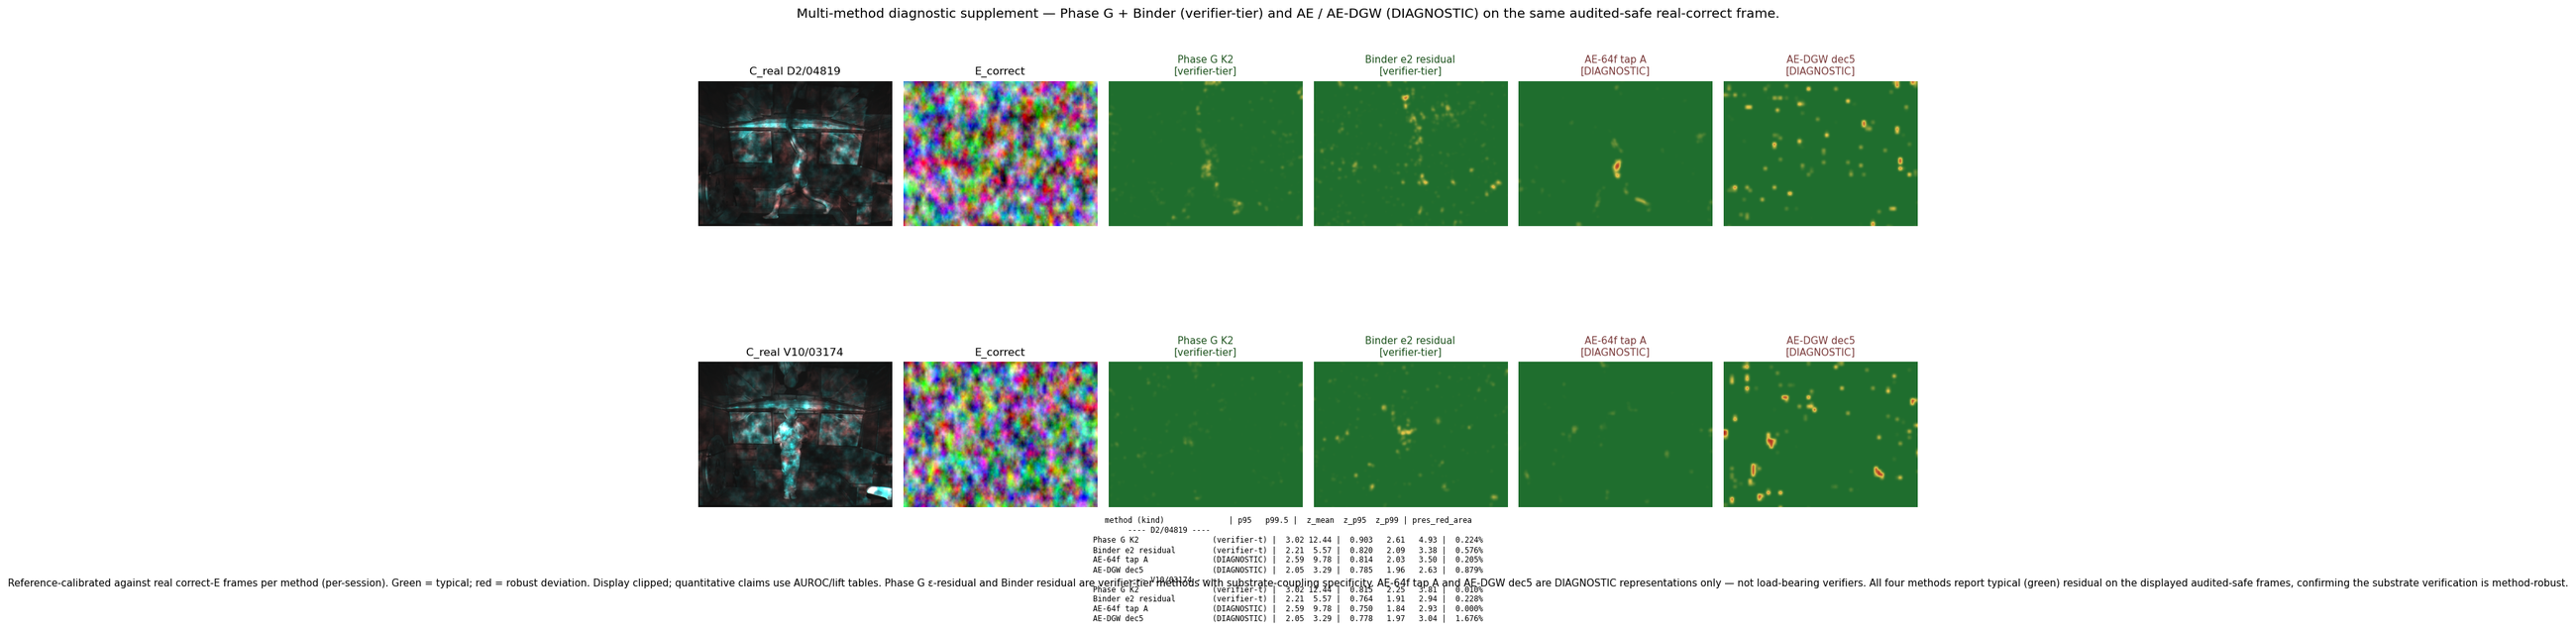
\includegraphics[width=\linewidth]{figures/fig_multimethod.png}
\caption{Multi-method agreement on genuine captures. Two audited-safe real-correct frames (D2 row 4819, V10 row 3174) scored by four methods: Phase~G K2 and Binder e2 (verifier-tier) and AE-64f tap A and AE-DGW dec5 (labelled \textsc{diagnostic}, not verifier-tier). All four report typical (green) residual on these genuine frames. Each method uses its own per-session reference with common thresholds within the panel; display is clipped; quantitative claims rest on the results reported in the text, not on this display. The AE methods are shown for cross-checking only and are not used as verifiers because they exhibit weak coupling-specificity.}
\label{fig:multimethod}
\end{figure}

\subsection{Scope and limitations of the methodology}

Two methodological scope guards apply throughout. First, the held-out evaluation blocks are drawn from the same two sessions used for training, so the $\mathrm{AUROC}=1.000$ result measures \emph{within-session} (same-rig) generalisation; cross-session generalisation is established separately by the single-session ablations of \Cref{sec:results_main_generalization}, and nothing in this work establishes cross-rig, cross-camera, cross-projector, or cross-subject generalisation. Second, the scoring rule is deliberately a residual-\emph{energy} statistic ($\epsilon$-MSE), which (as developed in later sections) is dominated by high-frequency structure; alternative scoring functions reweight which regions of the residual field carry the signal, and the choice of $\epsilon$-MSE is a design decision rather than a unique optimum. The methodology described here is what the remaining results sections evaluate; robustness against a trained, adaptive forger (the stronger F-A~v2 attacker, which is in design only and not trained) is out of scope for this methodology and is treated strictly as future work.

\section{Results I: Learnable Chain-Coupling, Verifier Accuracy and Generalization}
\label{sec:results_main}

This section reports the central empirical claim of the system: that a genuine
Truth Beam recording contains a learnable physical coupling between the captured
raw frame $C_t$ and the chain-derived emission $E_t$, and that this coupling is
strong enough to support a near-perfect verifier on held-out data. We present
the headline verifier accuracy, the control experiment that isolates the
coupling signal from generic emission statistics and architecture artifacts, the
frame-level operating-point analysis on the full corpus, and the same-rig
cross-session and cross-protocol generalization result. We are deliberate about
scope: every quantitative claim below is a \emph{same-rig} result over two
recording sessions (D2 and V10) of a single performer, and the only trained
adversary exercised is F-A~v1. We make no cross-rig,
cross-camera, cross-projector, or cross-subject claim, and no claim of
robustness against a stronger adaptive attacker; those limits are restated
explicitly at the points where they bind. Throughout, held-out evaluation
scores a fixed subsample of the held-out blocks: $n=198$ frames for D2
(66 from each of its three blocks) and $n=200$ for V10 (100 from each of
its two blocks).

\subsection{Headline verifier accuracy}
\label{sec:results_main_headline}

The load-bearing verifier is the Phase~G diffusion model (\Cref{sec:verifier_method}):
a custom \num{39.77}M-parameter $\epsilon$-prediction U-Net with ControlNet-style
emission conditioning, operating frame-by-frame on a single $(C_t, E_t)$ pair.
It never denoises; it scores a capture by the noise-prediction residual
$\lVert \hat{\epsilon}-\epsilon\rVert^2$, averaged over five fixed evaluation
timesteps $\{50,150,300,500,750\}$ and $K_{\text{NOISE}}=4$ noise samples per
$(C,E,t)$. A capture that is consistent with its recorded chain-coupled emission
yields a low residual; a capture paired with the wrong, shuffled, or synthetic
emission yields a higher residual.

On held-out evaluation blocks the verifier separates the correct emission $E_t$
from temporally mispaired (offset) wrong emissions perfectly:
\textbf{AUROC = 1.000} on both the D2 held-out set ($n=198$) and the V10 held-out
set ($n=200$). The separation is large and tightly bounded. On D2 the mean
$\epsilon$-residual is $0.00348$ for the correct emission versus $0.00748$ for
the average wrong emission, a gap of $\Delta_{\text{wrong}} = +0.00400$
(\SI{95}{\percent} CI $[+0.00397, +0.00403]$). On V10 the corresponding values
are $0.00394$ versus $0.00804$, a gap of $\Delta_{\text{wrong}} = +0.00411$
(\SI{95}{\percent} CI $[+0.00410, +0.00411]$). These are finite-sample point
estimates: at $n \approx 200$ a measured AUROC of $1.000$ is consistent with a
true pairwise error rate up to roughly the one-percent scale, and we
deliberately do not attach asymptotic confidence intervals to a
perfect-separation estimate; the claim is exact separation \emph{on these
evaluation sets}, no more. The lag sweep over chain
alignment confirms that the residual minimum sits at the correct alignment: on
D2 the lag-0 residual is $0.003484$ against $0.007488$ at lag $-1$ and $0.007487$
at lag $+1$; on V10 the lag-0 residual is $0.003938$ against neighbours near
$0.00804$. Every offset lag sits on the high wrong-$E$ plateau, so the correct
emission is not merely best on average but is sharply distinguished from its
immediate temporal neighbours.

The discriminative signal is strongest at small diffusion timesteps and decays
as $t$ rises, consistent with the coupling living in the higher-frequency
structure of the capture that low-noise reconstruction is most sensitive to. The
per-timestep AUROC is $1.000$ at every reported primary timestep, while
$\Delta_{\text{wrong}}$ falls monotonically: on D2 it is roughly $0.00594$ at
$t=150$, $0.00339$ at $t=300$, and $0.00165$ at $t=500$ (V10 behaves
near-identically). The verifier is therefore not relying on a single timestep;
it accumulates a graded, schedule-wide signal.

\subsection{The coupling signal is real, not an emission-statistics or architecture artifact}
\label{sec:results_main_control}

A perfect AUROC invites the obvious skepticism: perhaps the verifier merely
detects that \emph{some} emission is present, or exploits an architectural
shortcut, rather than learning the genuine $C_t$--$E_t$ coupling. We rule this
out with an architecture- and data-matched \emph{shuffled control}. The control
is identical to the main verifier in every respect --- same backbone, same
parameter count, same training data, same training budget --- and differs only
in the real-versus-shuffled pairing of $C$ and $E$ during training. If the
network could discriminate from generic emission statistics or from any property
of the architecture, the shuffled control would also separate correct from wrong
emissions. It does not: the shuffled control sits at chance, with
\textbf{AUROC $\approx 0.5006$} (D2 $0.5006377$, V10 $0.500625$), and its
correct-versus-wrong residual gap collapses to
$\Delta_{\text{wrong}} \approx 10^{-7}$ (D2 $6.98\times10^{-8}$, V10
$1.39\times10^{-7}$, \SI{95}{\percent} CI $[1.07\times10^{-7}, 1.71\times10^{-7}]$).
Although the control's \SI{95}{\percent} CI for $\Delta_{\text{wrong}}$ technically
excludes zero, the effect is roughly five orders of magnitude smaller than the
main run's $\Delta_{\text{wrong}} \approx 4\times10^{-3}$ --- operationally
indistinguishable from chance. The contrast between AUROC = 1.000 (main) and
AUROC $\approx 0.5006$ (shuffled control) is the cleanest evidence we have that
the verifier's accuracy derives from the genuine physical chain-coupling between
capture and emission, not from an emission-statistics or architecture shortcut.

A complementary synthetic-positive control confirms the converse: that the
evaluation pipeline \emph{can} detect an emission-dependent signal when one is
deliberately injected. Adding an isotropic photometric injection (a blurred
emission added back into the capture) produces AUROC = 1.000 on both sessions
with a measurable residual gap ($\Delta_{\text{wrong}} = +0.00113$ on D2,
$+0.00122$ on V10). This establishes that a null result in the shuffled control
reflects the absence of a coupling signal in shuffled pairs rather than a dead
pipeline. We note the limitation that the synthetic injection is isotropic,
whereas the real chain signal may have different spectral structure, so the
synthetic pass alone does not certify the main pass; it is corroborative, not
load-bearing.

\subsection{Frame-level separability on the full corpus}
\label{sec:results_main_framelevel}

The held-out blocks above are the model's own verifier-tier evaluation. To
characterize separability over the entire dataset under a calibrated display
recipe, we additionally report frame-level metrics from the substrate-verification
visualization run, scored over the full \num{9735}-frame corpus (D2 + V10) at the
Phase~G K2 robust-$z$ residual. Each frame contributes a single observation whose
score is the mean per-pixel $z_{\text{two}}$ residual. At the frame level the
verifier achieves \textbf{AUROC = 0.9999} separating real-correct captures from
real-shuffled-$E$ captures, and \textbf{AUROC = 0.9998} separating real-correct
captures from synthetic (F-A~v1 fake) captures at adversary training step
\num{100000}. \Cref{fig:roc} shows the corresponding ROC curves alongside the
per-frame mean-$z_{\text{two}}$ distributions. The mean per-frame
$z_{\text{two}}$ is $1.06$ for real-correct captures, $4.19$ for shuffled-$E$,
and $3.59$ for the step-\num{100000} fake; the real-correct mode is well separated
from both anomalous modes.

These frame-level AUROCs are distinct from, and should not be conflated with, the
Phase~G model's own training-tier AUROC of $1.000$: they are computed at the
frame level under a fixed calibrated recipe over the whole corpus, and they
measure rank-order separability between conditions on the evaluated frame set
rather than a deployed fixed-threshold operating point. A precision note for
re-computation: the released compact per-frame table
(\texttt{visual\_metrics\_wide.csv}, \Cref{sec:availability:derived}) reproduces
these contrasts at $0.9998$ for both (and mean per-frame $z_{\text{two}}$ of
$1.07/4.10/3.54$); the $0.9999$ figure and the $1.06/4.19/3.59$ means quoted
here and in the figures are the visualization run's own aggregate over the
full-resolution maps, which the compact table summarizes slightly differently
--- the difference is one unit in the fourth decimal and does not affect any
conclusion. We also stress that the
$0.9999$/$0.9998$ figures are \emph{pooled} frame-level numbers; the per-pixel
AUROC is substantially lower (mean $0.74$, max $0.99$), and pooling across pixels
is what reaches near-unity. The headline numbers are not per-pixel claims.

\Cref{fig:zhist} and \Cref{fig:ecdf} (\Cref{sec:verifier_method}) make the
distributional basis of this separability explicit: the real-correct
$z_{\text{two}}$ mass concentrates at low $z$ (the real-correct empirical CDF
reaches $0.95$ at $z=3.0$), while shuffled and synthetic conditions carry heavy
right tails that only reach the same percentile at substantially higher $z$. The
discriminative substrate signal is precisely this rightward-shifted tail above
the high percentiles of the per-session reference. Under the calibrated recommended
display recipe, real-correct frames render essentially uniformly green --- mean
red area $0.018\%$ --- while shuffled and synthetic frames are heavily red on the
excess panel, at $53.2\%$ (shuffled) and $51.4\%$ (synthetic) mean red area over
the full corpus. \Cref{fig:hero} shows this contrast across fourteen
representative captures, and \Cref{fig:main_results} assembles the composite
result, the attacker-maturity progression, the $z_{\text{two}}$ densities, and
the ROC into a single figure.

\begin{figure}[tp]
\centering
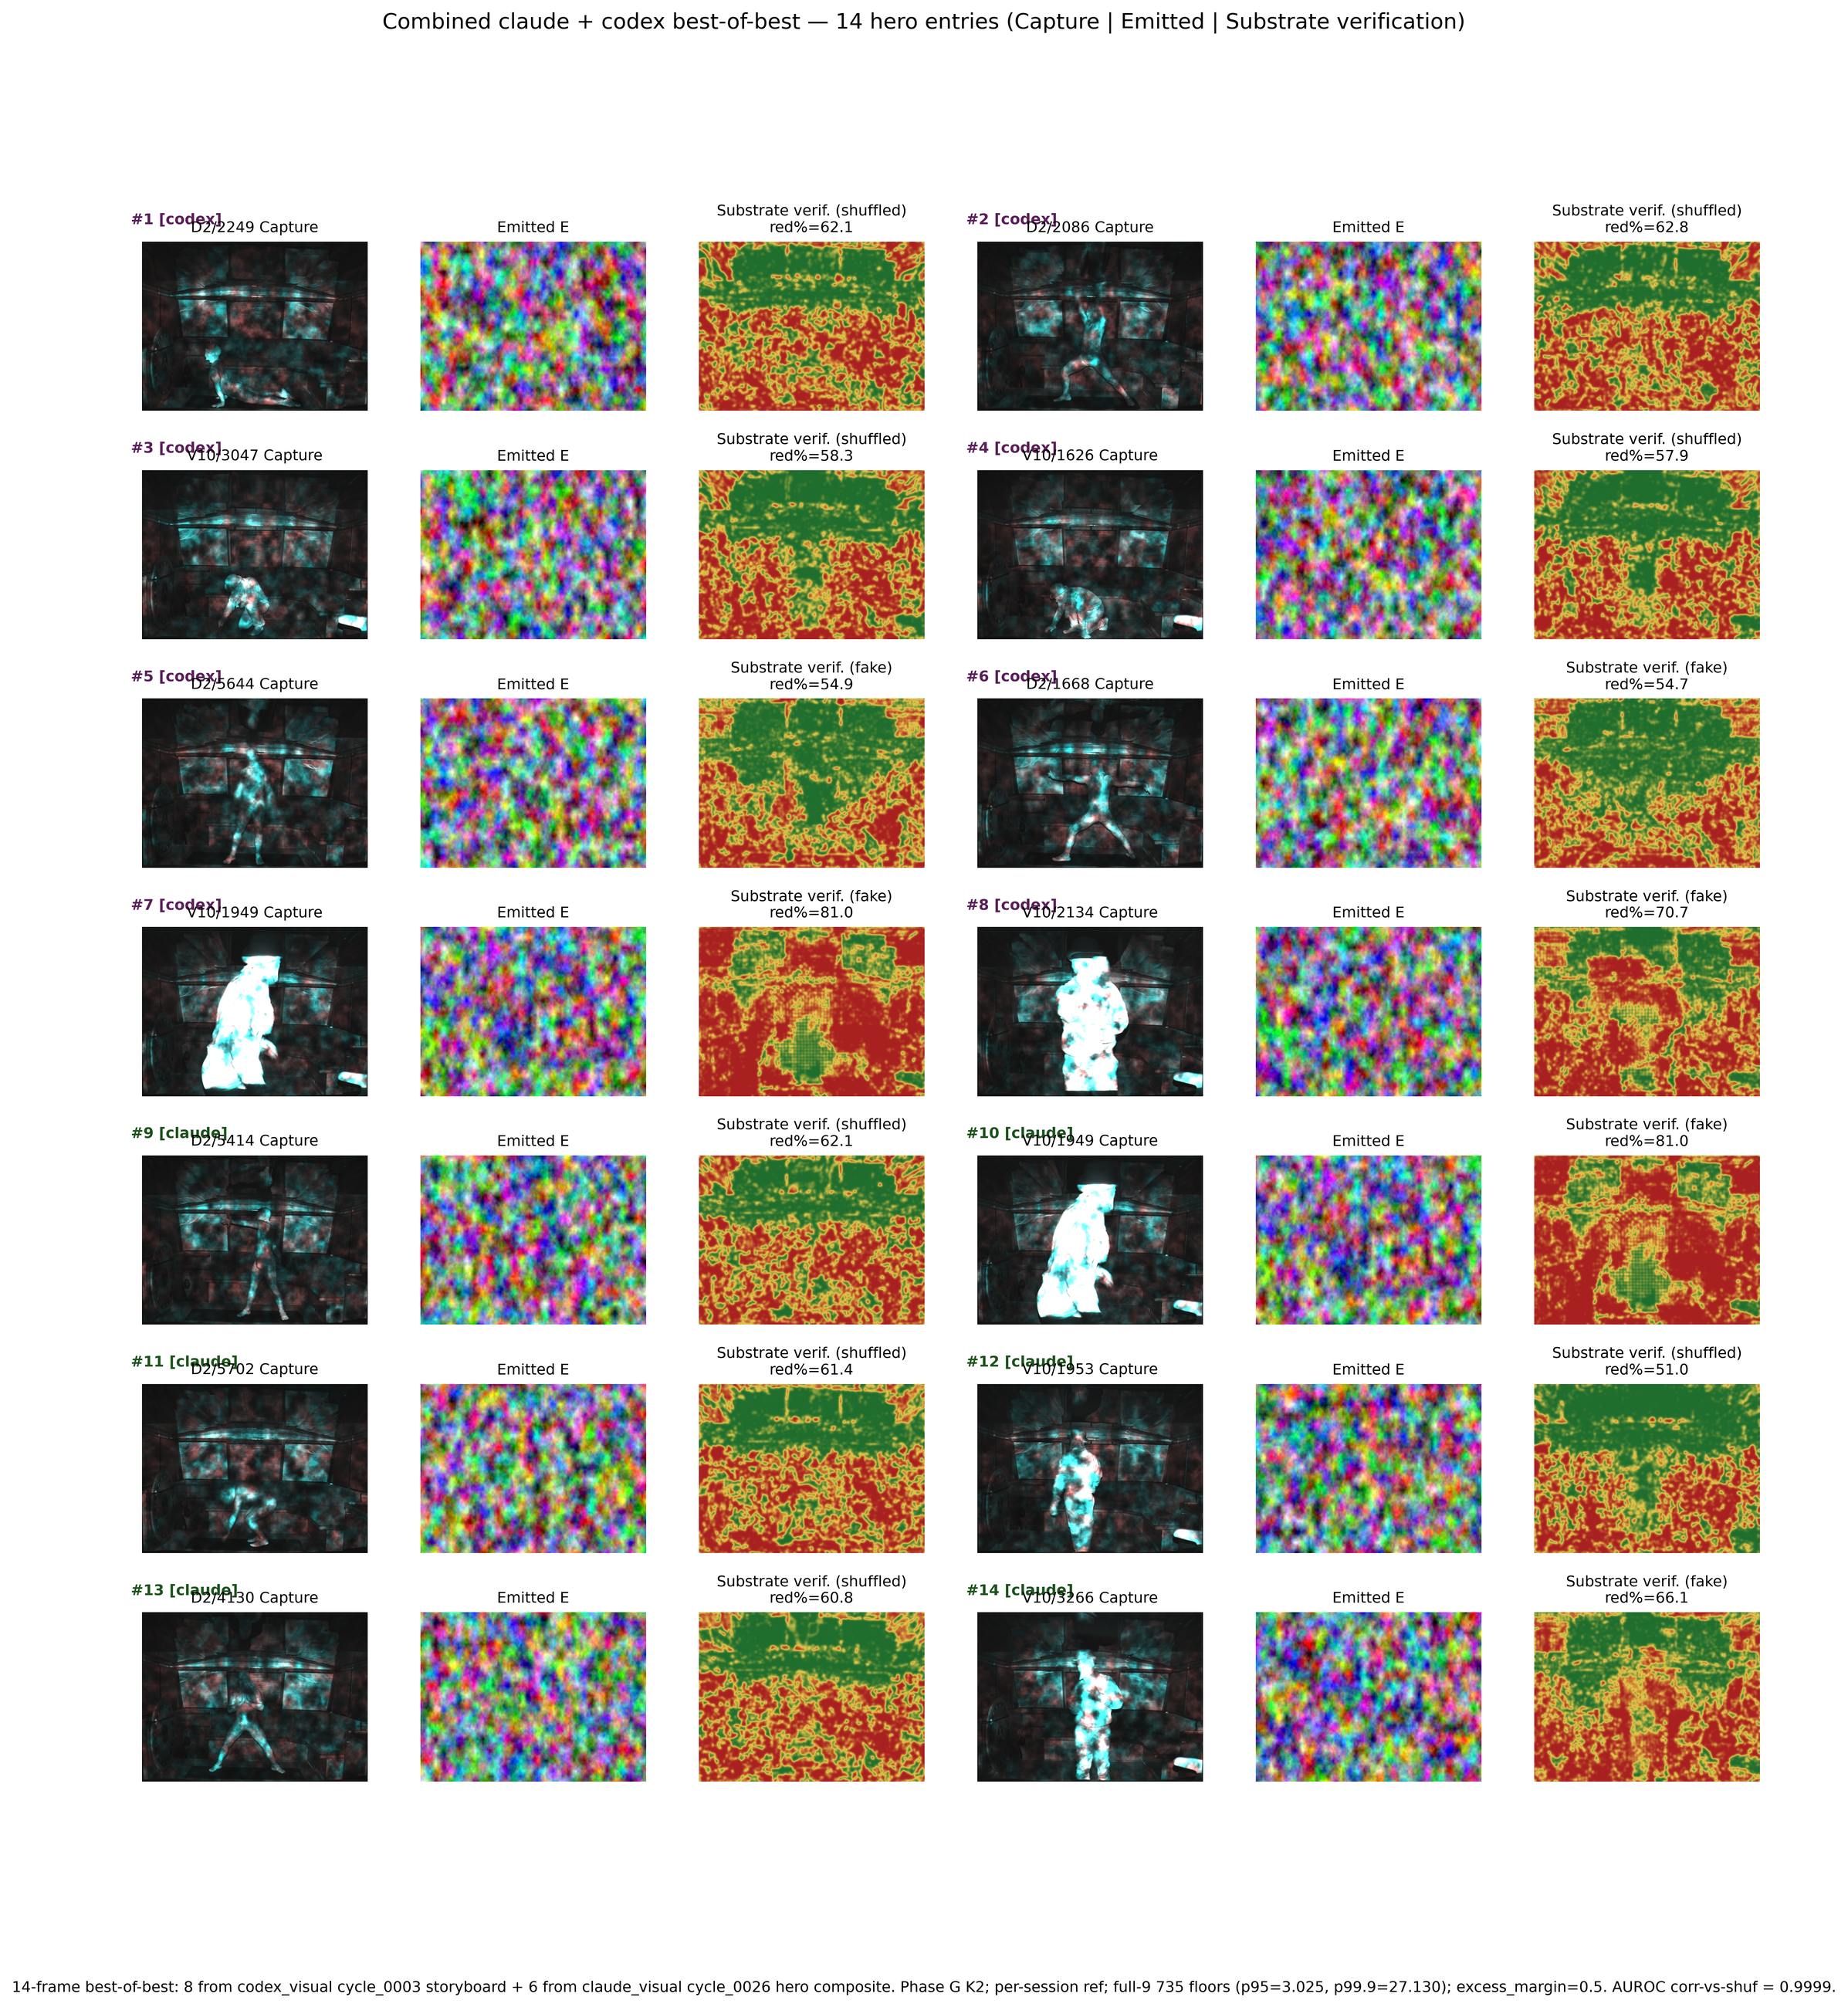
\includegraphics[width=\linewidth]{figures/fig_hero.png}
\caption{Substrate verification at a glance. Fourteen representative captures,
each shown as raw camera frame $C$, the emitted chain-coupled pattern $E$, and
the per-pixel substrate-verification map (Phase~G robust $z$-residual;
green~$=$~typical of a genuine chain-coupled capture, red~$=$~anomalous).
Real-correct frames render essentially uniformly green; substrate-altered
conditions (shuffled or synthetic $E$) render heavily red. All maps use a common
per-session reference (full-\num{9735}-frame p95/p99.9 floors, robust-$z$),
identical thresholds across all panels, and no per-frame normalization or body
suppression. This figure is illustrative; quantitative claims are reported in
\Cref{fig:roc} and \Cref{fig:zhist}.}
\label{fig:hero}
\end{figure}

\begin{figure}[tp]
\centering
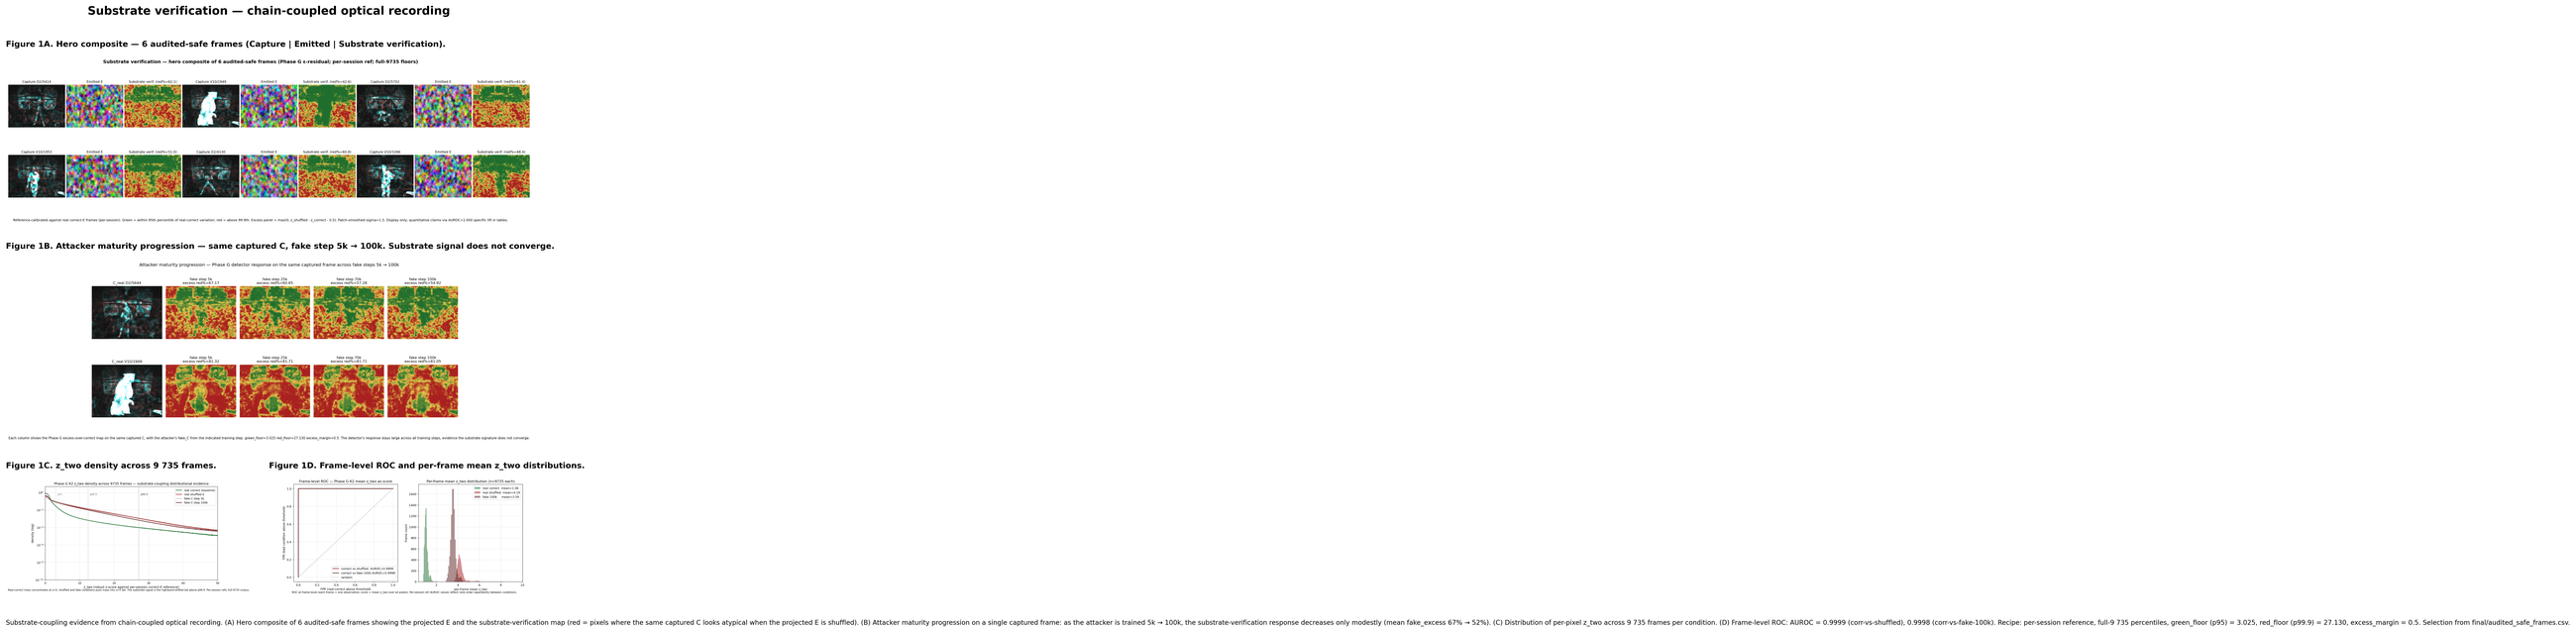
\includegraphics[width=\linewidth]{figures/fig_main_results.png}
\caption{Main result. (A)~Hero composite of substrate-verification maps for
genuine vs.\ substrate-altered captures. (B)~Attacker-maturity progression: the
same captured frame scored against synthetic emissions from adversary training
steps 5k--100k; the verification map stays strongly red at every maturity, i.e.\
the substrate signature does not converge as the attacker trains.
(C)~$z_{\text{two}}$ density across \num{9735} frames per condition.
(D)~Frame-level ROC and per-frame mean-$z$ distributions. Frame-level
AUROC~$=0.9999$ (correct vs.\ shuffled $E$) and AUROC~$=0.9998$ (correct vs.\
synthetic $E$ at step 100k) on this corpus. All maps use per-session references
and full-\num{9735} percentile floors with common thresholds within each paired
panel; AUROC values reflect rank-order separability between conditions on the
evaluated frame set, not a deployed operating point.}
\label{fig:main_results}
\end{figure}

\begin{figure}[t]
\centering
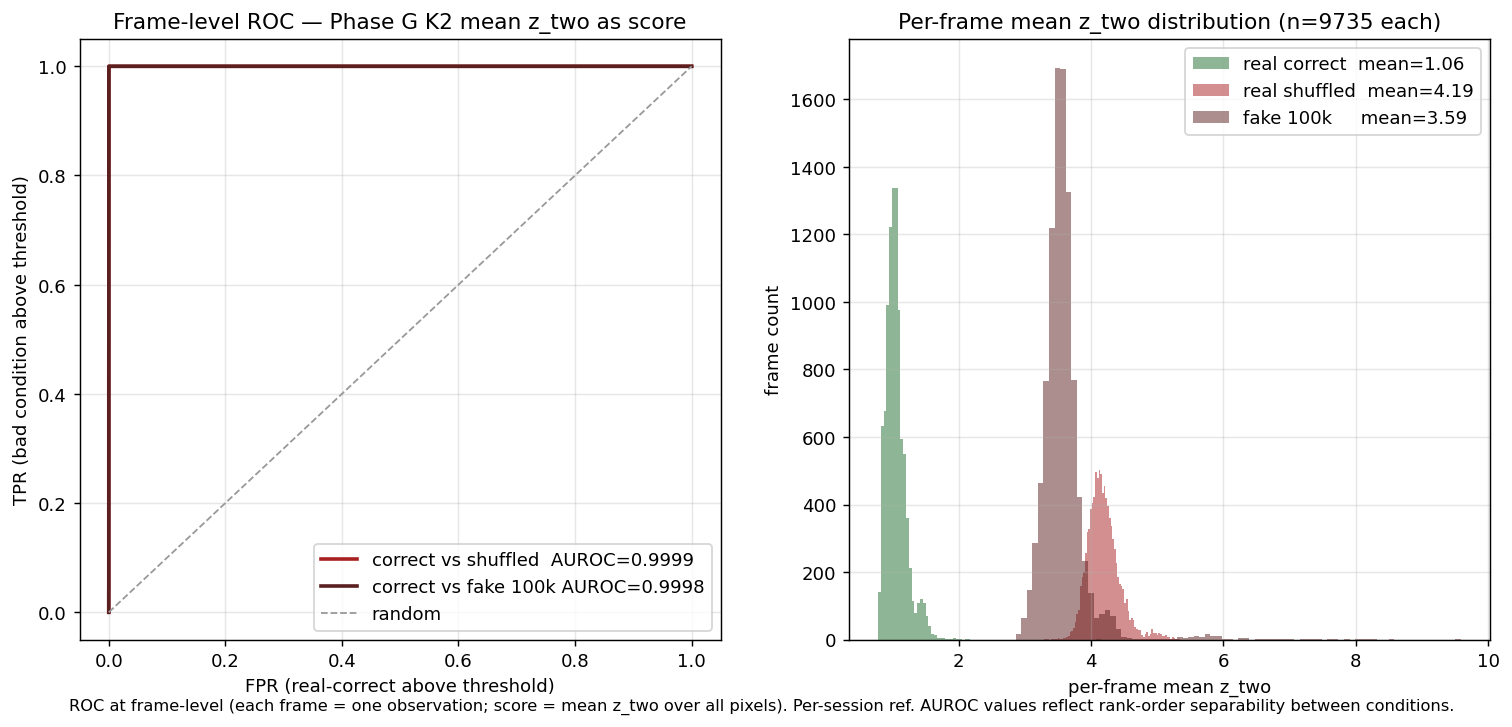
\includegraphics[width=\linewidth]{figures/fig_roc.png}
\caption{Frame-level separability. Left: ROC computed at the frame level, where
each frame is one observation and the score is the mean $z_{\text{two}}$ over all
pixels, giving AUROC = 0.9999 for correct vs.\ shuffled $E$ and AUROC = 0.9998
for correct vs.\ synthetic $E$ at training step \num{100000}. Right: per-frame
mean-$z_{\text{two}}$ distributions for the three conditions ($n=\num{9735}$
each), with the real-correct mode near $z=1.06$ and the shuffled ($4.19$) and
synthetic-\num{100000} ($3.59$) modes well separated from it. Per-session
reference; AUROC reflects rank-order separability between conditions on this
corpus, not a fixed-threshold field deployment.}
\label{fig:roc}
\end{figure}

\begin{figure}[t]
\centering
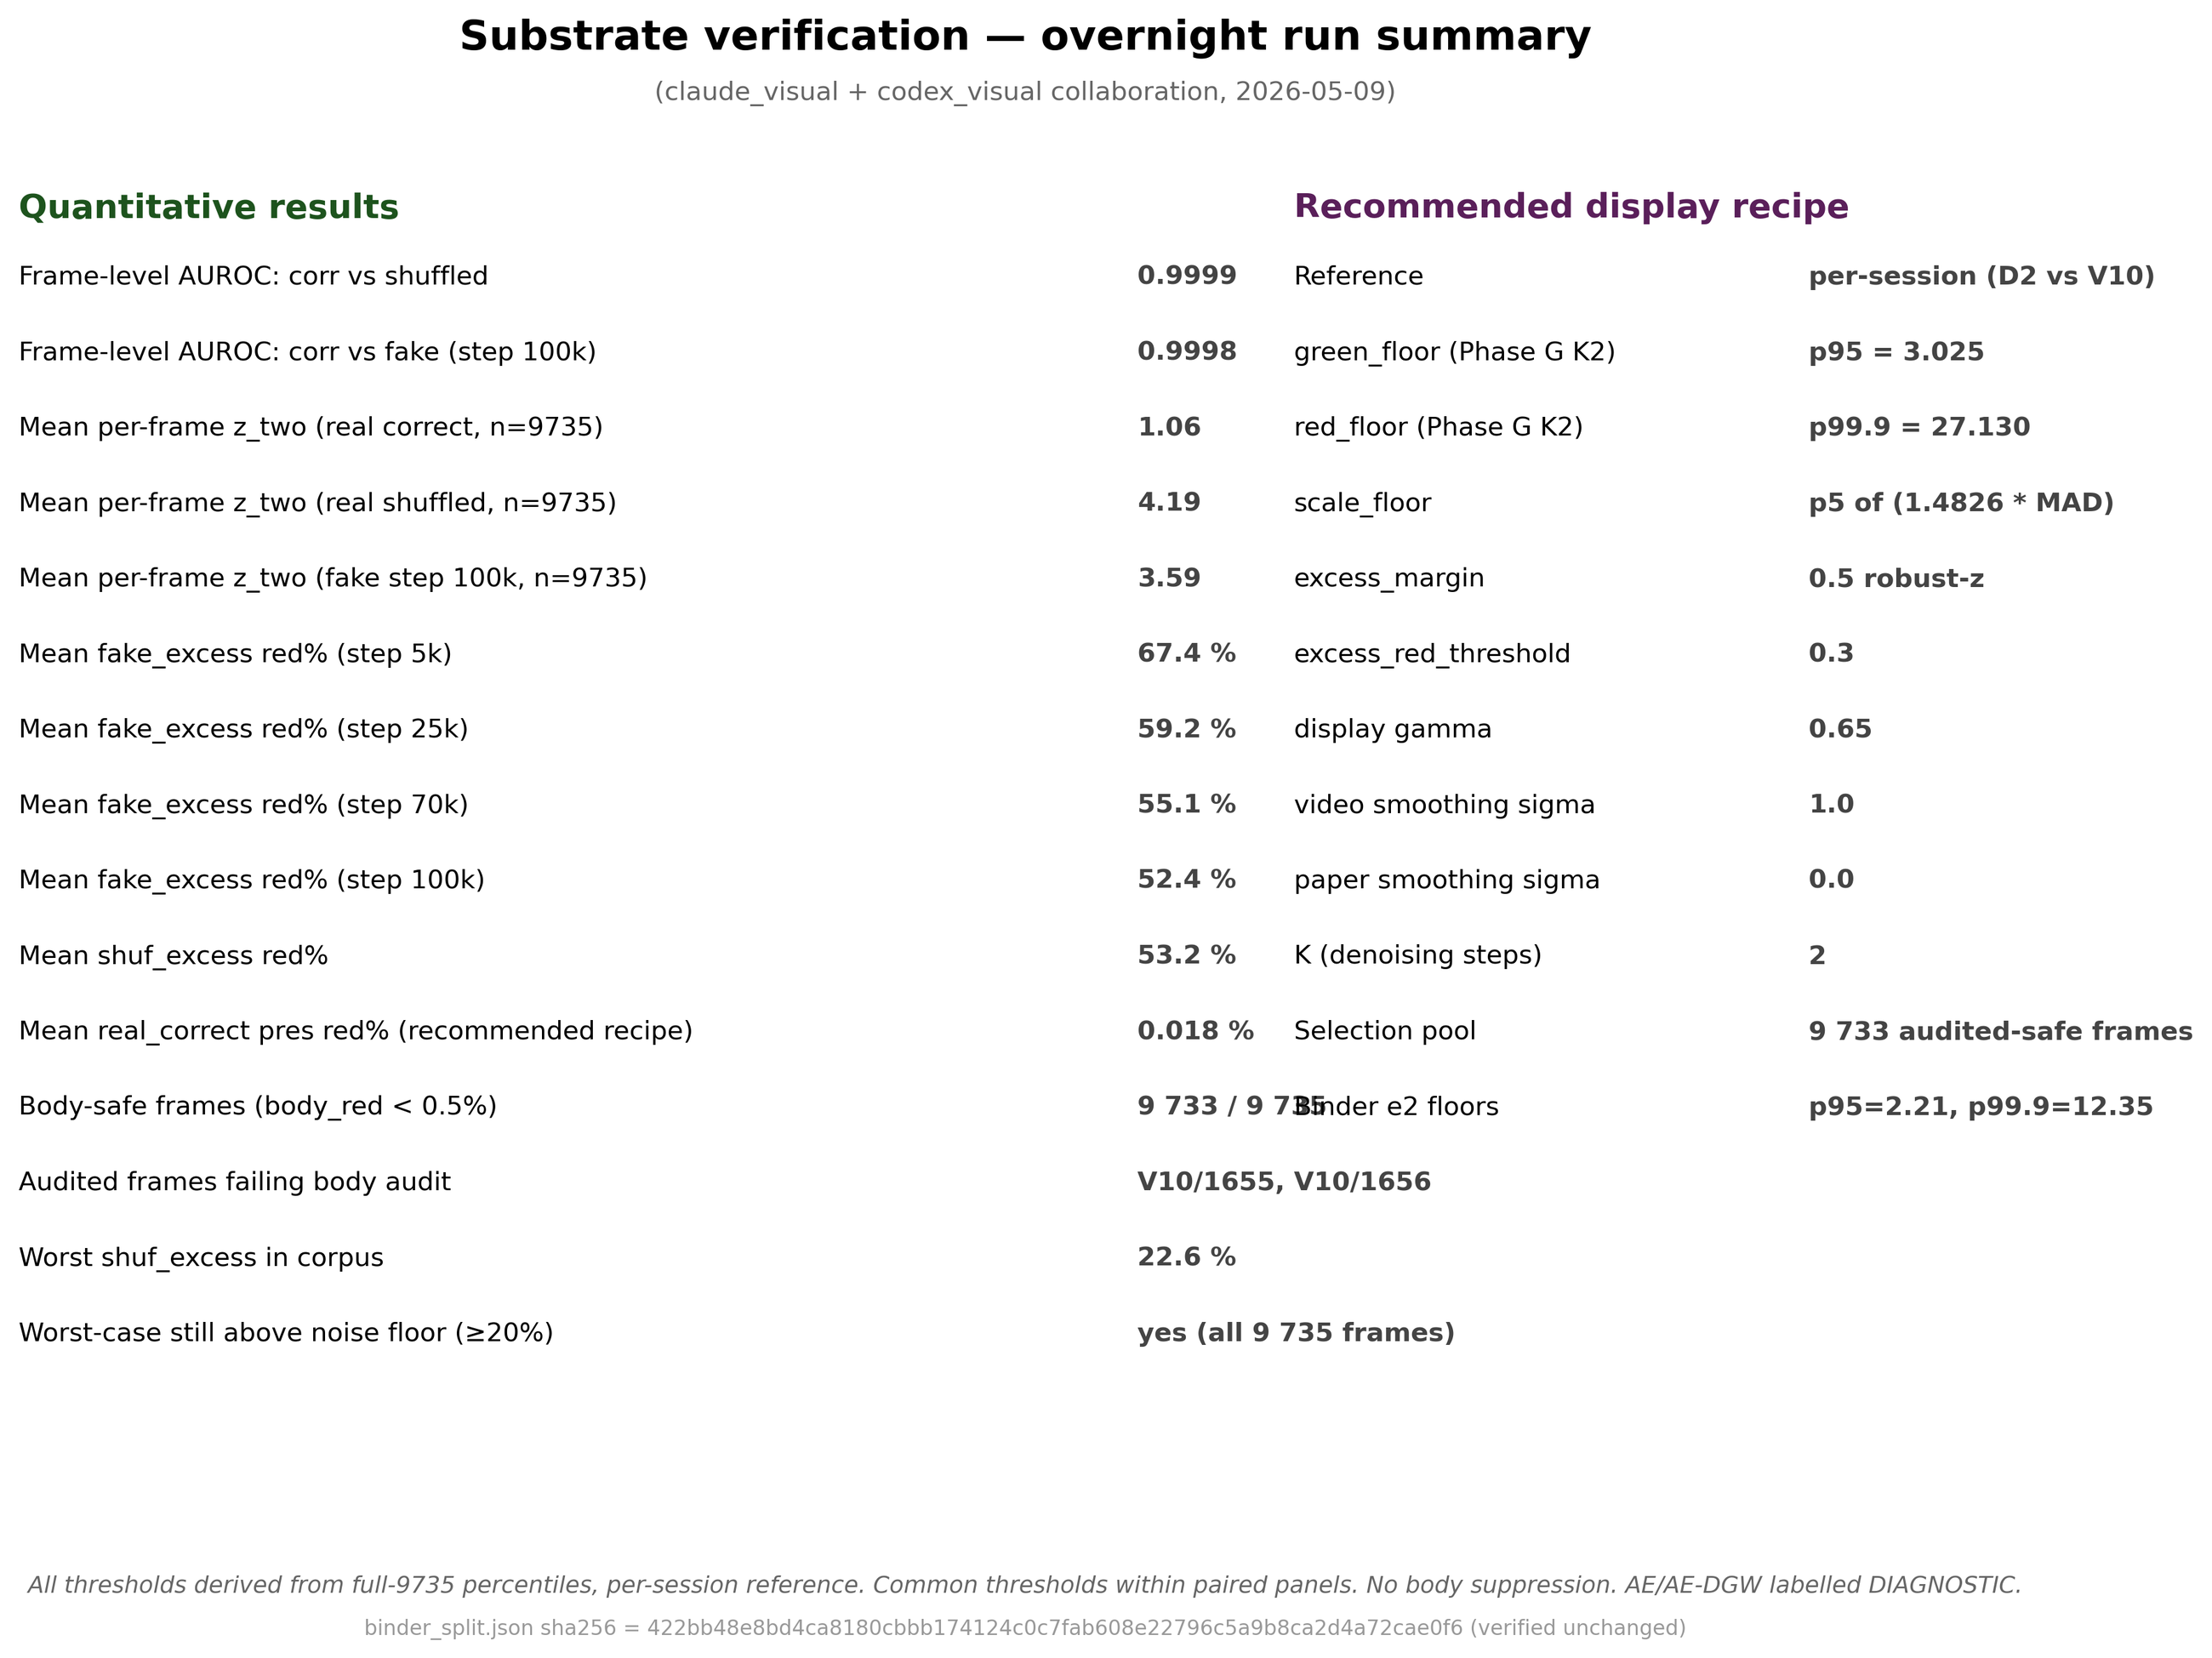
\includegraphics[width=\linewidth]{figures/fig_quant_table.png}
\caption{Quantitative summary and display recipe. Left: headline metrics ---
frame-level AUROC $0.9999$ (vs.\ shuffled) and $0.9998$ (vs.\ synthetic at step
\num{100000}); mean per-frame $z_{\text{two}}$ of $1.06$ (real-correct), $4.19$
(shuffled), $3.59$ (synthetic-\num{100000}); mean synthetic excess red\% declining
$67.4 \rightarrow 52.4$ across training steps \num{5000}\,$\rightarrow$\,\num{100000};
mean real-correct red\% $0.018\%$; \num{9733}/\num{9735} body-safe frames. Right:
the Phase~G K2 display recipe (green\_floor $=$ p95 $= 3.025$, red\_floor $=$ p99.9
$= 27.13$, scale\_floor $=$ p5 of $1.4826\cdot\mathrm{MAD}$, excess\_margin $0.5$,
$\gamma = 0.65$, $K=2$, per-session reference). All thresholds derived from
full-\num{9735} percentiles; common thresholds within paired panels; no body
suppression; AE/AE-DGW labeled DIAGNOSTIC.}
\label{fig:quant_table}
\end{figure}

\subsection{Same-rig cross-session and cross-protocol generalization}
\label{sec:results_main_generalization}

The main verifier is trained on real pairs from both sessions, so its held-out
blocks --- though strictly excluded from training with a \num{60}-frame guard
band and stride decimation --- are drawn from the same sessions seen in training.
To test whether the learned coupling transfers \emph{across} sessions, we run a
cross-session ablation: train the verifier on one session only and evaluate on
the entirely held-out other session. A D2-only verifier evaluated on held-out V10
achieves \textbf{AUROC = 1.0} for real-correct versus wrong/shuffled emissions,
and a V10-only verifier evaluated on held-out D2 likewise achieves
\textbf{AUROC = 1.0} (checkpoint step \num{100000}; both
$\text{real\_correct\_vs\_real\_shuffled} = 1.0$ and
$\text{real\_correct\_vs\_fake\_correct} = 1.0$). The verifier therefore does not
memorize a single session's emission statistics; the coupling it learns transfers
to a session it never saw during training.

This generalization is additionally cross-protocol. The two sessions were
recorded under structurally distinct chain transitions: D2 uses the v9 chain
(\texttt{ROW\_DOMAIN\_TAG} \texttt{b"TB:ROW:v9"}) and V10 uses the v10 chain
(\texttt{b"TB:ROW:v10"}), which additionally folds a \SI{32}{byte}
\texttt{ai\_payload\_root} committing AI-agent response frames into the state
transition $S_{t+1}$. A verifier trained on one protocol and evaluated on the
other still reaches AUROC = 1.0 on the real-correct-versus-wrong task, so the
result is a same-rig \emph{cross-protocol} generalization in addition to
cross-session. (Protocol version is confounded with session in this corpus ---
each protocol appears in exactly one session --- so we claim that verification
works across both versions, not that protocol version has no effect.)

\paragraph{Scope of the generalization claim.}
This result is strictly \emph{same-rig cross-session} (and same-rig
cross-protocol). It does \textbf{not} demonstrate cross-rig, cross-camera,
cross-projector, or cross-subject generalization; no such experiment exists in
this release, and whether the verifier generalizes beyond a single rig and a
single performer is untested. We are equally careful not to overstate uniformity within
the cross-session ablation. While the \emph{headline} real-correct-versus-shuffled
discrimination holds at AUROC = 1.0 out of distribution, other conditions degrade
when the verifier scores a session it was not trained on. The harder fake-pair
discrimination (fake\_correct vs.\ fake\_shuffled) drops out of distribution --- a
D2-only verifier on held-out V10 fakes falls to $0.8588$, versus $0.9295$ for the
combined verifier --- and the real-pair-versus-zero-$E$ AUROC also falls (e.g.\ a
D2-only verifier reaches $0.7221$ on V10). These drops indicate that part of the
verifier's coupling signal is session-specific. We therefore claim only that the
genuine-versus-anomalous separation transfers across same-rig sessions and
protocols; we do not claim uniform AUROC = 1.0 across all conditions, and we do
not claim robustness against the stronger F-A~v2 attacker, which is design-only
and not trained (see \Cref{sec:results_redteam}).

\subsection{Summary}
\label{sec:results_main_summary}

Three results anchor this section. First, the Phase~G verifier achieves
AUROC = 1.000 on held-out blocks of both sessions, with a tightly bounded
residual gap ($\Delta_{\text{wrong}} \approx +4\times10^{-3}$) that the
architecture- and data-matched shuffled control reduces to chance
(AUROC $\approx 0.5006$, $\Delta_{\text{wrong}} \approx 10^{-7}$), establishing
that the discrimination derives from genuine $C_t$--$E_t$ chain-coupling rather
than emission statistics or architecture. Second, at the frame level over the
full \num{9735}-frame corpus, the verifier reaches AUROC = 0.9999 against
shuffled emissions and AUROC = 0.9998 against F-A~v1 fakes at step \num{100000},
with real-correct frames rendering essentially green ($0.018\%$ mean red) and
anomalous conditions heavily red ($\sim$\,$51$--$53\%$). Third, the coupling
transfers same-rig across both sessions and both chain protocols at AUROC = 1.0
on the real-correct-versus-wrong task --- a generalization we bound explicitly to
same-rig scope, with documented out-of-distribution degradation on the harder
fake-pair and zero-$E$ conditions, and no claim beyond a single rig, two
sessions of one performer, and the single trained attacker F-A~v1.

\section{Results II: Adversarial Red-Team, Off-Body Coupling, and the Supervised Baseline}
\label{sec:results_redteam}

The within-session and same-rig cross-session results of \Cref{sec:results_main} establish that the trained Phase~G verifier separates genuine chain-coupled captures from temporally mispaired or shuffled emissions essentially without error. Those results, however, are constructed entirely from \emph{real} captures: the ``wrong-$E$'' negatives are real frames paired with the wrong emission. A verifier that only rejects mispaired-but-real captures says nothing about an adversary who synthesizes a forged capture $C_{\mathrm{fake}}$ explicitly conditioned on the real target emission $E_{\mathrm{target}}$. This section reports the system's behaviour against such a learned attacker, dissects \emph{where} in the image the discriminative signal lives, and characterizes a separately trained supervised baseline together with a fine-grained perturbation-sensitivity sweep. Throughout, two scope guards apply and are stated wherever a number is quoted: all evaluations are \emph{same-rig} (the single D2/V10 rig, one performer, two sessions) --- they do \emph{not} establish cross-rig, cross-camera, cross-projector, or cross-subject behaviour --- and the only \emph{trained} attacker is F-A~v1. The stronger F-A~v2 attacker is a design specification only; it is not trained, its trainer code does not exist, and nothing here should be read as a robustness claim against a strong or adaptive forger.

\subsection{Stage 0: a learned forger (F-A v1) is caught at every checkpoint}
\label{sec:redteam_stage0}

The red-team attacker, designated F-A~v1, is a learned editor that produces fake captures conditioned on a target emission. It is a 42.3M-parameter ControlNet-style \texttt{EditorControlNet}~\cite{zhang2023controlnet} built over a ConvNeXt-Tiny source encoder~\cite{liu2022convnext}: a $9$-channel spatial hint ($E_{\mathrm{target}}\,\|\,E_{\mathrm{source}}\,\|\,\Delta$) plus a $2$-channel coordinate grid is injected via zero-convolution adapters at four ConvNeXt scales. It was trained for \num{100000} steps ($\approx$\,\SI{28}{\hour}\,\SI{18}{\minute}; effective batch size $16$ on $8\times$ A100) against a pool of \emph{surrogate} binders (exp001c and e1-bf16 as training surrogates, with e2, e3r and an ablation family held out), so that it never received gradients from the Phase~G verifier itself. This separation is enforced as policy: Phase~G is reserved for final evaluation and is never used for attacker training, validation, checkpoint selection, or curriculum.

The headline Stage~0 result is that the Phase~G verifier rejects F-A~v1 forgeries at frame-level AUROC $=1.000$ for the real-correct vs.\ fake-correct contrast (genuine capture vs.\ forged capture, both paired with the correct $E_{\mathrm{target}}$), in \emph{both} sessions and at \emph{every} evaluated checkpoint --- steps 5k, 25k, 70k, and 100k --- on the standard held-out blocks (D2 $n=198$, V10 $n=200$). The attacker does not escape the verifier as it matures; its capacity to reproduce raw-capture realism plateaus while the verifier's separation remains saturated. We stress that this is a result about F-A~v1 specifically and is same-rig only.

A crucial nuance prevents a trivial reading of this result. One might suspect F-A~v1 is caught merely because it ignores the conditioning emission --- i.e.\ that it never learned to couple its output to $E_{\mathrm{target}}$ at all, so the verifier is simply detecting an absent hint. This is \emph{not} the case. By step 100k, F-A~v1 has demonstrably learned partial target-$E$ coupling: a forgery paired with its true $E_{\mathrm{target}}$ scores measurably better than the same forgery paired with a shuffled emission, with the fake-correct vs.\ fake-shuffled AUROC reaching $0.9927$ on D2 and $0.9295$ on V10. This coupling strengthens monotonically over training (D2: $0.609\!\to\!0.818\!\to\!0.967\!\to\!0.993$ across 5k/25k/70k/100k; V10: $0.585\!\to\!0.748\!\to\!0.870\!\to\!0.930$), confirming the editor is genuinely conditioning on $E$. F-A~v1 is therefore caught not for lacking emission structure, but for failing the \emph{real-capture conditional distribution}: its outputs do not reproduce the raw-capture realism, the fine chain-coupled statistics, and the source-leakage-free structure of genuine BayerRG8 frames. The held-out binder evaluation corroborates a \emph{soft} white-box specialization rather than catastrophic overfitting: the training-family binders score F-A~v1 output roughly \SI{3}{\decibel} better than held-out binders ($\approx$\,\SI{5}{\decibel} training target-gap vs.\ $\approx$\,\SI{1.7}{\decibel} held-out), yet the held-out family still ranks the true target first in $100\%$ of cases.

\paragraph{Probe saturation and decomposition deferral.}
We attempted to decompose \emph{why} the verifier separates F-A~v1 so cleanly by fitting logistic probes on Stage~0 diffusion features. Three feature families --- a Raw set (4 conditional MSEs), a Coupling set (3 contrasts), and their union (7 features) --- all saturate at AUROC $=1.000$ on the headline split (train on fakes at 5k/25k/70k, test on fakes at 100k; $n_{\mathrm{train}}=1272$, $n_{\mathrm{test}}=160$), and the saturation persists under leave-one-checkpoint-out cross-validation across all four checkpoints. Because every probe is perfect, F-A~v1 is simply too easy a target to support a meaningful feature-level decomposition; the deeper decomposition modes are deferred until a harder target (a trained F-A~v2) exists. We flag this as a deferral, not a completed analysis.

\paragraph{Cross-verifier robustness.}
A leave-one-session-out cross-verifier check confirms the forgeries remain detectable when scored by a verifier trained on only one session. The harder within-fake discrimination (fake-correct vs.\ fake-shuffled) degrades modestly out-of-distribution --- a D2-only verifier scores held-out V10 fakes at $0.8588$ (vs.\ $0.9295$ for the combined verifier), while a V10-only verifier holds D2 at $0.9927$ --- indicating that part of the verifier's coupling signal is session-specific and that F-A~v1 exploits that session-specific weakness. The real-pair coupling contrasts (real-correct vs.\ shuffled, real-correct vs.\ source) remain at AUROC $=1.000$ in all six (session $\times$ verifier) cells, so the core verification signal on genuine captures is intact across the ablation.

\subsection{Attacker non-convergence under continued training}
\label{sec:redteam_progression}

The visualization corpus (\num{9735} frames across D2 and V10) makes the non-convergence behaviour directly legible. Scoring a fixed captured frame against synthetic emissions drawn from successive attacker training steps, the substrate-verification \emph{excess} panel --- the per-pixel residual above the full-corpus p99.9 floor --- stays strongly red at every maturity. The mean synthetic excess-red area declines only modestly across training ($67.4\% \to 59.2\% \to 55.1\% \to 52.4\%$ at steps 5k/25k/70k/100k), while the genuine condition holds at a mean real-correct red area of $0.018\%$. \Cref{fig:attacker_progression} shows this progression for a single frame and reference: as the attacker matures its forgeries become marginally less anomalous, but the chain-coupled signature does not vanish. We emphasize that this is the F-A~v1 attacker; the result demonstrates that \emph{this} attacker does not converge to escape under continued training, not that no attacker could.

\begin{figure}[t]
\centering
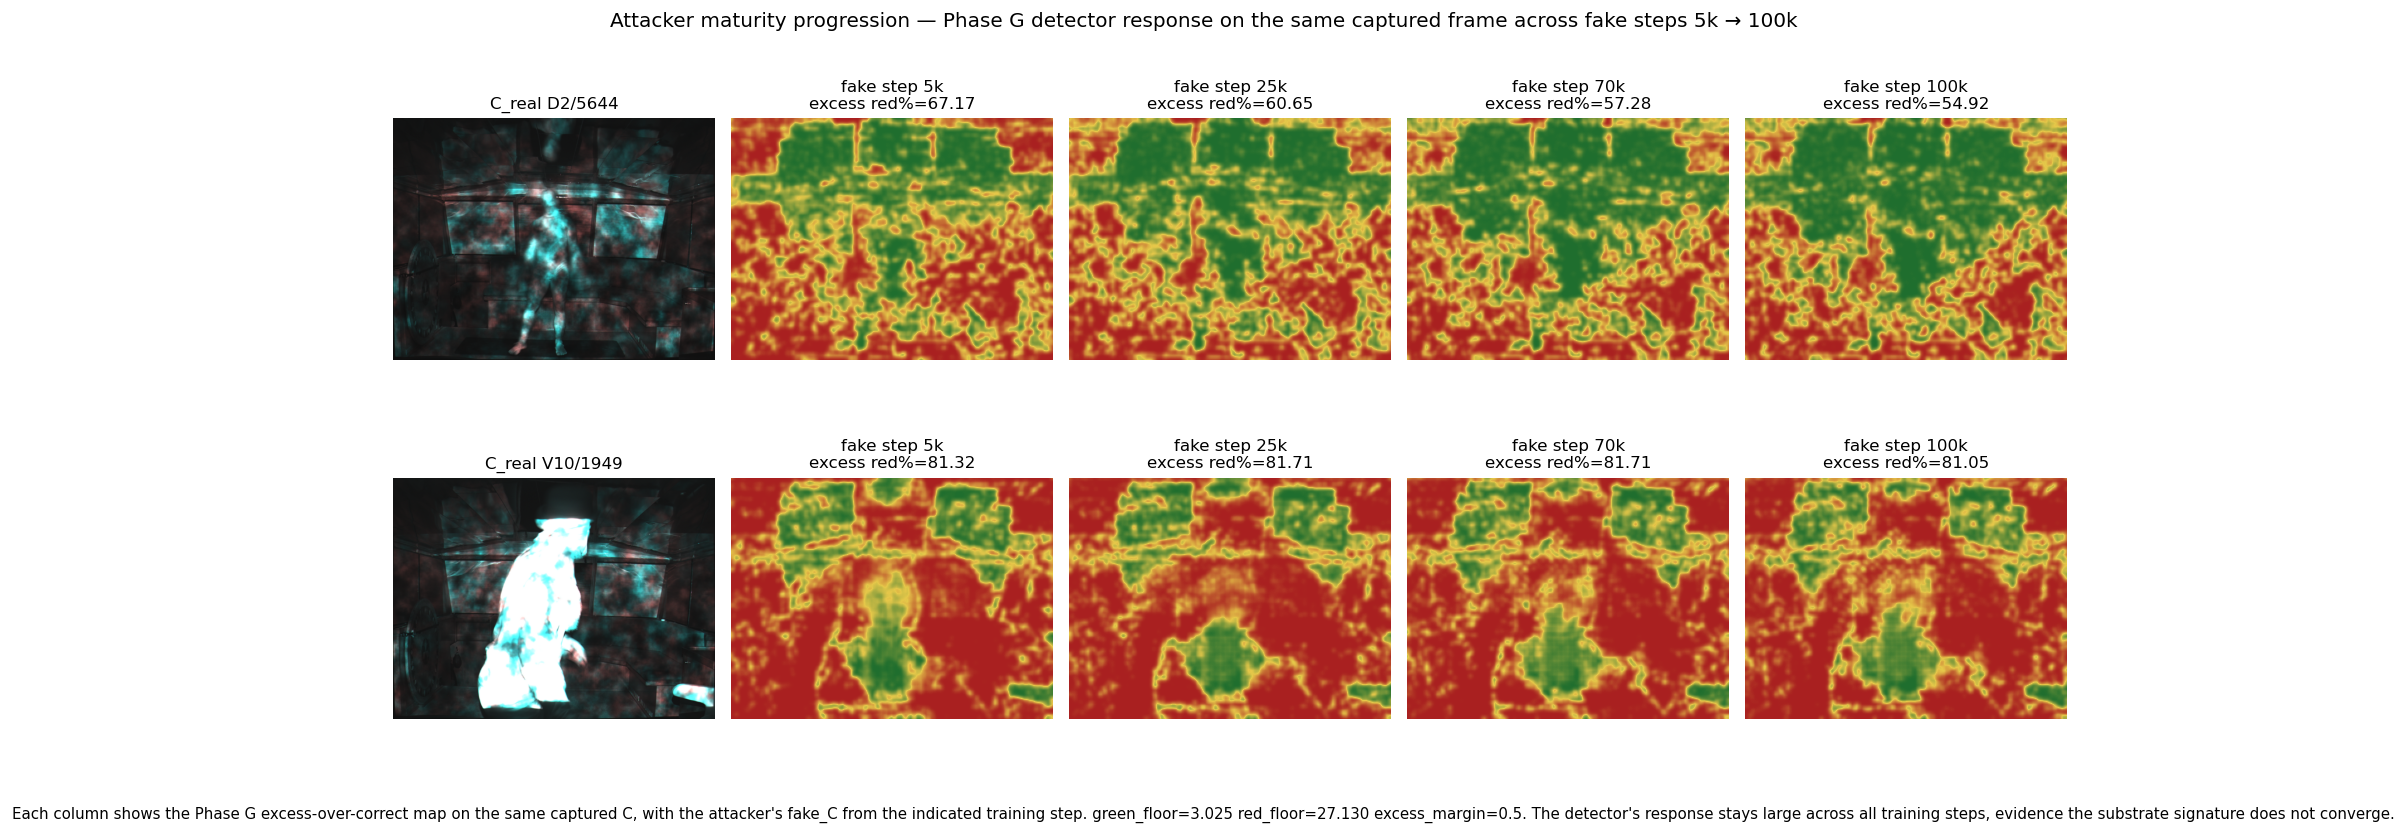
\includegraphics[width=\linewidth]{figures/fig_attacker_progression.png}
\caption{Attacker non-convergence (red-team). For a single captured frame $C$ and a single per-session reference, the synthetic emission is taken from F-A~v1 training steps 5k, 25k, 70k, and 100k. The substrate-verification excess panel remains strongly red at every step (mean excess red area $67.4 \to 59.2 \to 55.1 \to 52.4\%$), while the genuine condition holds at mean real-correct red area $0.018\%$. Residual coverage decreases only modestly as the attacker matures, indicating the chain-coupled signature does not converge under continued training of this attacker (F-A~v1). Green floor $=$ full-\num{9735} p95, red floor $=$ p99.9, excess margin $0.5$, common thresholds across all steps; no per-frame normalization.}
\label{fig:attacker_progression}
\end{figure}

\subsection{Where the discriminative signal lives: off-body, not on-body}
\label{sec:redteam_offbody}

A causal-ablation study asks which spatial region of the capture carries the signal the verifier uses to reject F-A~v1. The answer required correcting an early methodological error, and the correction inverted the conclusion; we report both readings because the inversion is itself instructive.

\paragraph{The variance-box reading and its failure.}
The first ablation masked the image into a ``body'' region and an ``off-body'' region using a variance-box heuristic (a $32\times32$ sliding-window variance with a p75 threshold, taking the largest vertically-extended connected component with a $10\%$ bounding-box expansion). Replacing the off-body region (condition E2, ``body only'') retained AUROC in the range $0.973$--$0.997$ on D2 and $0.983$--$0.995$ on V10, while replacing the body (condition E3, ``off-body only'') gave a lower $0.789$--$0.896$ (D2) / $0.926$--$0.977$ (V10). Read naively, this suggested ``body-region primacy.'' Visual inspection of the variance-box masks revealed the flaw: the heuristic ``body'' mask captured the body \emph{plus} adjacent high-variance non-body content --- projector patterns cast on the background, scene structure, and sensor frame edges. The variance box is a poor proxy for the subject silhouette precisely because the projected chain-coupled illumination makes static background regions high-variance.

\paragraph{The proper-segmentation reading inverts the conclusion.}
Re-running the identical ablation with true person silhouettes from a Mask R-CNN ResNet50-FPN segmenter \cite{he2017maskrcnn} (COCO weights; largest connected component with morphological close/open; \num{106} of \num{120} frames usable after dropping 14 pathological frames, an $11.7\%$ combined rate; per-session minimum 50/56) \emph{inverts} the finding. With proper segmentation, the body-only condition E2$_{\mathrm{seg}}$ collapses to AUROC $0.009$--$0.538$, while the off-body-only condition E3$_{\mathrm{seg}}$ reaches AUROC $=1.000$ across all twelve (session $\times$ condition) cells (the conditions being fake at 5k/25k/70k/100k, shuffled-$E$, and cross-session-$E$, for each of D2 and V10). All twelve cells classify as ``body alone insufficient'' under a decision tree frozen before the analysis. The paired hierarchical-bootstrap $\Delta$AUROC (E2$_{\mathrm{seg}}$ minus the variance-box E2) is large and its $95\%$ CI excludes zero in every cell --- e.g.\ D2 fake-5k $\Delta = -0.984$ $[-0.998, -0.964]$. An independent audit recomputed representative cells exactly (e.g.\ D2 fake-5k E2$\to$E2$_{\mathrm{seg}}$: $0.9924 \to 0.0088$) and returned a PASS verdict. \Cref{fig:segmentation} illustrates the ablation on a single frame.

\begin{figure}[t]
\centering
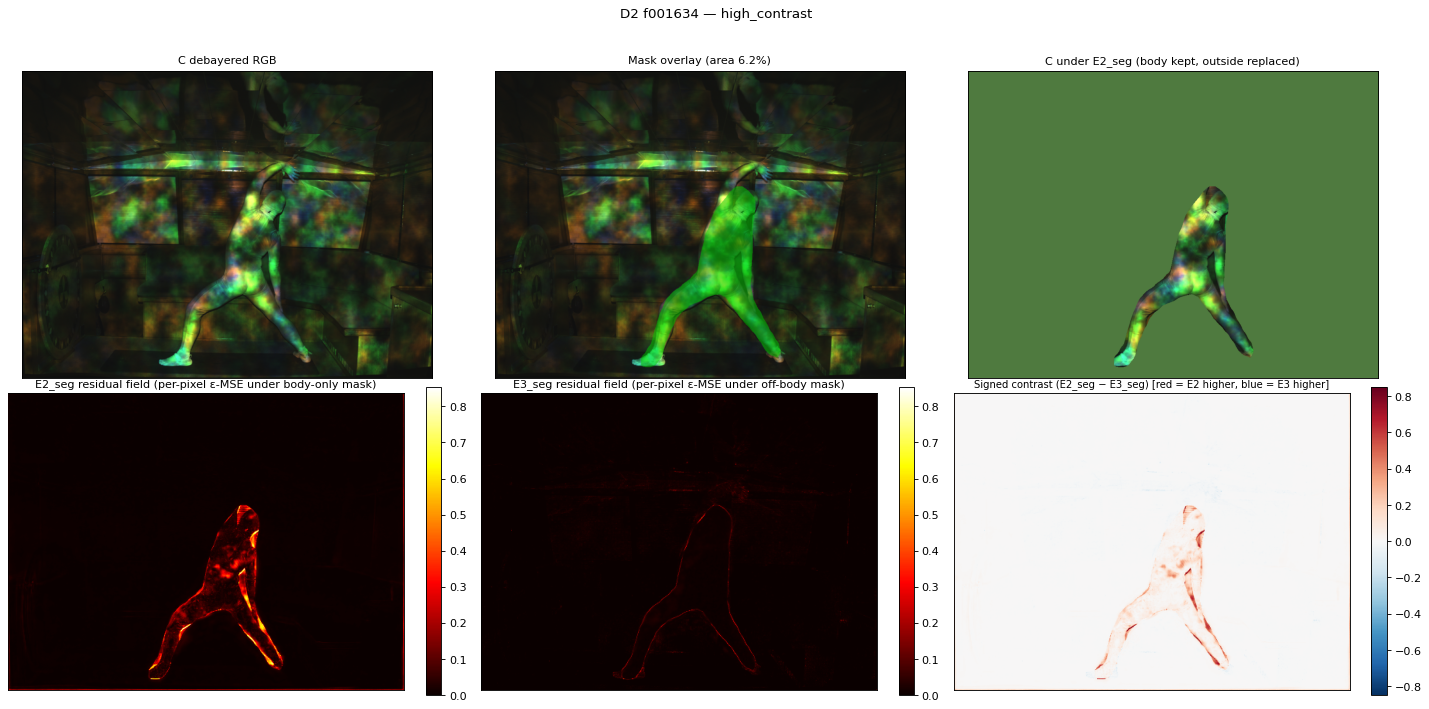
\includegraphics[width=\linewidth]{figures/fig_segmentation.png}
\caption{Where the discriminative signal lives: off-body, not on-body (segmentation ablation, frame D2 row 1634). Top row: debayered capture $C$, Mask R-CNN person mask (green overlay), and $C$ under the body-only ablation E2$_{\mathrm{seg}}$ (body kept, off-body replaced with per-channel inside-mask mean). Bottom row: E2$_{\mathrm{seg}}$ per-pixel residual field, E3$_{\mathrm{seg}}$ (off-body-only) residual field, and their signed contrast. Under proper Mask R-CNN segmentation, preserving only off-body content (E3$_{\mathrm{seg}}$) yields AUROC $=1.000$ across all conditions, while preserving only the body (E2$_{\mathrm{seg}}$) drops to chance or below (D2 fake AUROC $0.009$--$0.024$; $E$-perturbation $\approx 0.54$). This overturns an earlier variance-box reading and shows Phase~G's discrimination on F-A~v1 fakes resides in the off-body region. Scope caveat: analysis is over \num{106} usable frames and excludes the D2 block-2 supine-pose subset that Mask R-CNN segments unreliably ($11.7\%$ combined pathological rate; per-session minimum 50/56 usable).}
\label{fig:segmentation}
\end{figure}

\paragraph{Interpretation: likelihood overspread, not ``fakes look more real.''}
A striking feature of the inverted result is that the body-only AUROC falls \emph{below} chance on F-A~v1 fakes (D2 fakes $0.009$--$0.024$; V10 fakes $0.148$--$0.261$), meaning that under body-only masking, fake frames receive \emph{lower} anomaly scores than genuine frames. The correct framing is distribution-distance, not realism: F-A~v1 smooths body content, and its fake body region therefore lies in a region of Phase~G's conditional-likelihood landscape \emph{closer to the mode} than typical training-distribution real samples. This matches the overspread failure mode of likelihood-based out-of-distribution detection identified by Nalisnick et al.\ \cite{nalisnick2019} --- the reading most consistent with our measurements --- and we state it in those terms rather than as a claim that ``fakes look more real than real.'' The off-body reasoning is complementary: F-A~v1 does not perturb off-body content in a chain-coupled way, so the off-body region --- background scene, projection on static surfaces, and sensor frame edges --- retains the full discriminative chain-coupled signal and yields E3$_{\mathrm{seg}}$ AUROC $=1.000$.

\paragraph{The body signal is not absent --- it is at low spatial frequency.}
The ``body alone insufficient'' conclusion is specific to the $\lVert \hat{\epsilon}-\epsilon\rVert^2$ scoring function used by the verifier. The body region does carry a discriminative signal; it lives at low spatial frequencies that the residual-MSE score washes out under high-frequency dominance. Substituting a low-frequency scoring function (a Gaussian-blurred residual MSE, $\sigma = 4$) recovers body-only E2$_{\mathrm{seg}}$ AUROC $\approx 0.998$ (D2 $0.997$, V10 $0.998$), whereas $\lVert \hat{\epsilon}-\epsilon\rVert^2$ on the same masked region gives $\approx 0.30$--$0.41$ and a high-frequency residual is worse still ($\approx 0.21$--$0.32$). The correct claim is therefore narrow: residual-MSE body-only discrimination fails via OOD overspread, while a low-frequency body signal survives. We do not claim the body region is uninformative.

\paragraph{The relative-comparison test is unaffected and remains load-bearing.}
The absolute-MSE / OOD-overspread phenomenon above is orthogonal to a per-frame \emph{relative} chain-coupling test (EXP~6). In that test, each frame's correct emission is ranked against 50 random wrong emissions from the same session (with a $\pm 10$-frame temporal exclusion), giving 51 candidates per frame. The verifier ranks the correct $E$ first in $100\%$ of frames (top-1 $=1.000$, top-5 $=1.000$, mean rank $1.00$; $n=120$, D2$=60$ / V10$=60$). Because this test compares candidate emissions for a fixed capture rather than comparing absolute residual magnitudes across frames, it is immune to the overspread artifact and remains the load-bearing demonstration that Phase~G's signal is genuine chain-coupling.

\paragraph{Multi-method agreement on genuine captures.}
As a cross-check, the verifier-tier residuals can be compared against diagnostic representations on genuine frames (\Cref{fig:multimethod}). Two verifier-tier methods (Phase~G K2 and a binder residual) and two autoencoder-based diagnostic taps (AE-64f and AE-DGW) all report typical (green) residual on real-correct frames. The autoencoder methods are reported for cross-checking only and are explicitly labeled \textsc{Diagnostic}, not verifier-tier, because they exhibit weak coupling-specificity; quantitative claims rest on the per-method AUROC tables, not on the clipped display.

\subsection{A supervised baseline (Phase H): coarse-aware, fine-blind}
\label{sec:redteam_phaseh}

To contextualize the diffusion verifier against a conventional discriminative approach, we trained a small supervised CNN classifier (Phase~H) on $(C,E)$ input with real captures as positives and shuffled / perturbed-XOF captures as negatives. Phase~H is a coarse baseline with a known data-augmentation limitation, not a production verifier, and we report it as such.

\paragraph{It is emission-aware for coarse contrasts.}
An $E$-usage ablation on the converged checkpoint confirms Phase~H genuinely uses the emission for coarse discrimination: AUROC(target vs.\ shuffled) $=1.0000$ and AUROC(target vs.\ source) $=1.0000$ in both sessions (mean per-frame logits, D2: target $+4.897$, shuffled $-13.674$, source $-13.675$). The classifier cleanly separates the target emission from substantially different emissions. We note that AUROC(target vs.\ zero-$E$) reads $0.0$, but this is an out-of-distribution artifact --- zero-$E$ was never observed in training, and its mean logit ($+35.6$) sits far outside the in-distribution range --- so we do not cite it as a failure; the conclusions rest on the in-distribution target-vs-shuffled and target-vs-source contrasts.

\paragraph{It is blind to fine XOF perturbations.}
The same classifier does not resolve fine emission perturbations: Type~1 global BLAKE3-XOF bit-flips and Type~3 spatially-localized bit-flips score approximately at chance, while a Type~6 full-emission replacement is separated perfectly (AUROC $=1.0$). The canonical framing, which we adopt verbatim, is that ``the supervised CNN baseline is $E$-aware, but its learned evidence is coarse. It separates target emissions from substantially different emissions, but does not resolve fine XOF-level perturbations in this training regime.'' The distinction is one of contrast scale and perturbation family, not of abstract granularity.

\paragraph{The blindness is partly a label-locking artifact.}
A sampling audit identifies the proximate cause as per-frame label-locking: the epoch seed is fixed once at dataset construction and never refreshed, so each (session, row, index) tuple is permanently locked to a single role (positive, shuffled, or perturbed-with-a-specific-label). With 28 train-pool perturbation labels and a dataset of \num{2679} samples per epoch (positive $49.6\%$, shuffled $25.4\%$, perturbed $25.0\%$), only $\approx$\,17--33 unique frames back each perturbation label. Roughly half of all frames are never shown as a negative, and the model learns a per-frame label rather than per-condition discrimination. The recommended fix is to re-derive the epoch seed per epoch so frames rotate through all roles. We therefore attribute Phase~H's fine-blindness to the perturbation family combined with this augmentation deficiency, not to an intrinsic granularity ceiling.

\subsection{Item 1: fine-grained perturbation sensitivity of the diffusion verifier}
\label{sec:redteam_item1}

Finally, we probed whether the trained Phase~G diffusion verifier itself --- the load-bearing method --- exhibits the same coarse/fine structure. The Item~1 sweep ran 53 conditions $\times$ 2 sessions (D2 $n=198$, V10 $n=200$) against the main checkpoint at the five fixed eval timesteps with $K=4$ noise samples, augmenting the baseline conditions with 35 extended XOF perturbations. Per-condition AUROCs for the extended families are computed directly from the raw evaluation arrays; the shipped summary file covers only the baseline conditions.

The sweep is exploratory: per-condition AUROCs are reported descriptively, without multiple-comparisons correction across the 53 conditions; saturated separations (AUROC $=1.000$) lie far beyond any plausible multiplicity artifact, while near-chance values are read only as ``not detected,'' never as evidence of absence. The verifier confirms the same fine/coarse divide observed in Phase~H, now with a graded, frequency-dependent structure:
\begin{itemize}
  \item \textbf{Fine perturbations are near-chance.} Type~1 global bit-flips rise only at very large flip counts (D2: $k{=}1$ AUROC $0.503 \to k{=}4096$ AUROC $0.599$; V10: $0.503 \to 0.583$). Type~3 localized $8\times8$-region bit-flips in octave 2 stay near chance even at $k{=}256$ (D2 $0.506$, V10 $0.505$). We explicitly do \emph{not} claim Phase~G detects small-$k$ Type~1 or fine Type~3 flips.
  \item \textbf{Sensitivity is octave/persistence-dependent.} Low-frequency octave-0 perturbations are detectable while high-frequency octave-3 perturbations remain near chance: Type~2 oct-0 $k{=}64$ reaches $\approx 0.57$--$0.59$ vs.\ $\approx 0.503$ for oct-3; a Type~4 octave swap is perfect for oct-0 ($1.000$) but only $\approx 0.57$ for oct-3.
  \item \textbf{Gross perturbations are perfectly separable.} Full-emission replacement (Type~6), the wrong-$E$ offset, the octave-0 swap (Type~4), and the R-channel swap (Type~5) all reach AUROC $=1.000$ in both sessions; a B-channel swap is high but imperfect ($0.987$ D2 / $0.970$ V10) and is reported distinctly.
\end{itemize}
A renderer-calibration check passes (the Type~6 calibration condition matches the existing wrong-$E$ condition to $\approx 5\times 10^{-6}$ per-frame MSE), confirming the XOF$\to$render pipeline is deterministic and reproduces the baseline wrong-$E$ renderer. These sensitivities should be interpreted against the rendered-emission difference $\Delta E$: a very small XOF bit-flip may fall below the optical-relevance threshold, so its near-chance AUROC likely reflects an emission that is barely changed at the projector rather than a verifier deficiency. The graded result is consistent with the optical low-pass characterization of the substrate: the chain-coupled signal that survives projection and capture is the emission's low-frequency structure, and that is exactly where verifier sensitivity is highest.

\section{Discussion: Scope, Limitations \& Future Work}\label{sec:discussion}

The results in the preceding sections establish a clear and, we believe, defensible claim: on this rig, real chain-coupled captures carry a learnable physical signature that a diffusion verifier can use to separate genuine recordings from substrate-altered or forged ones with near-perfect rank-order separability (frame-level AUROC $=0.9999$ against shuffled emissions and $=0.9998$ against the F-A v1 synthetic forger at training step \num{100000}). It is precisely because that headline is strong that this section is devoted to stating, in detail, what the evidence does \emph{not} show. The PolieBotics programme treats anti-overclaim as a methodological discipline rather than a disclaimer, and the limitations below are integral to the result, not caveats appended to it.

\subsection{Scope: same-rig, two-session, single-subject}\label{sec:discussion:scope}

The single most important boundary on every quantitative claim in this report is that all of it is \emph{same-rig}. The corpus comprises exactly two capture sessions recorded on one projector--camera apparatus with one human performer: D2 (\texttt{cittadel\_first\_human}, \num{5992} chain rows) and V10 (\texttt{cittadel\_v10\_mainnet\_improv}, \num{3743} chain rows), for a combined \num{9735} frames. Both sessions use the same Sony IMX540 sensor delivering \SI{8}{bit} BayerRG8, the same projector, and the same physical scene geometry. Every figure in this report --- the hero substrate maps (\Cref{fig:hero}), the per-frame decision triples (\Cref{fig:overview}), the ROC and $z$-score distributions (\Cref{fig:roc,fig:zhist,fig:ecdf}), the segmentation ablation (\Cref{fig:segmentation}), and the multi-method agreement panel (\Cref{fig:multimethod}) --- is computed on this same two-session corpus.

Within that boundary the generalization we \emph{can} demonstrate is two-fold and genuine. First, it is cross-session: a verifier trained only on D2 and evaluated on held-out V10 reaches AUROC $=1.0$ for real-correct-$E$ versus wrong/shuffled-$E$, and the symmetric V10-only $\rightarrow$ D2 ablation likewise reaches AUROC $=1.0$. Second, it is cross-protocol: D2 was recorded under the v9 chain (\texttt{ROW\_DOMAIN\_TAG} \texttt{b"TB:ROW:v9"}) and V10 under the structurally distinct v10 chain (\texttt{b"TB:ROW:v10"}, which additionally folds in a \SI{32}{byte} \texttt{ai\_payload\_root} committing AI-agent response frames), so a verifier that performs across both sessions is, by construction, performing across both protocol versions on the same rig.

What these ablations do \emph{not} establish must be stated without hedging. They do not demonstrate cross-rig generalization, nor cross-camera, cross-projector, or cross-subject generalization. The held-out blocks in the \emph{main} verifier's evaluation are drawn from the same two sessions used in training, so the headline AUROC $=1.000$ is a within-session (same-rig) measurement, separated from the training rows only by held-out blocks with a 60-frame guard band and stride decimation; the single-session ablations above are the exception, and they constitute the cross-session evidence. A reader should therefore not infer that a Phase G checkpoint trained here would verify recordings made on a different apparatus, with a different sensor or projector, or featuring a different subject. We regard cross-rig validation as the central open empirical question of the programme, not a foregone conclusion.

The small number of sessions compounds this. With $n=2$ sessions and one operator, the dataset cannot disentangle session-to-session variation from rig-to-rig or subject-to-subject variation, and there is direct evidence that part of the learned coupling signal is session-specific. One mitigating detail is worth recording: the performer's appearance differs substantially between the sessions (a different costume and mask in each --- yoga attire in D2, an improv costume in V10), so the cross-session transfer already spans a change in the subject's visual appearance. It remains one performer on one rig, and we do not count this as cross-subject evidence. While the headline real-versus-shuffled discrimination holds at AUROC $=1.0$ out-of-distribution, the harder fake-pair discrimination degrades when a single-session verifier scores the held-out session: the D2-only verifier's discrimination of F-A v1 fakes on V10 drops to AUROC $=0.8588$, and real-pair-versus-zero-$E$ coupling also falls out-of-distribution (for example, the D2-only verifier on V10 reaches AUROC $=0.7221$). These drops do not represent an attacker escape --- F-A v1 remains caught --- but they show that not all of the verifier's coupling evidence transfers cleanly across sessions, which is exactly the kind of effect that more sessions and more rigs are needed to characterize.

\subsection{The strong adaptive attacker is future work}\label{sec:discussion:adaptive}

The red-team evidence in this report establishes robustness against \emph{one} concrete learned forger: F-A v1, a 42.3M-parameter ControlNet-style editor (EditorControlNet over a ConvNeXt-Tiny source encoder) trained for \num{100000} steps to produce fake captures $C_\text{fake}$ conditioned on a target emission $E_\text{target}$. Phase G catches F-A v1 at real-versus-fake AUROC $=1.0$ at every evaluated checkpoint (5k, 25k, 70k, 100k) in both sessions, and the catch is not an artifact of the forger ignoring the target emission: by step \num{100000} F-A v1 has learned measurable target-$E$ coupling (fake-correct versus fake-shuffled AUROC rising to $0.9927$ on D2 and $0.9295$ on V10), so it is caught for failing the real-capture conditional distribution, raw-capture realism, and source leakage --- not for lacking $E$-structure. \Cref{fig:attacker_progression} shows the operational consequence: the substrate-verification excess panel stays strongly red as the attacker matures (excess red declining only modestly, $67.4\% \rightarrow 52.4\%$ across steps 5k$\rightarrow$100k), while the genuine condition holds at mean real-red $0.018\%$, indicating non-convergence of the forgery under continued training of \emph{this} attacker.

We must be emphatic about the limit of that claim. The stronger adaptive attacker, F-A v2 --- a forger trained against fresh binder surrogates with a wider 17-channel hint stack and full-resolution $C_\text{fake}$ output --- exists only as a design specification. It is \textbf{not trained and not implemented}; the trainer code does not exist. Consequently, \emph{nothing in this report establishes robustness against a strong or adaptive attacker.} The F-A v1 result should be read as evidence that the substrate signature withstood one competent, non-trivial learned forger --- not as evidence that the signature is unforgeable. The off-body finding (\Cref{fig:segmentation}) sharpens this point by localizing the discriminative signal: under proper Mask R-CNN segmentation, preserving only the off-body region (E3$_{\mathrm{seg}}$) yields AUROC $=1.000$ across all twelve session-by-condition cells, while preserving only the body (E2$_{\mathrm{seg}}$) collapses to AUROC $0.009$--$0.538$. F-A v1 smooths body content and does not perturb off-body content in a chain-coupled way; whether F-A v2 can be trained to perturb off-body regions in a chain-coupled manner that matches the target emission is an open design target, not a result. The body-region collapse itself must be stated carefully, in distribution-distance / likelihood-overspread terms \cite{nalisnick2019}: under the $\epsilon$-prediction MSE score, F-A v1 fake body content lies nearer the verifier's conditional-likelihood mode than training-distribution real samples. The body signal is not absent --- it survives at low spatial frequencies (a Gaussian-blurred residual MSE at $\sigma=4$ retains E2$_{\mathrm{seg}}$ AUROC $\approx 0.998$) but is washed out by the high-frequency-dominated $\epsilon$-MSE. We deliberately avoid the phrasing ``fakes look more real than real''; the correct statement is that the absolute-MSE body-only discrimination fails via OOD overspread, while the relative-comparison chain-coupling test (per-frame top-1 $=100\%$ across 120 frames) is orthogonal to that phenomenon and remains the load-bearing chain-coupling demonstration.

\subsection{Supervised baseline blindness to fine perturbations}\label{sec:discussion:baseline}

A second limitation concerns the granularity of the evidence the verifiers actually use. The supervised CNN baseline (Phase H) is \emph{E-aware} for coarse contrasts --- it separates target emissions from shuffled and source emissions at AUROC $=1.0$ in both sessions --- but its learned evidence is coarse: it does not resolve fine XOF-level perturbations in this training regime. Concretely, Phase H is near chance on Type 1 global single-to-few-bit flips and Type 3 spatially localized bit-flips, while full emission replacement (Type 6) is trivially separable at AUROC $=1.0$. We attribute this in part to a data-augmentation limitation rather than a fundamental granularity ceiling: a sampling audit revealed per-frame label-locking, in which the \texttt{epoch\_seed} is fixed once at dataset construction and never refreshed, permanently locking each \texttt{(session, row, idx)} tuple to a single role and yielding only $\sim$17--33 unique frames per perturbation label across 28 train-pool labels. Roughly half of all frames are never shown as a negative. Phase H is therefore best characterized as a fast supervised \emph{coarse} baseline with a known and fixable augmentation deficiency, not as a production verifier.

Crucially, the same fine-perturbation structure appears in the trained Phase G diffusion verifier itself, which is independent of the label-locking artifact. An extended sensitivity evaluation (53 conditions $\times$ 2 sessions) shows Phase G's response is graded and octave/persistence-dependent. Small-$k$ Type 1 global flips are near chance (D2 $k{=}1$ AUROC $\approx 0.503$, rising only to $\approx 0.599$ at $k=4096$), and Type 3 localized flips remain near chance even at $k=256$ ($\approx 0.505$). Sensitivity emerges with magnitude and at low spatial frequencies: low-octave Type 2 perturbations reach $\approx 0.57$--$0.59$, while gross perturbations --- low-octave (oct-0) swaps, channel swaps, and full replacement --- are perfectly separable at AUROC $=1.0$. The honest framing, which we adopt throughout, is that these systems verify \emph{optically relevant} substrate alterations: a single XOF bit-flip whose rendered emission difference $\Delta E$ falls below the optical-relevance threshold simply does not produce a capture distinguishable from the genuine one, and the right comparison for any perturbation is its response against the rendered $\Delta E$, not against the bit-count of the underlying XOF change. We therefore do not claim that Phase G detects fine, cryptographically small XOF bit-flips; that fine-grained integrity is the province of the cryptographic chain itself, whose closed feedback loop --- a substituted capture $C_t$ yields a different \texttt{bayer\_hash}, hence a different $S_{t+1}$ and a different $E_{t+1}$ --- provides tamper-evidence by construction, independent of the optical verifier.

\subsection{Emissions are recoverable from the chain hash, and why this needs a bit-exact renderer}
\label{sec:discussion:regeneration}

A defining property of the protocol is that each emission $E_t$ is a \emph{deterministic} function of the chain state $S_t$ alone: given the released chain log, any party can recompute the projected pattern without the stored tile (\Cref{sec:availability}). We had occasion to exercise this property directly. The original 2023 recording made for the project's trailer is content-addressed on IPFS, and during archival one $\sim$\SI{256}{\kibi\byte} block of one emission frame became permanently unretrievable from its pin (the host reported no providers for the block). Because the frame's filename is its chain emission seed, the emission was regenerable from the hash: feeding the \SI{32}{\byte} seed through the recorded generator reproduced the frame, and we recovered the lost block this way, cross-checking against the frame's surviving byte-exact neighbours. This is the determinism guarantee of \Cref{sec:protocol_chain} made concrete --- the recording's content survives loss of its stored bytes, because it is an extendable-output-function expansion of a \SI{32}{\byte} hash.

The episode also sharpens \emph{why} the production renderer is specified to be bit-exact and integer (\Cref{subsec:pc_render}). The 2023 trailer used an earlier, floating-point generator: the seed was BLAKE3-XOF-expanded, reshaped into a small complex array, inverse-FFT'd, and bilinearly upsampled to a \texttt{float32} tile. That pipeline is mathematically deterministic but \emph{not bit-reproducible across machines}: the FFT and resize accumulate floating-point rounding in a hardware- and library-dependent order, so the same seed yields tiles that agree only to a few units in the last place on a different GPU or numerical-library build. Empirically, regenerating a known frame on contemporary hardware --- including era-correct single-precision libraries --- reproduced only $57$--$77\%$ of values exactly, the remainder off by one to a few ULP (maximum deviation $\sim 2\times10^{-5}$ on a $[0,255]$ scale); the reconstruction is thus numerically faithful but not byte-identical, and consequently does not reproduce the original content hash. The lesson is that a verifiable recording protocol must commit to a \emph{canonical} representation. The present protocol's emission renderer is integer and bit-exact by construction (\Cref{subsec:pc_render}), so its tiles \emph{do} re-derive byte-for-byte from the chain state and can be checked against a stored render exactly (\Cref{sec:availability}); the floating-point predecessor is a cautionary counter-example that motivates that design choice rather than a limitation of the protocol as specified here.

\subsection{Privacy and consent of human-subject captures}\label{sec:discussion:privacy}

Both sessions in this corpus feature an identifiable human performer (D2 the first-human session, V10 an improvisation session), and every raw frame, rendered emission tile, NPZ RGB thumbnail, and browse preview in the release inventory therefore contains identifiable-subject content. Any public release of these artifacts is consequently a privacy and consent matter, not merely a data-hosting decision. This concern is woven into the display methodology rather than bolted on: the standing ethical-display rules enforced on every promoted artifact prohibit manual body or person suppression, require common thresholds for real and altered conditions within paired panels, forbid per-frame min/max normalization, and mandate that diagnostic (non-verifier-tier) methods be explicitly labeled. Where a body-region audit is used --- for example the body-red gate under which \num{9733} of \num{9735} frames are body-safe --- it is an audit and selection proxy only and is never used to modify display thresholds. We flag explicitly that the off-body localization result of \Cref{fig:segmentation}, which is scientifically convenient (the discriminative signal lives away from the subject), is \emph{not} a license to crop or obscure the subject in released material; the rule is consistency, not concealment.

\subsection{Future work}\label{sec:discussion:future}

Three lines of work follow directly from the limitations above, in rough priority order.

\paragraph{Strong adaptive red-team (F-A v2).} The most important next step is to actually train F-A v2 against fresh, accepted binder surrogates and evaluate it against a Phase G checkpoint that has been strictly held out --- never used for the attacker's training, validation, tuning, checkpoint selection, curriculum, or logging --- so that the final evaluation is genuinely adversarial. The off-body finding gives this red-team a concrete, pre-registrable success criterion: an F-A v2 that learns to perturb off-body regions in a chain-coupled way matching the target emission should drive the E3$_{\mathrm{seg}}$ AUROC down from $1.000$, and that drop should be pre-registered as the attack-success metric before any final evaluation. Because the F-A v1 logistic probes on diffusion features already saturate at AUROC $=1.0$ (including across-checkpoint leave-one-out), the deeper feature-level decomposition that would explain \emph{which} substrate cues the verifier relies on is deliberately deferred until F-A v2 produces a target hard enough to make that decomposition informative.

\paragraph{Cross-rig and cross-subject studies.} The scope guard of \Cref{sec:discussion:scope} is also the clearest research agenda. Collecting additional sessions on different rigs (different camera, different projector), with different subjects and different scene geometry, is the only way to convert the same-rig cross-session result into a generalization claim of practical reach. The session-specific degradation already observed in the cross-session fake-pair discrimination suggests this is non-trivial and should be measured, not assumed. Two specific calibration gaps surfaced by the data inventory should be closed before or alongside such a campaign: the measured black level is currently absent (recorded as $0$ with source ``no\_measurement\_found,'' with black-level subtraction explicitly forbidden until a measured value exists), and the empirically optimal verifier-side frame-to-chain offset has not yet been measured and has differed between training pipelines (the recording convention itself is offset $0$, $\texttt{target\_chain\_row} = \texttt{capture\_row} = t$ with $E_t = \mathrm{gen}(\mathrm{XOF}(S_t))$; \Cref{subsec:pc_offset}); both should be pinned by diagnostic before any offset-dependent or photometry-dependent cross-rig claim.

\paragraph{Toward real-time verification.} The present Phase G evaluation is deliberately heavy: per genuine-versus-altered score it runs five fixed timesteps $\times$ four noise samples ($K_\text{NOISE}=4$), i.e.\ twenty forward passes per $(C,E)$ pair, at a benchmarked \SI{329}{\milli\second} per forward pass on an A100 ($\approx \SI{6.6}{\second}$ per score at batch size 1, or $\approx \SI{1.75}{\second}$ with the four noise samples batched). The chain itself commits at roughly \SI{2.5}{\hertz} (one physical exposure per chain step), so closing the gap between verification cost and capture cadence is a concrete engineering target. Promising directions include reducing the timestep/noise budget toward the small-$t$ regime where the discriminative signal is largest (the per-timestep $\Delta_\text{wrong}$ falls as $t$ rises), distilling the diffusion verifier into a single-pass scorer, and exploiting the observation that the verifier-tier signal is frame-level and pooled (per-pixel AUROC is much lower, mean $\approx 0.74$, while pooling reaches $0.9999$), which suggests a cheaper pooled statistic may suffice for an operating-point decision. We stress that all of the AUROC values reported here reflect rank-order separability between conditions on the evaluated corpus, not a deployed fixed-threshold operating point; choosing and calibrating such an operating point for a real-time deployment is itself future work and would have to be done per rig, consistent with the scope guard above.

\section{Related Work}
\label{sec:related}

The PolieBotics Truth Beam draws on several established lines of work, but combines them in a way that none of them individually addresses. We organize the discussion around five threads: active illumination and structured light; media provenance and cryptographic content signing; diffusion models as anomaly and likelihood detectors; conditioning mechanisms for image-to-image networks; and verifiable distributed randomness. In each case we delineate what we inherit from prior art and what is specific to a projector--camera capture chain whose authenticity rests on a \emph{physical} coupling between an emitted pattern and the captured scene.

\subsection{Structured light and active illumination}
The capture front end is, mechanically, a structured-light system: a projector emits a known pattern and a synchronized camera records the scene under that illumination. This places the apparatus in the same hardware family as the projector--camera systems of the underlying patent \cite{patent2025}. Classical structured light uses the projected pattern to recover geometry (depth, surface normals) by triangulating known stripes or codes, and the pattern is chosen for ease of decoding~\cite{geng2011}. Our use of active illumination is different in intent. The emitted tiles $E_t$ are not designed to be geometrically decodable; they are deterministic fractional Brownian motion (fBm) fields derived per-channel from a cryptographic state via BLAKE3-XOF expansion (\num{43110} bytes per channel decomposed into four octaves), rendered as \SI{8}{bit} RGB and projected at $1920\times1080$, then captured as an \SI{8}{bit} BayerRG8 raw frame $C_t$ of exactly \num{24472000} bytes. The pattern's role is to act as a per-frame, content-unpredictable optical probe: because $E_t$ is fixed only once the chain state $S_t$ is known, and because $S_{t+1}$ folds in a hash of the raw capture $C_t$, the illumination at each step is bound to the recorded history of the session. The verification question is therefore not ``what is the geometry?'' but ``is this capture physically consistent with the illumination that the chain says was projected?''. Active illumination has also been used directly for video authenticity: Gerstner and Farid detect real-time deep fakes in video calls by analysing the physical response to time-varying screen illumination~\cite{gerstner2022active}, and GOTCHA~\cite{mittal2024gotcha} formalises a challenge--response protocol that exploits the live, interactive setting against real-time deepfake pipelines. Those systems issue face-centric, screen-scale challenges chosen for a human-in-a-call scenario; the Truth Beam generalises the stance to a full-scene structured-light challenge stream in which every probe is derived from -- and cryptographically committed to -- the recording's own hash-chained history, and in which the response (the raw capture) feeds back to determine the next challenge. The protocol is \SI{8}{bit} end-to-end throughout this loop; the sensor is a Sony IMX540 whose \SI{12}{bit} ADC is configured to deliver \SI{8}{bit} output, so the structured-light substrate we exploit lives entirely in the \SI{8}{bit} optical regime.

\subsection{Media provenance and cryptographic content signing}
A large and growing body of work secures media authenticity by attaching cryptographic signatures or provenance manifests to a file after capture, as in C2PA-style content credentials~\cite{c2pa} and trusted-capture pipelines. These schemes answer the question ``was this bitstream produced by a key-holding device and not altered since?''. They are powerful, but the trust they confer is fundamentally a statement about \emph{bits and keys}, not about the \emph{physical event} that the bits purport to depict: a signing key that is exfiltrated, or a capture device fed a synthetically rendered frame, will sign a forgery exactly as readily as a genuine capture. A complementary passive line identifies the \emph{source camera} from its sensor's photo-response non-uniformity (PRNU) fingerprint~\cite{lukas2006prnu}; that attests which device produced a frame, not what physical scene interaction produced it. The Truth Beam takes a complementary approach to both. Rather than (only) signing the output or fingerprinting the device, it makes the recording medium itself tamper-evident by closing an optical feedback loop. At each step the 32-byte chain state $S_t$ is BLAKE3-XOF-expanded \cite{blake3} into the emission $E_t$; $E_t$ is projected and captured as $C_t$; the raw Bayer bytes are hashed (\texttt{bayer\_blake3}); and that hash is folded back into $S_{t+1}$ together with a 28-byte capture-meta struct and the beacon fields. Substituting a forged capture for $C_t$ yields a different Bayer hash, hence a different $S_{t+1}$, hence a different emission $E_{t+1}$ --- a discrepancy any verifier holding a sample of the chain can detect. The two chain variants used here, v9 (session D2) and v10 (session V10, which additionally commits a 32-byte \texttt{ai\_payload\_root} for AI-agent response frames), differ in their domain-separated transition formula but share this closed-loop property. The distinguishing claim relative to signature-only provenance is thus not cryptographic strength per se, but that authenticity is anchored to a learnable physical coupling between $C_t$ and $E_t$ that a downstream forger must reproduce optically rather than merely sign. We are deliberately conservative about how far this extends: the present evidence establishes the coupling on a single rig across two sessions and two chain protocols, and does not address signature-infrastructure threats such as key compromise.

\subsection{Diffusion models as anomaly and likelihood detectors}
Our verifier is built on a denoising diffusion probabilistic model. We adopt the DDPM noise-prediction formulation of Ho et al.\ \cite{ho2020ddpm} and the cosine noise schedule of Nichol and Dhariwal \cite{nicholdhariwal2021} (offset $s=0.008$, $T=1000$). A key departure from the generative use of such models is that the verifier never samples or denoises: it is run purely as a scoring function, computing the noise-prediction residual $\lVert \hat{\epsilon}-\epsilon\rVert^2$ at five fixed timesteps $(50,150,300,500,750)$ with $K_{\text{NOISE}}=4$ noise draws per $(C,E,t)$. Using the reconstruction or likelihood behavior of a generative model as an anomaly score is a recognized strategy --- diffusion priors have recently been applied to general image-forgery detection and localization~\cite{yu2024diffforensics}, where the model supplies a learned notion of image typicality; our verifier differs in being conditioned on a per-frame physical challenge rather than scoring an image in isolation --- but it carries a well-documented hazard: deep generative models can assign \emph{higher} likelihood (lower reconstruction error) to out-of-distribution inputs than to in-distribution data, the ``overspread'' phenomenon characterized by Nalisnick et al.\ \cite{nalisnick2019}. This caveat is not incidental to our work; it is the mechanism most consistent with one of our most important negative findings. Under proper Mask R-CNN \cite{he2017maskrcnn} body segmentation, scoring \emph{body-only} content with the $\epsilon$-MSE residual produces AUROC values that collapse to chance or below (E2$_{\mathrm{seg}}$ AUROC $0.009$--$0.538$ across conditions; values below $0.5$ indicate that, restricted to the body region, F-A v1 fake content sits nearer the verifier's conditional-likelihood mode than genuine training-distribution samples). We frame this strictly in the distribution-distance / likelihood-overspread language of \cite{nalisnick2019} rather than as any claim that ``fakes look more real than real''. Crucially, the discriminative signal is not absent: it lives off-body (E3$_{\mathrm{seg}}$ AUROC $=1.000$ across all twelve session$\times$condition cells) and, on the body region, survives at low spatial frequencies (a Gaussian-blurred residual at $\sigma=4$ retains body-only AUROC $\approx 0.998$) where the high-frequency overspread that dominates the raw $\epsilon$-MSE no longer masks it. This work thus sits squarely in the lineage of likelihood-based OOD detection while taking the overspread caveat as a first-class design constraint rather than a footnote.

\subsection{Conditioning the verifier on the emission}
The verifier must score a capture \emph{relative to} the specific emission the chain prescribes, so the architecture needs a mechanism to inject $E_t$ as a conditioning signal. We adopt the spatial, additive conditioning pattern of ControlNet \cite{zhang2023controlnet}: rather than concatenating $E_t$ to the camera input, the emission is passed through a four-stage strided HintEncoder ($/16$ downsampling) and \emph{added} into the U-Net's down-path features at each scale through zero-initialized $1\times1$ ``zero-conv'' adapters, so that at training step zero the network is unconditional and the emission's contribution ramps up smoothly. This is preferable to coarser global modulation schemes such as FiLM \cite{perez2018film}, whose channel-wise affine transform cannot carry the spatially localized emission structure that the substrate verification depends on. The choice is consequential: an architecture- and data-matched \emph{shuffled} control sits at chance (AUROC $\approx 0.5006$, $\Delta_{\text{wrong}}\approx 10^{-7}$), confirming that the perfect separation observed in the main run reflects genuine $C$--$E$ coupling learned through the conditioning path rather than a generic $E$-statistic or an architecture artifact. The same ControlNet-style spatial-hint design recurs in our red-team attacker (F-A v1, a $42.3$M-parameter EditorControlNet over a ConvNeXt-Tiny encoder), so that conditioning mechanism appears on both sides of the verifier/attacker dialogue.

\subsection{Verifiable distributed randomness}
Finally, the chain incorporates an external source of public, verifiable randomness. At each transition the writer folds in a drand quicknet beacon \cite{drandbeacon}: an 8-byte big-endian round number and the 32-byte round randomness (the SHA-256 of that round's BLS signature). Including a publicly auditable beacon timestamps the chain against an independent randomness source that the recorder cannot have predicted in advance, strengthening the temporal-ordering guarantee beyond what a purely self-referential hash chain provides. We are explicit about the boundary of this contribution: the chain transition itself does not re-verify the beacon signature (the writer is required to verify it locally before folding it in), and when the beacon is unavailable a sentinel (round number $0$, zero randomness) is folded in verbatim, which the verifier notes as a \texttt{drand\_availability} status but does not use to gate a PASS/FAIL decision. The beacon thus contributes auditability and unpredictability to the provenance record rather than serving as a hard cryptographic gate.

\subsection{Positioning}
In summary, the Truth Beam is not a new structured-light geometry method, not a content-signing scheme, and not a generative diffusion model: it borrows the projector--camera apparatus from the first, the tamper-evidence goal from the second, the scoring backbone from the third, and the conditioning mechanism and randomness anchor from the fourth and fifth threads. Its distinctive contribution is to bind a cryptographic hash chain to a physical optical coupling and to learn that coupling with a diffusion-residual verifier, while treating the OOD-overspread failure mode of likelihood-based detection \cite{nalisnick2019} as a central, empirically confirmed phenomenon rather than an afterthought. In grounding authenticity in a hard-to-reproduce physical interaction rather than solely in keys and signatures, the approach is also a descendant of physical one-way functions and optical PUFs~\cite{pappu2002}, a line that has since extended to sensor-level PUFs for camera authentication~\cite{zheng2020edpuf} --- with the distinction that here the challenge--response pair is generated by the recording's own hash-chained history and is read out by a learned verifier over a live scene rather than by a fixed analytic comparison over a static token or device fingerprint. We restate the scope that governs every comparison above: all results are same-rig, cross-session (and same-rig cross-protocol) only, established against the trained F-A v1 attacker; cross-rig, cross-camera, cross-projector, and cross-subject generalization, and robustness against the stronger (untrained) F-A v2 attacker, remain future work.

\section{Data, Code \& Reproducibility}
\label{sec:availability}

This section documents the artifacts that constitute the Phase~B/C release: the raw capture corpus, the cryptographic chain logs, the rendered emission tiles, the derived analysis products, the trained verifier checkpoints, and the source code, together with the reproducibility entry points that tie them to the results reported above. The analysis code, the recording-protocol source with its third-party chain verifier, and this paper accompany the release in the PolieBotics GitHub organization (\url{https://github.com/poliebotics}); the patent filings are published in the companion repository \url{https://github.com/poliebotics/PolieBotics}. We also state explicitly that the corpus contains identifiable human-subject captures and therefore requires privacy-aware handling on any public distribution. The release is published with all rights reserved: no open-source license and no patent license is granted.

\subsection{Scope of the release}
\label{sec:availability:scope}

The release comprises two same-rig capture sessions of a single human performer, recorded under the Truth Beam protocol on one projector--camera rig \cite{patent2025}. Session~D2 (\texttt{cittadel\_first\_human}) contains \num{5992} chain rows; session~V10 (\texttt{cittadel\_v10\_mainnet\_improv}) contains \num{3743} chain rows. Each chain row $t$ corresponds to one physical exposure: a chain-derived emission $E_t$ projected onto the scene and captured as a raw BayerRG8 frame $C_t$ (\Cref{sec:protocol_chain}). Both sessions are complete in the sense that every chain row $t$ has both a rendered emission tile and a raw capture frame. D2 was recorded under the v9 chain and V10 under the v10 chain, so the release also exercises both chain-transition variants on a single rig.

We emphasize the scope of the corpus so that downstream users do not over-read it: this is a \emph{same-rig, two-session} dataset captured with one camera, one projector, and one performer. The generalization results reported in \Cref{sec:results_main_generalization} are same-rig cross-session (and same-rig cross-protocol); nothing in this release establishes cross-rig, cross-camera, cross-projector, or cross-subject behavior, and the dataset should not be described as supporting such claims.

\subsection{Raw capture frames}
\label{sec:availability:raw}

Raw capture frames are stored as headerless \texttt{uint8} BayerRG8 buffers, one file per chain row (\texttt{frame\_\{t:06d\}.raw}), where the file index $t$ is the chain row index rather than the camera's GenICam capture-frame counter. Each raw frame is exactly \num{24472000} bytes, corresponding to a single-channel $4600 \times 5320$ ($H \times W$) color-filter-array image ($4600 \times 5320 = \num{24472000}$ exactly), with the RGGB Bayer pattern documented in \Cref{sec:hardware}. The corpus is \SI{8}{bit} end-to-end.

The per-session raw totals follow directly from the frame counts and the exact per-frame size: D2 contributes $\num{5992} \times \num{24472000} = \num{146636224000}$ bytes ($\approx \SI{146.64}{\giga\byte}$), and V10 contributes $\num{3743} \times \num{24472000} = \num{91598696000}$ bytes ($\approx \SI{91.60}{\giga\byte}$), for a combined raw-Bayer footprint of \num{238234920000} bytes ($\approx \SI{238.23}{\giga\byte}$, \SI{221.90}{\gibi\byte}). The raw frames are read-only inputs and were never modified during analysis. For transfer, the raw Bayer compresses to roughly \SI{62}{\percent} of its original size with general-purpose codecs (a sample frame of \num{24472000} bytes compresses to \num{15074526} bytes with gzip and \num{15228672} bytes with zstd), giving a compressed transfer footprint near \SI{148}{\giga\byte}; the on-disk footprint after decompression is unchanged.

\subsection{Chain logs}
\label{sec:availability:chainlogs}

Each session ships one chain log, \texttt{chain\_log.csv}, recording the cryptographic chain state and per-row metadata defined in \Cref{sec:protocol_chain}. The D2 log uses the v9 thirteen-column schema (header columns $t$, \texttt{S\_t\_hex}, \texttt{bayer\_blake3\_hex}, \texttt{capture\_frame\_id}, \texttt{aravis\_device\_timestamp\_ns}, \texttt{capture\_wall\_ns}, \texttt{emission\_live\_pixel\_blake3\_hex}, \texttt{emission\_live\_queued\_wall\_ns}, \texttt{meta\_hex}, \texttt{emission\_png\_path}, \texttt{drand\_round\_number}, \texttt{drand\_round\_value\_hex}, \texttt{drand\_staleness\_ms}); the V10 log uses the v10 fifteen-column schema, which adds \texttt{ai\_payload\_count} and \texttt{ai\_payload\_root\_hex}. The logs are small: the D2 chain log is \num{2514982} bytes and the V10 chain log is \num{1822011} bytes, roughly \SI{4.3}{\mega\byte} combined. Despite their negligible size they are load-bearing for verification, since they carry the per-row chain state $S_t$, the raw-capture hash \texttt{bayer\_blake3\_hex}, the folded capture metadata, and the drand beacon fields required to rewalk the chain \cite{drandbeacon}.

\subsection{Rendered emission tiles}
\label{sec:availability:emissions}

The emissions actually projected during recording are released as rendered tiles at \texttt{\{session\}/derived/Emissions/tile\_\{t:06d\}.png}: $1080 \times 1920$ (PIL size $W{=}1920$, $H{=}1080$) RGB \SI{8}{bit}-per-channel PNGs, one per chain row. The set is complete for both sessions: \num{5992} tiles for D2 and \num{3743} for V10, a total of \num{9735} PNGs. The emission-tile set occupies \num{23816426030} bytes ($\approx \SI{23.82}{\giga\byte}$; D2 $\approx \SI{14.66}{\giga\byte}$, V10 $\approx \SI{9.16}{\giga\byte}$), with a mean of roughly \SI{2.45}{\mega\byte} per PNG. These tiles are the bit-exact targets $E_t$ used throughout the verifier and red-team experiments.

\subsection{Derived analysis products}
\label{sec:availability:derived}

To allow the per-frame and per-pixel results of \Cref{sec:results_main,sec:verifier_method} to be re-examined without re-running the verifier on the bulk corpus, the release includes a compact parsable data pack. A wide per-frame table, \texttt{visual\_metrics\_wide.csv} (\num{9735} rows $\times$ 33 columns, one row per chain frame across both sessions), records the per-frame red-area, robust-$z$, excess, delta, and availability statistics underlying the headline frame-level numbers; it is committed directly in the public code repository (\texttt{results/csv/}), alongside the raw EXP-6 per-frame ranking table (\texttt{results/eval/exp6\_correct\_e\_rank/}, $n=120$ frames $\times$ 51 candidates with per-candidate scores). Recomputing the frame-level contrasts from the compact table yields AUROC $0.9998$ for both (see the precision note in \Cref{sec:results_main_framelevel}). Alongside it, 208 compact NPZ map shards (D2: 120; V10: 88; $\approx 50$ frames each, $\approx \SI{14}{\giga\byte}$ total) carry per-frame robust-$z$ and excess maps and low-resolution RGB thumbnails, sufficient to redesign the visualizations of \Cref{sec:results_main} without touching the larger bulk shards.

These derived products are diagnostic and visualization artifacts; the verifier-tier quantitative claims rest on the Phase~G checkpoints and the protocol substrate, not on the compact maps. The NPZ shards contain low-resolution RGB thumbnails of the captures and therefore inherit the human-subject privacy considerations of \Cref{sec:availability:privacy}.

\subsection{Verifier checkpoints}
\label{sec:availability:checkpoints}

The trained Phase~G diffusion verifier (\Cref{sec:verifier_method}) is the load-bearing released model. Each checkpoint (\texttt{model\_final.pt}) is \num{477531127} bytes ($\approx \SI{478}{\mega\byte}$); per-step intermediate checkpoints are of comparable size (\num{477533091} bytes). The verifier-tier reference for the release visualizations is the \emph{main} model paired with its architecture- and data-matched \emph{shuffled} control, which together establish that the discriminative signal is the real chain coupling rather than generic emission statistics or an architecture artifact (\Cref{sec:verifier_method}). The Phase~G experiment directory as a whole, including the per-step training checkpoints across the \emph{main}, \emph{shuffled}, \emph{synthetic\_positive}, and \emph{lambda\_smoke} runs, is \SI{7.6}{\giga\byte}; the \emph{lambda\_smoke} run is a smoke test and is not a release model. We recommend that any public release deliberately select which checkpoints to distribute rather than ship the full working tree.

\subsection{Source code}
\label{sec:availability:code}

The analysis codebase under \texttt{src/} is small: \SI{1.3}{\mega\byte} on disk across 67 Python modules organized into 11 module directories (\texttt{models}, \texttt{data}, \texttt{phase\_f}, \texttt{eval}, \texttt{phase\_g}, \texttt{training}, \texttt{losses}, \texttt{preprocessing}, \texttt{phase\_h}, \texttt{utils}, \texttt{diagnostics}). The full working repository excluding the Python virtual environment, the data symlinks, and the experiment checkpoints is on the order of \SI{10}{\mega\byte} of code. The release upload bundle is sized as raw Bayer (\SI{238.23}{\giga\byte}) plus chain logs ($\approx \SI{4}{\mega\byte}$) plus emission tiles (\SI{23.82}{\giga\byte}) plus the code workspace ($\approx \SI{10}{\mega\byte}$), giving a total upload of approximately \SI{262.06}{\giga\byte}; the Python virtual environment (\SI{7.2}{\giga\byte}) is explicitly excluded. After a run, the intended retained download footprint is approximately \SI{3.5}{\giga\byte} (final-epoch checkpoints plus findings, results, logs, and TensorBoard summaries), with the per-experiment intermediate training checkpoints removed.

\subsection{Reproducibility entry points}
\label{sec:availability:repro}

The release is structured so that the central results can be reproduced from primary artifacts:

\begin{itemize}
  \item \textbf{Protocol and chain re-walk.} The chain logs (\Cref{sec:availability:chainlogs}) together with the per-channel BLAKE3-XOF seed derivation \cite{blake3} and the bit-exact emission renderer (\Cref{sec:protocol_chain}) regenerate each emission tile $E_t$ from the recorded chain state $S_t$. Stored emission tiles can thus be checked against a recomputed render, and the raw-capture hash \texttt{bayer\_blake3\_hex} can be recomputed from the released \texttt{frame\_\{t:06d\}.raw} buffers to confirm the closed feedback loop. Third-party chain-walk verifiers for both protocol versions ship with the code release (\texttt{verify\_v9.py} for D2, \texttt{verify\_v10.py} for V10); each recomputes $S_0$, every per-row transition, the post-final terminal state against the manifest's anchored $S_N$, and every pulse commitment, and each offers a \texttt{-{}-logs-only} mode that verifies the chain mathematics from the $\approx$\SI{4}{\mega\byte} of session metadata alone.
  \item \textbf{Verifier evaluation.} The Phase~G checkpoints (\Cref{sec:availability:checkpoints}), applied to released $(C_t, E_t)$ pairs at the fixed evaluation timesteps and noise count described in \Cref{sec:verifier_method}, regenerate the noise-prediction residual scores $\lVert \hat{\epsilon}-\epsilon\rVert^2$ from which the AUROC and $z$-statistics of \Cref{sec:results_main} are computed.
  \item \textbf{Visualization re-derivation.} The compact CSV and NPZ products (\Cref{sec:availability:derived}) reproduce the per-frame and per-pixel figures and the display recipe without re-running the model on the bulk corpus.
\end{itemize}

Two calibration items should be surfaced in any release manifest because they bound exact bit-level reproducibility downstream. First, the measured black level is unknown: the manifest records \texttt{black\_level: 0} with source \texttt{no\_measurement\_found}, and black-level subtraction is intentionally not applied (\Cref{sec:hardware}). Second, while the \emph{recording} convention is unambiguous---the emission committed at row $t$ is seeded from that same row's state, $\texttt{target\_chain\_row} = \texttt{capture\_row} = t$ (offset $0$, $E_t = \mathrm{gen}(\mathrm{XOF}(S_t))$; \Cref{subsec:pc_offset})---the empirically optimal frame-to-chain offset for the \emph{optical verifier} has not been separately measured on the held-out blocks, and auxiliary training and diagnostic pipelines have adopted shifted alignments; any offset-dependent reproduction should therefore run the offset diagnostic rather than assume a particular verifier-side alignment.

\subsection{Human-subject captures and privacy}
\label{sec:availability:privacy}

Both sessions feature an identifiable human performer: D2 is the first-human session (\texttt{cittadel\_first\_human}) and V10 is an improv session (\texttt{cittadel\_v10\_mainnet\_improv}). Consequently the raw frames, the rendered emission tiles, the derived RGB thumbnails in the NPZ shards, and any rendered previews all depict a person, and any \emph{public} release of these artifacts is a privacy and consent matter rather than a purely technical one. Consistent with the ethical-display rules applied to every promoted visualization in this work, no body or person region is manually suppressed, normalized away, or otherwise altered; the body-region treatment used in the analysis is an audit overlay only and never a display modification (\Cref{sec:results_redteam}). In the released sessions the performer is the author/operator himself, who consents to the publication of his own likeness. Public distribution of any other human-subject capture material would be gated on the performer's consent and handling, independently of the license terms of \Cref{sec:availability:license}.

\subsection{License}
\label{sec:availability:license}

This release is published with all rights reserved: no open-source license is granted for the source code, and no patent license is granted. As noted in \Cref{sec:availability:privacy}, these terms are distinct from and do not by themselves authorize redistribution of the human-subject capture material.

\section{Conclusion}
\label{sec:conclusion}

This whitepaper has presented the empirical foundation of the PolieBotics Truth Beam, the projector--camera authentication system whose apparatus and methods are described in patent~\cite{patent2025}. The central claim the work establishes is narrow but, within its scope, strongly supported: a genuine recording made under the protocol carries a \emph{learnable physical chain-coupling} between each raw capture $C_t$ and the chain-derived emission $E_t$, and this coupling is sufficient to separate authentic captures from substrate-altered ones at near-perfect accuracy on the evaluated corpus. We close by recapitulating what the evidence does and does not support, and by situating the results relative to the patented system.

\subsection{What is established}

\paragraph{A near-perfect chain-coupling verifier.}
The protocol expands a \SI{32}{byte} chain state $S_t$ via BLAKE3-XOF~\cite{blake3} into a deterministic fBm emission tile $E_t$ (\num{43110} bytes per channel, four octaves, bit-exact integer rendering), projects it, and folds the BLAKE3 hash of the raw \SI{8}{bit} BayerRG8 capture $C_t$ back into $S_{t+1}$, closing a tamper-evident feedback loop in which any substituted capture induces a divergent downstream emission. The Phase~G verifier --- a custom \num{39.77}M-parameter $\epsilon$-prediction U-Net with ControlNet-style hint injection~\cite{ho2020ddpm,nicholdhariwal2021,zhang2023controlnet} --- learns this coupling from real same-rig pairs and scores a capture by its diffusion residual $\lVert \hat{\epsilon}-\epsilon\rVert^2$ at five fixed evaluation timesteps, never denoising. On held-out blocks of both recorded sessions it attains AUROC~$=1.000$ separating correct-$E$ from offset/wrong-$E$ captures (\Cref{fig:roc}), while an architecture- and data-matched shuffled control collapses to chance (AUROC~$\approx 0.5006$, $\Delta_{\text{wrong}}\approx 10^{-7}$), ruling out generic emission statistics and architectural artifact as the source of the signal. At the visualization tier the same substrate yields frame-level AUROC~$=0.9999$ (correct vs.\ shuffled $E$) and $0.9998$ (correct vs.\ synthetic $C$ at attacker step \num{100000}) across the \num{9735}-frame corpus (\Cref{fig:main_results}). The signal is real, reproducible, and not an inadvertent consequence of the emission's marginal distribution.

\paragraph{Same-rig cross-session and cross-protocol generalization.}
The verifier generalizes across recording sessions of the same rig and across two distinct chain protocols: D2 was recorded under the v9 chain and V10 under the v10 chain (the latter additionally committing a \texttt{ai\_payload\_root} for AI-agent response frames). A verifier trained on D2 alone reaches AUROC~$=1.000$ on held-out V10, and a V10-only verifier reaches AUROC~$=1.000$ on held-out D2, for the real-correct vs.\ shuffled/wrong-$E$ task. We emphasize that this is \emph{same-rig} cross-session (and cross-protocol) generalization only; it does not establish, and we do not claim, cross-rig, cross-camera, cross-projector, or cross-subject generalization. The harder fake-pair discrimination degrades out-of-distribution (e.g.\ a D2-only verifier drops to AUROC~$=0.8588$ on held-out V10 fakes), confirming that part of the learned coupling is session-specific.

\paragraph{F-A v1 is defeated.}
Against the learned adversary F-A v1 --- a \num{42.3}M-parameter ControlNet-style editor that synthesizes fake captures conditioned on a target emission --- Phase~G achieves real-vs-fake AUROC~$=1.000$ at every evaluated checkpoint (\num{5000}, \num{25000}, \num{70000}, \num{100000}) in both sessions, and the attacker signature does not converge as training proceeds (\Cref{fig:attacker_progression}). Crucially, this is not a missing-target-$E$ artifact: by step \num{100000}, F-A v1 has learned measurable target-$E$ coupling (fake-correct vs.\ fake-shuffled AUROC $\approx 0.99$ on D2 and $\approx 0.93$ on V10), so it is caught for failing the real-capture conditional distribution, raw-capture realism, and source-leakage --- not for lacking emission structure. Logistic probes on the diffusion features saturate at AUROC~$=1.000$, including under leave-one-checkpoint-out cross-validation, confirming that F-A v1 is, by these measures, an easy target.

\paragraph{The discriminative coupling is localized off-body.}
Under proper Mask R-CNN~\cite{he2017maskrcnn} body segmentation, preserving only off-body content (E3$_{\mathrm{seg}}$) yields AUROC~$=1.000$ across all twelve session$\times$condition cells, while preserving only the body (E2$_{\mathrm{seg}}$) drops to chance or below (\numrange{0.009}{0.538}; see \Cref{fig:segmentation}). The off-body region --- background scene, projection on static surfaces, sensor frame edges --- carries the chain-coupled signal that F-A v1 fails to reproduce, because the attacker smooths body content and does not perturb off-body content in a chain-coupled way. The body-region signal is not absent: it survives at low spatial frequencies (a Gaussian-blurred residual at $\sigma=4$ retains AUROC~$\approx 0.997$--$0.998$ on E2$_{\mathrm{seg}}$) that the high-frequency-dominated $\epsilon$-MSE washes out via the likelihood-overspread failure mode of generative out-of-distribution detectors~\cite{nalisnick2019}. We therefore frame the body-only result in distribution-distance terms rather than as ``fakes look more real than real.'' The orthogonal per-frame relative-comparison test (EXP~6: top-1~$=100\%$ across 120 frames, 51 candidates each) remains the load-bearing chain-coupling demonstration and is unaffected by this absolute-score inversion.

\paragraph{Scoring-function and sensitivity structure.}
The verifier's sensitivity to emission perturbations is graded and octave/persistence dependent. Gross perturbations --- full replacement, channel swaps, low-octave swaps, large frame offsets --- are perfectly separable (AUROC~$=1.000$). Fine XOF bit-flips (Type~1 small-$k$ global flips, Type~3 localized flips) sit near chance (AUROC~$\approx 0.50$), with separability emerging only at large $k$ and in low-frequency octaves; these responses must be read against the rendered-emission difference $\Delta E$, since very small bit-flips fall below the optical-relevance threshold of the \SI{8}{bit}, optically low-pass channel. The supervised Phase~H baseline is E-aware for coarse contrasts (target vs.\ shuffled and target vs.\ source both AUROC~$=1.000$) but, owing to a per-frame label-locking limitation in its training regime, is blind to fine XOF perturbations; it is a coarse supervised baseline, not a production verifier.

\subsection{What remains open}

\paragraph{The adaptive attacker.}
The strongest claim a forensic verifier can make --- robustness against an adversary that explicitly optimizes against it --- is \emph{not} established here. The stronger attacker F-A v2, specified to be trained against fresh binder surrogates and to perturb off-body regions in a chain-coupled manner, exists only as a design specification; its trainer code does not exist and it has not been trained. Phase~G is deliberately held out as a final-evaluation oracle and must never enter F-A v2 training, validation, tuning, or selection. Whether the off-body coupling signature survives an attacker that targets it directly is the central open question, and adaptive-attacker robustness is strictly future work.

\paragraph{Cross-rig generalization.}
All results rest on a same-rig, single-operator, two-session corpus (D2 and V10) featuring one human performer. No cross-rig, cross-camera, cross-projector, or cross-subject experiment exists. Whether the learned coupling --- or a verifier trained to recognize it --- transfers to a different optical assembly or a different scene is untested, and the partial session-specificity already observed in the cross-session fake-pair degradation counsels against assuming such transfer without retraining or recalibration.

\paragraph{Calibration and protocol details.}
Several practical quantities remain unmeasured: the empirically optimal verifier-side frame-to-chain offset (the recording convention itself is offset $0$, $E_t = \mathrm{gen}(\mathrm{XOF}(S_t))$; what is unvalidated is the best alignment for the optical verifier on held-out data), the measured black level (recorded as $0$ with source ``no\_measurement\_found,'' with subtraction forbidden until confirmed), and the projector-pipeline lock status. These should be surfaced in any release manifest and resolved before any offset- or calibration-dependent operating point is deployed.

\subsection{Relation to the patent}

The patented apparatus~\cite{patent2025} specifies a projector--camera system that emits a structured illumination pattern and captures the scene under that pattern, with the projected pattern and the captured frame bound together so that tampering is detectable. The present work instantiates that apparatus concretely --- a BLAKE3-XOF~\cite{blake3} chain producing fBm emissions, a Sony IMX540 sensor delivering \SI{8}{bit} BayerRG8 captures at a \SI{2.5}{\hertz} chain-commit rate, and a drand-anchored~\cite{drandbeacon} tamper-evident state chain --- and supplies the missing empirical link: a demonstration that the physical coupling the patent relies upon is not merely cryptographically asserted but \emph{statistically recoverable} from real recordings, to the point of near-perfect verification within the evaluated scope. By construction of the cryptographic chain, a substituted capture yields a divergent downstream emission; the diffusion verifier demonstrates that the resulting inconsistency is detectable in the optical record itself, even against a learned forger that has access to the target emission. Together they convert the patent's tamper-evidence claim from a structural property of the protocol into a measured, defended property of the captured signal --- bounded, for now, to a single rig, two sessions, and a non-adaptive attacker, with the path to a stronger threat model laid out as future work.


\bibliographystyle{plain}
\bibliography{refs}

\end{document}
